
%%%%%%%%%%%%%%%%%%%%%%%%%%%%%%%%%%%%%%%%%
% Masters/Doctoral Thesis 
% LaTeX Template
% Version 1.43 (17/5/14)
%
% This template has been downloaded from:
% http://www.LaTeXTemplates.com
%
% Original authors:
% Steven Gunn 
% http://users.ecs.soton.ac.uk/srg/softwaretools/document/templates/
% and
% Sunil Patel
% http://www.sunilpatel.co.uk/thesis-template/
%
% License:
% CC BY-NC-SA 3.0 (http://creativecommons.org/licenses/by-nc-sa/3.0/)
%
% Note:
% Make sure to edit document variables in the Thesis.cls file
%
%%%%%%%%%%%%%%%%%%%%%%%%%%%%%%%%%%%%%%%%%

%----------------------------------------------------------------------------------------
%	PACKAGES AND OTHER DOCUMENT CONFIGURATIONS
%----------------------------------------------------------------------------------------

\documentclass[11pt, oneside]{Thesis} % The default font size and one-sided printing (no margin offsets)

\graphicspath{{../../Hyperspectral/STOCK/images/}} % Specifies the directory where pictures are stored

\usepackage[square, numbers, comma, sort&compress]{natbib} % Use the natbib reference package - read up on this to edit the reference style; if you want text (e.g. Smith et al., 2012) for the in-text references (instead of numbers), remove 'numbers' 
\hypersetup{urlcolor=blue, colorlinks=true} % Colors hyperlinks in blue - change to black if annoying
\title{\ttitle} % Defines the thesis title - don't touch this







%Theorem templates
\newtheorem{defi}{Definition}
\newtheorem{theo}{Theorem}
\newtheorem{coro}{Corollary}
\newtheorem{note}{Note}



\newcommand*\bombcontradicts{\includegraphics{./ParaTesisDeMaestria/bomb.png} (contradiction)}





\usepackage{titlesec}
\setcounter{secnumdepth}{4}
\titleformat{\paragraph}
{\normalfont\normalsize\bfseries}{\theparagraph}{1em}{}
\titlespacing*{\paragraph}
{0pt}{3.25ex plus 1ex minus .2ex}{1.5ex plus .2ex}




\begin{document}

\frontmatter % Use roman page numbering style (i, ii, iii, iv...) for the pre-content pages

\setstretch{1.3} % Line spacing of 1.3

% Define the page headers using the FancyHdr package and set up for one-sided printing
\fancyhead{} % Clears all page headers and footers
\rhead{\thepage} % Sets the right side header to show the page number
\lhead{} % Clears the left side page header

\pagestyle{fancy} % Finally, use the "fancy" page style to implement the FancyHdr headers

\newcommand{\HRule}{\rule{\linewidth}{0.5mm}} % New command to make the lines in the title page

% PDF meta-data
\hypersetup{pdftitle={\ttitle}}
\hypersetup{pdfsubject=\subjectname}
\hypersetup{pdfauthor=\authornames}
\hypersetup{pdfkeywords=\keywordnames}

%----------------------------------------------------------------------------------------
%	TITLE PAGE
%----------------------------------------------------------------------------------------

\begin{titlepage}
\begin{center}


\includegraphics[width=3cm]{./ParaTesisDeMaestria/logo.png}

\textsc{\LARGE \univname}\\[1.5cm] % University name



\textsc{\Large Masters Thesis}\\[0.5cm] % Thesis type

\HRule \\[0.4cm] % Horizontal line
{\huge \bfseries \ttitle}\\[0.4cm] % Thesis title
\HRule \\[1.5cm] % Horizontal line
 
\begin{minipage}{0.4\textwidth}
\begin{flushleft} \large
\emph{Author:}\\
\href{mail:jsalazar@gdl.cinvestav.mx}{\authornames} % Author name - remove the \href bracket to remove the link
\end{flushleft}
\end{minipage}
\begin{minipage}{0.4\textwidth}
\begin{flushright} \large
\emph{Supervisor:} \\
\href{mail:amendez@gdl.cinvestav.mx}{\supname} % Supervisor name - remove the \href bracket to remove the link  
\end{flushright}
\end{minipage}\\[25mm]
 
\large \textit{A thesis submitted in fulfillment of the requirements\\ 
for the degree of \degreename}\\[0.3cm] % University requirement text
\textit{in the}\\[0.4cm]
\groupname\\\deptname\\[12mm] % Research group name and department name
CONACYT's scholarship ID: 369844\\[15mm]
 
{\large August 2015}\\[4cm] % Date
%
\includegraphics{Logo} % University/department logo - uncomment to place it
 
\vfill
\end{center}

\end{titlepage}

%----------------------------------------------------------------------------------------
%	DECLARATION PAGE
%	Your institution may give you a different text to place here
%----------------------------------------------------------------------------------------

\Declaration{

\addtocontents{toc}{\vspace{1em}} % Add a gap in the Contents, for aesthetics

I, \authornames, declare that this thesis titled, '\ttitle' and the work presented in it are my own. I confirm that:

\begin{itemize} 
\item[\tiny{$\blacksquare$}] This work was done wholly or mainly while in candidature for a research degree at this University.
\item[\tiny{$\blacksquare$}] Where any part of this thesis has previously been submitted for a degree or any other qualification at this University or any other institution, this has been clearly stated.
\item[\tiny{$\blacksquare$}] Where I have consulted the published work of others, this is always clearly attributed.
\item[\tiny{$\blacksquare$}] Where I have quoted from the work of others, the source is always given. With the exception of such quotations, this thesis is entirely my own work.
\item[\tiny{$\blacksquare$}] I have acknowledged all main sources of help.
\item[\tiny{$\blacksquare$}] Where the thesis is based on work done by myself jointly with others, I have made clear exactly what was done by others and what I have contributed myself.\\
\end{itemize}
 
Signed:\\
\rule[1em]{25em}{0.5pt} % This prints a line for the signature
 
Date:\\
\rule[1em]{25em}{0.5pt} % This prints a line to write the date
}

\clearpage % Start a new page

%----------------------------------------------------------------------------------------
%	QUOTATION PAGE
%----------------------------------------------------------------------------------------

\pagestyle{empty} % No headers or footers for the following pages

\null\vfill % Add some space to move the quote down the page a bit

\textit{Dedicated to all people who motivated me along my life to obtain the master in science degree.}

\begin{flushright}
Jairo Salazar Vázquez.
\end{flushright}

\vfill\vfill\vfill\vfill\vfill\vfill\null % Add some space at the bottom to position the quote just right

%----------------------------------------------------------------------------------------
%	RESUMEN PAGE
%----------------------------------------------------------------------------------------
\clearpage % Start a new page

\addtotoc{Resumen} % Add the "Abstract" page entry to the Contents

\begin{center}
    \setlength{\parskip}{0pt}
    %{\normalsize \UNIVNAME \par} % University name in capitals
    %\bigskip
    {\huge{\textit{Resumen}} \par}
    \bigskip
    {\normalsize \facname \par} % Faculty name
    {\normalsize Departamento de Ingeniería Eléctrica \par} % Department name
    \bigskip
    {\normalsize Maestría en ciencias \par} % Degree name
    \bigskip
    {\normalsize\bf Extracción automática de pixeles puros para analizar imágenes hiperespectrales. \par} % Thesis title
    \medskip
    {\normalsize por \authornames \par} % Author name
    \bigskip
\end{center}

Debido a que las im\'agenes hiperespectrales tienen una alta resoluci\'on espectral, han permitido 
desarrollar algoritmos para detectar objetos y generar mapas de distribución de materiales en 
un \'area geogr\'afica para aplicaciones de agricultura, seguridad y defensa, industria, 
etc., como Dimitris [Dimitris, 2002] coment\'o: ``\emph{explotando 
el hecho de que diferentes materiales refractan, absorben y emiten energ\'ia electromagn\'etica, 
de forma distinta en cada longitud de onda, definiendo patrones identificables debido a su 
composici\'on molecular}". En esta tesis se explora la idea de extraer los 
endmembers de una imagen hiperespectral de forma autom\'atica y sin requerir par\'ametro alguno. 
Como resultado de la investigaci\'on, se propone el algoritmo FuzzyVD para estimar el número de 
endmembers presentes en una imagen hiperespectral y tambi\'en se propone el algoritmo 
SMV$\perp$ para extraer un n\'umero dado de endmembers de dicha imagen. Al utilizar FuzzyVD y 
SMV$\perp$ en conjunto, es posible realizar el proceso de extracci\'on de endmembers sin necesidad 
de par\'ametros o entrenamiento. El desempe\~no de los algoritmos propuestos ha sido comparado 
con los algorimos similares encontrados en la literatura de identificaci\'on de endmembers 
y los resultados permiten concluir que tanto FuzzyVD como SMV$\perp$ son robustos 
y confiables.








%----------------------------------------------------------------------------------------
%	ABSTRACT PAGE ENGLISH
%----------------------------------------------------------------------------------------

\clearpage % Start a new page

\addtotoc{Abstract} % Add the "Abstract" page entry to the Contents

\abstract{\addtocontents{toc}{\vspace{1em}} % Add a gap in the Contents, for aesthetics

The high spectral resolution of the Hyperspectral Images (HI) allows to develop different 
algorithms for target detection, material mapping, and material identification. This has applications in 
agriculture, security, industry, and defense [Dimintris, 2002] ``\emph{by exploiting the fact that different materials reflect, 
absorb, and emit electromagnetic energy, at specific wavelengths, in distinctive patterns related to 
their molecular composition}". This thesis explores the idea of extracting the endmembers present in a 
hyperspectral image using a totally automatically approach without parameter settings. As a result, 
the FuzzyVD algorithm is proposed in order to estimate the number of endmembers present in a given 
hyperspectral image and the SMV$\perp$ algorithm is proposed for endmembers extraction. 
The combination of both algorithms enables the 
endmember extraction process in a non-supervised way. The performance of SMV$\perp$ and FuzzyVD in 
synthetic and real hyperspectral images have been compared against several of the state of the art 
algorithms with similar features through the literature of endmember identification, and the 
results allow to conclude that the proposal is robust and reliable.

}











\clearpage % Start a new page

%----------------------------------------------------------------------------------------
%	ACKNOWLEDGEMENTS
%----------------------------------------------------------------------------------------

\setstretch{1.3} % Reset the line-spacing to 1.3 for body text (if it has changed)

\acknowledgements{\addtocontents{toc}{\vspace{1em}} % Add a gap in the Contents, for aesthetics

To my mother who supported me since the beginning of my studies.

To my father that taught me to work.

To Nancy who supported me and encouraged me since PADTS.

To my advisor Dr. Andrés Méndez who motivated me, guided me, and supported me throughout the research.

To Dr. Raúl Gonzales, Dr. Ernesto López, Dr. Mario Siller, and Dr. Féliz Ramos for the knowledge that 
they gave me.

To my classmates: Armando, Arturo, Rubén, Mario, Ivan, and Edith who supported me in the learning 
process and they allowed me to enjoy the postgraduate studies.

To Dr. Cuauhtemoc López who taught me how to select my thesis topic.

To M.C. Cacama Solís Peñafiel who is the first person to told me about the CINVESTAV.

To all people who influenced me to study postgrade.

To CONACYT and especially to the Mexican citizens for the economic support.

}




\clearpage % Start a new page

%----------------------------------------------------------------------------------------
%	LIST OF CONTENTS/FIGURES/TABLES PAGES
%----------------------------------------------------------------------------------------

\pagestyle{fancy} % The page style headers have been "empty" all this time, now use the "fancy" headers as defined before to bring them back

\lhead{\emph{Contents}} % Set the left side page header to "Contents"
\tableofcontents % Write out the Table of Contents

\lhead{\emph{List of Figures}} % Set the left side page header to "List of Figures"
\listoffigures % Write out the List of Figures

\lhead{\emph{List of Tables}} % Set the left side page header to "List of Tables"
\listoftables % Write out the List of Tables

%----------------------------------------------------------------------------------------
%	ABBREVIATIONS
%----------------------------------------------------------------------------------------

\clearpage % Start a new page

\setstretch{1.5} % Set the line spacing to 1.5, this makes the following tables easier to read

\lhead{\emph{Abbreviations}} % Set the left side page header to "Abbreviations"
\listofsymbols{ll} % Include a list of Abbreviations (a table of two columns)
{

  \textbf{ATGP} 	& \textbf{A}utomatic \textbf{T}arget \textbf{G}eneration \textbf{P}roccess \\  

  \textbf{AVIRIS}	& \textbf{A}irborne \textbf{V}isible / \textbf{I}nfra\textbf{R}ed \textbf{I}maging \textbf{S}pectrometer \\  
  
  \textbf{AWGN}		& \textbf{A}dditive \textbf{W}hite \textbf{G}aussian \textbf{N}oise \\ 
  
  \textbf{CMER}		& \textbf{C}lustering \textbf{M}ethod based upon \textbf{E}quivalence \textbf{R}elations \\
  
  \textbf{EEA} 		& \textbf{E}ndmember \textbf{E}xtraction \textbf{A}lgorithms \\

  \textbf{HI} 		& \textbf{H}yperspectral \textbf{I}mage \\
  
  \textbf{HFC}		& \textbf{H}arsanyi \textbf{F}errand \textbf{C}hang \\
  
  \textbf{HSI}		& \textbf{H}yperspectral \textbf{I}maging \textbf{S}ensors \\
  
  \textbf{LMM} 		& \textbf{L}inear \textbf{M}ixing \textbf{M}odels \\
  
  \textbf{MNF}		& \textbf{M}aximum \textbf{N}oise \textbf{F}raction \\ 
  
  \textbf{NAPC} 	& \textbf{N}oise \textbf{A}djusted \textbf{P}rincipal \textbf{C}omponents \\ 

  \textbf{NWHFC}	& \textbf{N}oise \textbf{W}hitened \textbf{H}arsanyi \textbf{F}errand \textbf{C}hang \\     
  
  \textbf{OBA} 		& \textbf{O}rthogonal \textbf{B}ases \textbf{A}proach \\
  
  \textbf{PPI} 		& \textbf{P}ixel \textbf{P}urity \textbf{I}ndex \\
  
  \textbf{SGA}		& \textbf{S}implex \textbf{G}rowing \textbf{A}lgorithm \\
  
  \textbf{SMV$\perp$}	& \textbf{S}implex of \textbf{M}aximal \textbf{V}olume using \textbf{P}erpendicular altitude \\
  
  \textbf{TEP} 		& \textbf{T}hreshold \textbf{E}nergy \textbf{P}ercentage \\
  
  \textbf{USGS} 	& \textbf{U}nited \textbf{S}tates \textbf{G}eological \textbf{S}urvey \\
    
  \textbf{VD} 		& \textbf{V}irtual \textbf{D}imensionality \\ 
  
  
  
  
  
  
  
  
  
  
  


}

%----------------------------------------------------------------------------------------
%	PHYSICAL CONSTANTS/OTHER DEFINITIONS
%----------------------------------------------------------------------------------------

%\clearpage % Start a new page

%\lhead{\emph{Physical Constants}} % Set the left side page header to "Physical Constants"

%\listofconstants{lrcl} % Include a list of Physical Constants (a four column table)
%{
%Speed of Light & $c$ & $=$ & $2.997\ 924\ 58\times10^{8}\ \mbox{ms}^{-\mbox{s}}$ (exact)\\
% Constant Name & Symbol & = & Constant Value (with units) \\
%}

%----------------------------------------------------------------------------------------
%	SYMBOLS
%----------------------------------------------------------------------------------------

\clearpage % Start a new page


\lhead{\emph{Symbols}} % Set the left side page header to "Symbols"

\listofnomenclature{lll} % Include a list of Symbols (a three column table)
{

  $\oplus$				& := XOR operation. \\
  
  $\mathbb{N}$				& := $\lbrace 1, 2, 3, ... \rbrace$. \\
  
  $\mathbb{R}$				& := The set of all real numbers.  \\
  
  $\mathbb{K}$				& := A field. \\
  
  $[a,b], (a,b], [a,b), (a,b)$		& := Closed, left-open, right-open, open interval or real numbers \\
					& \hspace{0.5cm} between a and b, respectively. \\
					
  $\mid x \mid$				& := Absolute value of $x$. \\
  
  $\vec{u}$				& := $u$ is a vector. \\
  
  $ \langle \vec{u}, \vec{v} \rangle$	& := Dot product of the vectors $\vec{u}$ and $\vec{v}$. \\
  
  $ \parallel \vec{u} \parallel$	& := $\sqrt{\langle \vec{u}, \vec{u} \rangle}$. \\
  
  !					& := Factorial.  \\
  
  $A \setminus B$			& := Set $A$ minus set $B$. \\
  
  $\lbrace \emptyset \rbrace$		& := Empty set. \\
  
  $\in$					& := Is an element of. \\
  
  $\not \in$				& := Is not an element of. \\
  
  $\cup, \cap$  			& := Set union and set intersection respectively. \\
  
  $\subset, \subseteq$			& := Proper subset of and subset of respectively. \\  
  
  $\vec{u}^\perp$ 			& := Orthogonal complement of $\vec{u}$. \\
  
  $\wp$					& := Power set. \\
  
  $\#A$					& := Cardinality of the set A. \\
  
  $\xi$					& := The collection of all subsets $E \in \wp$, such that $\#E=k$, for \\
					& \hspace{6mm}a given $k \in \mathbb{N}$. \\
  
  $\circ$				& := Composition of relations or functions. \\ 
  
  ${^\alpha}A, ^{+\alpha}A$		& := Alpha cut and strong Alpha cut respectively. \\
  
  $\sigma^2$				& := Sample standard deviation. \\
  
  
  
  

}

%----------------------------------------------------------------------------------------
%	DEDICATION
%----------------------------------------------------------------------------------------

%\setstretch{1.3} % Return the line spacing back to 1.3
%\pagestyle{empty} % Page style needs to be empty for this page
%\dedicatory{Dedicated to all people who motivated me along my life to obtain the master in science degree.} % Dedication text
%\addtocontents{toc}{\vspace{2em}} % Add a gap in the Contents, for aesthetics

%----------------------------------------------------------------------------------------
%	THESIS CONTENT - CHAPTERS
%----------------------------------------------------------------------------------------

\mainmatter % Begin numeric (1,2,3...) page numbering

\pagestyle{fancy} % Return the page headers back to the "fancy" style

% Include the chapters of the thesis as separate files from the Chapters folder
% Uncomment the lines as you write the chapters

%% Chapter 1
% Change the page header to say "Bibliography"
\lhead{\emph{Introducción}}
\chapter{Introducción} % Main chapter title

\label{Capitulo1} % For referencing the chapter elsewhere, use \ref{Chapter1} 

%----------------------------------------------------------------------------------------

% Define some commands to keep the formatting separated from the content 
\newcommand{\keyword}[1]{\textbf{#1}}
\newcommand{\tabhead}[1]{\textbf{#1}}
\newcommand{\code}[1]{\texttt{#1}}
\newcommand{\file}[1]{\texttt{\bfseries#1}}
\newcommand{\option}[1]{\texttt{\itshape#1}}

%-----Introducción 
%En este capítulo se explicará los conceptos introductorios para la comprensión de la problemática y el desarrollo de su solución.

\section{Conceptos introductorios}

Desde la antigüedad el ser humano ha intentado clasificar todo en su alrededor con la ayuda de los cinco sentidos que posee. Uno de los principales sentidos con el que una persona clasifica es la vista, tomándola como referencia de mayor confianza.

Con el avance de la tecnología dentro del área científica y específicamente en el área de la visión se han realizado bastantes descubrimientos que demuestran lo limitado  que es la visión humana, y a pesar de ello el sentido de la vista sigue siendo el principal referente para la apreciación de lo que rodea al ser humano.
Como se describe después en el Capítulo \ref{Capitulo2} la visión humana percibe en un rango visible dentro del espectro electromagnético(vea Figura \ref{fNasa}), limitando la visión humana.
Cuando se capta mediante la vista un objeto, en sí lo que se ve es la reflectancia energética rebotada en dicho objeto con longitud de onda electromagnética dentro del espectro visible. 1
Un claro ejemplo es cuando el sol transmite energía que llega a la superficie la cual toma 3 acciones; reflejar, absorber o transmitir(vea Capítulo \ref{FirmasEspectrales}) donde la energía que es reflejada es la que se puede identificar mediante sensores de ondas electromagnéticas (como el ojo humano que ve en el rango visible del espectro electromagnético).

El presente trabajo está basado en las imágenes hiperespectrales tomadas mediante la utilización de  un Espéctrometro de Imágenes de Tomografía Computalizada(en inglés \textit{Computed Tomography Imaging Spectrometer} CTIS), aplicado a un proyecto en proceso que consiste en la creación de un dispositivo CTIS a bajo costo \cite{JairoCamera}.
Los dispositivos CTIS dan una imagen con alto-rango-dinámico (en inglés \textit{high-dynamic-range} HDR) en 2D con referencias espectrales superposicionadas que mediante reconstrucción e interpolación cromática (Capítulo \ref{Reconstruction}) se podrá generar el cubo espectral de imágenes.
El cubo de imágenes espectrales en conjunto forma una imagen hiperespectral. 
En otras palabras se tendrá una imágen de referencia y N imágenes a diferente espectro, siendo N el número de distintos longitudes de onda captadas.

Las imágenes hiperespectrales tomadas mediante un dispositivo CTIS tienden a ser generadas con bastante ruido, ya que la reconstrucción es un proceso difícil. Tomando en cuenta las referencias de imágenes contenidas en una sola toma con propiedades superposicionadas la extracción de imagen por espectro se vuelve una tarea delicada. \cite{NoiseEstimation}\cite{NoiseEstimation2}\cite{extra1}

Los filtros tienen una gran importancia en el proyecto ya que poseen la finalidad de eliminar ruido a las imágenes resultantes. 
Los filtros en  2D tradicionales toman en cuenta pixel por pixel, y determinan una corrección a cada pixel con base en la cercanía en escala de canales de color con los pixeles vecinos.
Tomando en cuenta que se trata de un cubo de datos, se deberá presentar de forma distinta a los tradicionales filtros para mejorar la calidad de la imagen hiperespectral.

\section{Motivación}

Analizar imágenes tomadas en diferentes espectros ha ayudado a la ciencia desde la identificacíon de componentes químicos a las anormalidades de éstos. De forma que puedan determinar qué objeto se captó y en qué estado se encuentra. 
Gracias a estos acercamientos importantes puede aplicarse en diversas áreas, tales como en control de calidad, geología, minería, agricultura, industria, etc\cite{Applications}.
El Maestro en Ciencias Jairo Salazar ha estado trabajando en la elaboración de una cámara hiperespectral de bajo costo\cite{JairoCamera}
permitiendo de tal forma el alcance de esta tecnología a científicos que no tengan el recurso para comprar una cámara hiperespectral, ya que en el mercado el precio de una cámara hiperespectral básica es bastante elevado comenzando desde los 25 mil USD. 

Lograr tener resultados positivos en este proyecto es un gran reto. Ya que el objetivo principal es brindar una mejora a la calidad en los resultados obtenidos por la nueva cámara.
Se pretende que los avances de la presente tesis sean base de una primera mejora al procedimiento de abstracción de las imágenes hiperespectrales y como trabajo a futuro se pueda continuar sobre el mismo.
Se pretende que con los avances de la presente tesis se fundamente una base inicial al mejoramiento de la calidad de las imágenes hiperespectrales.
Cualquier mejora significará un gran avance, ya que sería la primera aportación de este tipo para dicho proyecto. Los precios de las cámaras hiperespectrales en el mercado están muy elevados por lo que es importante que el proyecto de la nueva cámara a bajo costo llegue a su cumplimiento logrando accesibilidad en el uso de este tipo de tecnologías. 

\section{Descripción del problema}
Los resultados obtenidos actualmente por la nueva cámara hiperespectral \cite{JairoCamera} con la estructura CTIS contienen ruido bastante considerable, por lo que se pretende con el presente proyecto mejorar dichos resultados.

\section{Hipótesis}

Aplicando el algorítmo de Malvar-He-Cutler a la imagen Hyperespectral HDR 2D superposicionada para después reconstruir las imágenes por espectro y a cada una de ellas aplicarle el filtro gaussian blur y shapender, mejorará la calidad visual de las imágenes espectrales.

\section{Objetivos}
\subsection{Objetivo General} 
Mejorar la calidad del cubo hiperespectral construido con un algoritmo basado en la interpolación cromática espacial, obteniendo mejoras espacial y espectralmente, y eliminación de ruido.

\subsection{Objetivos específicos}
\begin{enumerate}
\item Analizar los algoritmos de interpolación cromática y reconstrucción CTIS.
\item Agregar o modificar el algoritmo con fin de obtener resultados deseados en lo espacial, espectral y en suavidez.
\item Comprobar visualmente la eliminación del ruido.
%\item Hacer pruebas espaciales y espectrales.
\item Reemplazar el algoritmo utilizado para la generación del cubo por el nuevo algoritmo en caso de haber obtenido mejoras en los resultados. 
\end{enumerate}

\section{Contribuciones originales}
Después de obtener imagen 2D de la nueva cámara\cite{JairoCamera} basada en CTIS\cite{PracCam}:
\begin{itemize}
\item Aplicar un patrón de Bayer RGGB a imagen 2D.
\item Filtrar imagen con algorítmo de Malvar-He-Cutler.
\end{itemize}
Después de la interpolación cromática y reconstrucción: 
\begin{itemize}
\item Suavizar imagen con algoritmo PGA basada en transformadas Daubichies.
\end{itemize}

\section{Organización del documento}
En el capítulo \ref{Capitulo1} se presenta la introducción del proyecto, donde se lleva al lector a un estado de comprensión del enfoque del trabajo.
En el capítulo \ref{Capitulo2} se da al lector el fundamento teórico necesario para que el proyecto sea realizado.
En el capítulo \ref{Capitulo3} se plantean las posibles soluciones que se concluirán para posterior determinar cuál resultado es mejor.
En el capítulo \ref{Capitulo4} se pueden ver los resultados que se obtuvieron, mismos que serán comparados entre ellos mismos para llegar a la conclusión.
En el capítulo \ref{Capitulo5} se da a conocer la conclusión del proyecto con base en los resultados obtenidos y el objetivo planteado en el capítulo \ref{Capitulo1}.
%Introduction
%\chapter{Marco teórico}
\label{Capitulo2}
\lhead{\emph{Marco teórico}}
En este capítulo se da un repaso teórico de los temas relevantes dentro del proyecto.
%Dentro de este capítulo se tratará de brindar al lector con las bases literarias para la comprensión del capítulo 3 y 4. Se considera que el lector tiene conocimientos básicos de ingeníeria por lo que no se profundizará de forma extensa en cada uno de los temas.

\section{Imágenes espectrales}
Las imágenes espectrales son aquellas que reproducen la figura de un objeto en función de la longitud de onda dentro del espectro electromagnético(vea Figura \ref{fNasa}) que esté reflejando (o emitiendo) el objeto en cuestión. Las cámaras ordinarias \textit{RGB} captan aquellas ondas dentro de los canales rojo, verde y azul del espectro visible (vea tabla \ref{tEV}).
\subsection{Espectro electromagnético}
El espectro electromagnético es la distribución energética del conjunto de las ondas electromagnéticas, combinación de campos eléctricos y magnéticos oscilantes, transportándose a través del espacio de un lugar a otro. Se le da el nombre de electromagnético ya que se refiere al conjunto de vibraciones magnéticas y eléctricas, tal como se puede observar en la Figura \ref{fPropagacion}.

\begin{figure}[h]
  \centering
  \framebox[12cm]{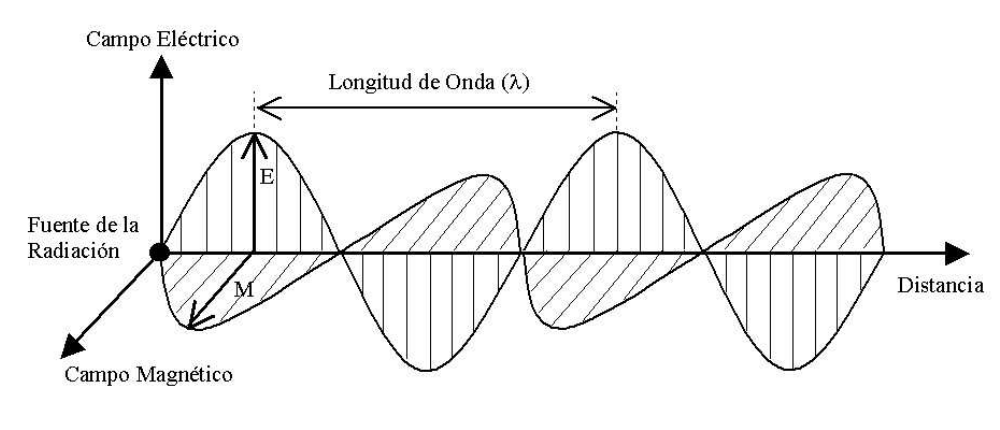
\includegraphics[width=.8\textwidth]{./images/propagacion.png}}
  \centering
  \caption{Se muestran los vectores eléctricos ($E$) y magnéticos ($M$), perpendiculares entre ellos,de una onda electromagnética. La longitud de onda ($\lambda$) corresponde a la distancia entre dos crestas consecutivas. \cite{chile}}
  \label{fPropagacion}
\end{figure}

Cuando se logra ver algo, no es directamente el objeto que se ve, sino la radiación electromagnética dentro del rango visual que emite dicho objeto y parte de la energía es absorbida por el objeto, ya que actúan con base en los componentes químicos que lo forman. El espectro electromagnético se divide en rangos(vea tabla \ref{tEspectro}).

También se le dice espectro electromagnético a la radiación electromagnética que absorbe o emite una sustancia. Dicha radiación sirve para identificar la sustancia de manera análoga a una huella dactilar lo cual será explicado en el siguiente subtema \ref{FirmasEspectrales}. Los espectros se pueden observar mediante espectroscopios que, además de permitir ver el espectro, permiten realizar medidas sobre el mismo, como son la longitud de onda, la frecuencia y la intensidad de la radiación.\\
Una cámara digital \textit{RGB} tradicional capta el espectro visible que responde a longitudes de onda 390 nm a 750 nm(vea la tabla \ref{tEV}). El objetivo de las cámaras tradicionales es dar como resultado una imagen en el rango de visibilidad humana. Lo interesante es cuando se toma en cuenta otros valores fuera del rango visible. (véase la Figura \ref{fNasa})

\begin{table}[]
\centering
\begin{tabular}{l|l|l|l|}
\cline{2-4}
                         & Color    & \begin{tabular}[c]{@{}l@{}}Intervalo de longitud\\ de onda ($\lambda$)\end{tabular} & \begin{tabular}[c]{@{}l@{}}Intervalo de \\ frecuencia ($\nu$)\end{tabular} \\ \cline{2-4}
\cellcolor[HTML]{FE0000} & Rojo     & $\sim$ 700 - 635 nm                                                               & $\sim$ 430 - 480 THz                                                 \\ \cline{2-4}
\cellcolor[HTML]{FFA500} & Naranja  & $\sim$ 635 – 590 nm                                                                & $\sim$ 480 – 510 THz                                                 \\ \cline{2-4}
\cellcolor[HTML]{FFFF00} & Amarillo & $\sim$ 590 – 560 nm                                                                & $\sim$ 510 – 540 THz                                                 \\ \cline{2-4}
\cellcolor[HTML]{008000} & Verde    & $\sim$ 560 – 520 nm                                                                & $\sim$ 540 – 580 THz                                                 \\ \cline{2-4}
\cellcolor[HTML]{00FFFF} & Cian     & $\sim$ 520 – 490 nm                                                                & $\sim$ 580 – 610 THz                                                 \\ \cline{2-4}
\cellcolor[HTML]{0000FF} & Azul     & $\sim$ 490 – 450 nm                                                                & $\sim$ 610 – 670 THz                                                 \\ \cline{2-4}
\cellcolor[HTML]{EE82EE} & Violeta  & $\sim$ 450 – 400 nm                                                                & $\sim$ 670 – 750 THz                                                 \\ \cline{2-4}
\end{tabular}
\caption{Espectro visible\cite{Craig}.}
\label{tEV}
\end{table}

\begin{table}[]
\centering
\begin{tabular}{|l|l|l|}
\hline
\multicolumn{1}{|c|}{\textbf{\begin{tabular}[c]{@{}c@{}}Región o Banda\\ Espectral\end{tabular}}} & \multicolumn{1}{c|}{\textbf{\begin{tabular}[c]{@{}c@{}}Longitud \\ de onda $\lambda$\end{tabular}}}         & \textbf{Características}                                                                                                                                                                                           \\ \hline
Rayos Gamma                                                                                       & \textless 0.03 nm                                                                                        & \multirow{2}{*}{\textit{\begin{tabular}[c]{@{}l@{}}Radiación completamente absorbida\\ por las capas superiores de la \\ atmósfera. No se utilizan en \\ teledetección.\end{tabular}}}                                                                                  \\ \cline{1-2}
\\Rayos X  \\                                                                                         & 0.03 - 30 nm                                                                                             &                                                                                                                                                                                                                                                                          \\ \hline
Ultravioleta (UV)                                                                                 & 0.03 - 0.4 $\mu$m                                                                                            & \textit{\begin{tabular}[c]{@{}l@{}}La radiación con $\lambda$ \textless 0.3 $\mu$m es\\ completamente absorbida por la capa\\ de ozono de la atmósfera.\end{tabular}}                                                                                                           \\ \hline
\begin{tabular}[c]{@{}l@{}}Visible (azul,verde\\ y rojo)\end{tabular}                             & \begin{tabular}[c]{@{}l@{}}0.4 - 0.5 $\mu$m (azul)\\ 0.5 - 0.6 $\mu$m (verde)\\ 0.6 - 0.7 $\mu$m (rojo)\end{tabular} & \textit{\begin{tabular}[c]{@{}l@{}}Se puede detectar a través de \\ fotodetectores y películas fotosensibles\\ normales (color B/N).\end{tabular}}                                                                                                                       \\ \hline
Infrarrojo reflejado                                                                              & \begin{tabular}[c]{@{}l@{}}0.7 - 1.3 $\mu$m \\ (IR cercano)\\ 1.3 - 3.0 $\mu$m \\ (IR medio)\end{tabular}        & \textit{\begin{tabular}[c]{@{}l@{}}Radiación solar reflejada que no\\ contiene información acerca de las\\ propiedades térmicas de los materiales.\\ El rango 0.7 a 0.9 $\mu$m se puede \\ detectar usando películas fotosensibles\\ (infrarrojo fotográfico).\end{tabular}} \\ \hline
Infrarrojo térmico                                                                                & \begin{tabular}[c]{@{}l@{}}3.0 - 5.0 um\\ 8.0 - 14.0 um\end{tabular}                                     & \textit{\begin{tabular}[c]{@{}l@{}}Corresponden a dos ventanas\\ atmosféricas en la región térmica.\end{tabular}}                                                                                                                                                        \\ \hline
\begin{tabular}[c]{@{}l@{}}Radar (región de \\ las microondas)\end{tabular}                       & 0.1 - 100 cm                                                                                             & \textit{\begin{tabular}[c]{@{}l@{}}Radiación de grandes longitudes de\\ onda, capaces de penetrar nubes,\\ nieblas y lluvia.\end{tabular}}                                                                                                                               \\ \hline
Ondas de Radio y TV                                                                               & \textgreater 100 cm                                                                                      & \textit{\begin{tabular}[c]{@{}l@{}}Radiación con las mayores longitudes\\ de onda del espectro. Se utilizan en \\ telecomunicaciones.\end{tabular}}                                                                                                                      \\ \hline
\end{tabular}
\caption{Descripción de las regiones del espectro electromagnético ($1 \mu m = 10^{-6}$ m y 1 nm = $10^{-9} m$)\cite{chile}.}
\label{tEspectro}
\end{table}


%Craig F. Bohren (2006). Fundamentals of Atmospheric Radiation: An Introduction with 400 Problems. Wiley-VCH. ISBN 3-527-40503-8.

\begin{figure}[h]
  \centering
  \framebox[14cm]{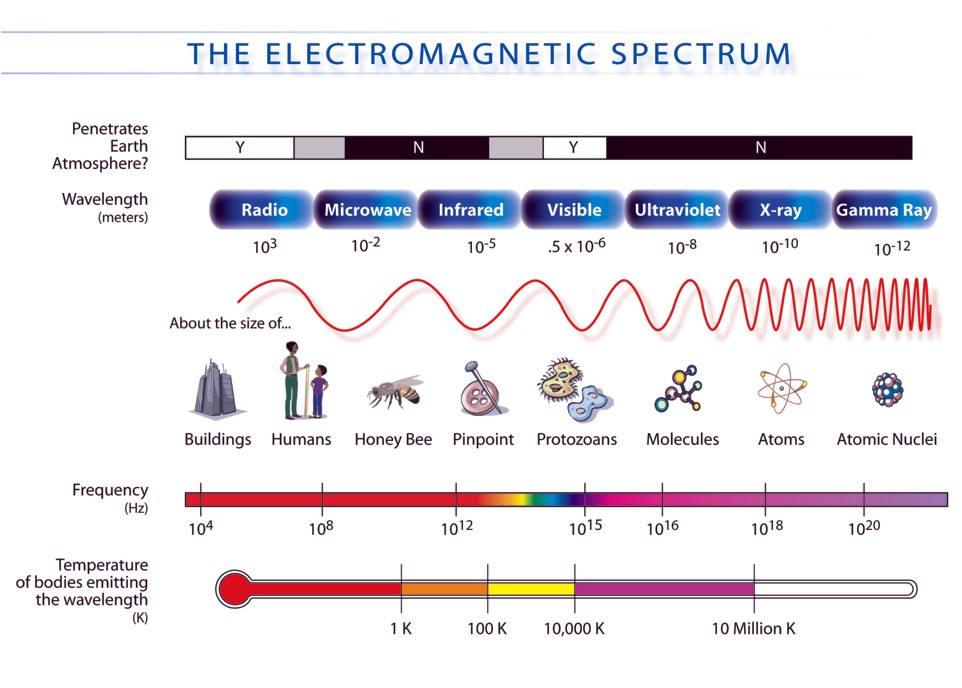
\includegraphics[width=.8\textwidth]{./images/nasa.jpg}}
  \centering
  \caption{Diagrama del espectro electromagnético \cite{nasaimage}.}
  \label{fNasa}
\end{figure}
\subsection{Firmas espectrales}
\label{FirmasEspectrales}
La firma espectral es la variación de reflectancia de la radiación proveniente de la energía solar cuando tiene contacto con la superficie terrestre reflejada, absorbida y transmitida. La energía es reflejada cuando es rebotada, es absorbida cuando conserva energía provocando calor en el material y es transmitida cuando pasa a través del material. Como se comentó en el capítulo anterior, el espectro electromagnético es dado por la radiación emitida y absorvida por el objeto. Gracias a que cada elemento capturado emite radiación electromagnética recibida del sol de forma diferenciada, es posible mediante un análisis de los datos determinar qué elementos químicos lo forman y determinar qué es lo que se capto, tal como se puede ver en la Figura \ref{fFirma}. \cite{AVIRIS}

\begin{figure}[h]
  \centering
  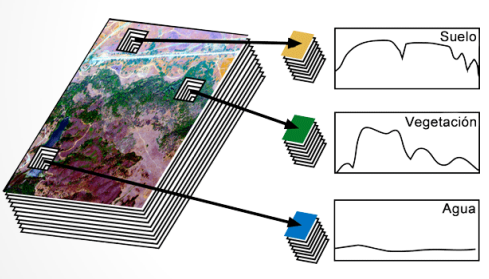
\includegraphics[width=.7\textwidth]{./images/firma.png}
  \centering
  \caption{Firmas espectrales de suelo, vegetación y agua. \cite{Quinones}.}
  \label{fFirma}
\end{figure}
%IMÁGENES HIPERESPECTRALES: ANÁLISIS Y APLICACIONES. Sebastián Quiñones F. Cartógrafo Centro de Ecología Aplicada
Otra de las aplicaciones muy comunes es detectar la sanidad de las plantas tomando en cuenta las variables ya mencionadas como se puede observar en un ejemplo en la Figura \ref{fSanidad}. También se han utilizado estas técnicas en detección de sanidad en animales \cite{animal} como se ve en la Figura \ref{fAnimal}. \cite{medical}

\begin{figure}[h]
  \centering
  \framebox[14cm]{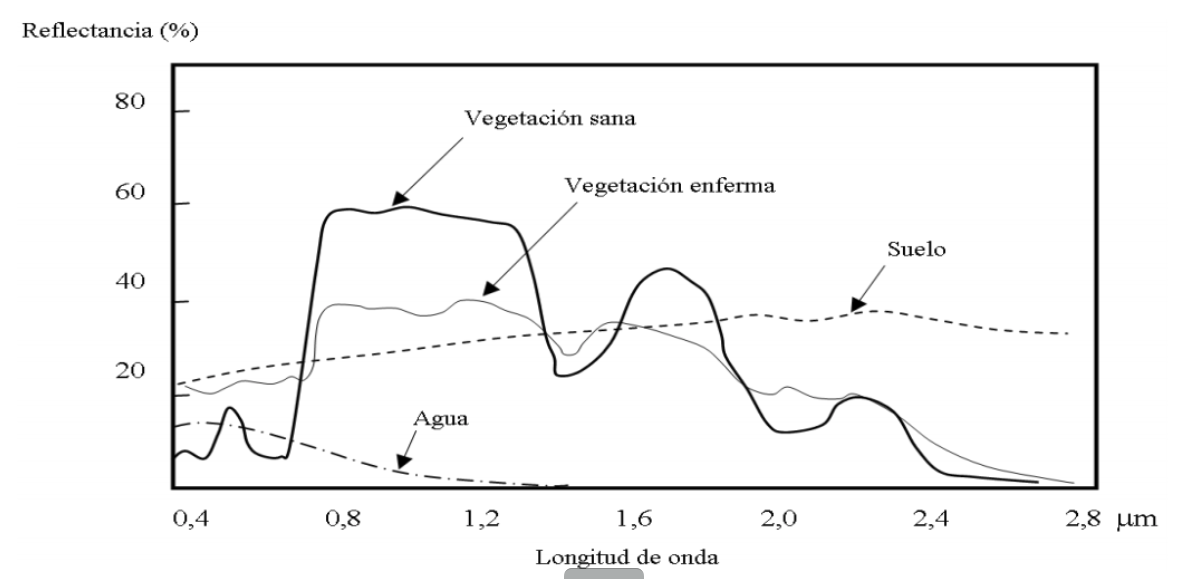
\includegraphics[width=.8\textwidth]{./images/sanidad.png}}
  \centering
  \caption{Detección de sanidad en vegetales \cite{chile}.}
  \label{fSanidad}
\end{figure}

\begin{figure}[h]
  \centering
  \framebox[5cm]{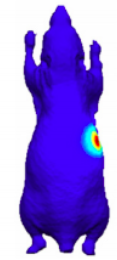
\includegraphics[width=.2\textwidth]{./images/animal.png}}
  \centering
  \caption{Detección espectral de anormalidades en animales. \cite{animal}.}
  \label{fAnimal}
\end{figure}
%Abhijit J Chaudhari and Felix Darvas and James R Bading and Rex A Moats and Peter S Conti and Desmond J Smith and Simon R Cherry and Richard M Leahy, “Hyperspectral and multispectral bioluminescence optical tomography for small animal imaging,” in Physics in Medicine and Biology, vol. 50, 2005
\subsection{Imagen espectral}
Tomando en cuenta que una imagen es la reproducción de una figura por la combinación de los rayos de luz y que el espectro es la radiación electromagnética que es absorbida o emitida, se puede concluir que una imagen espectral es la reproducción de una figura de un objeto por la combinación de radiación emitida en cierta longitud de onda electromagnética (véase la Figura \ref{fWiki}).

\begin{figure}[h]
  \centering
  \framebox[14cm]{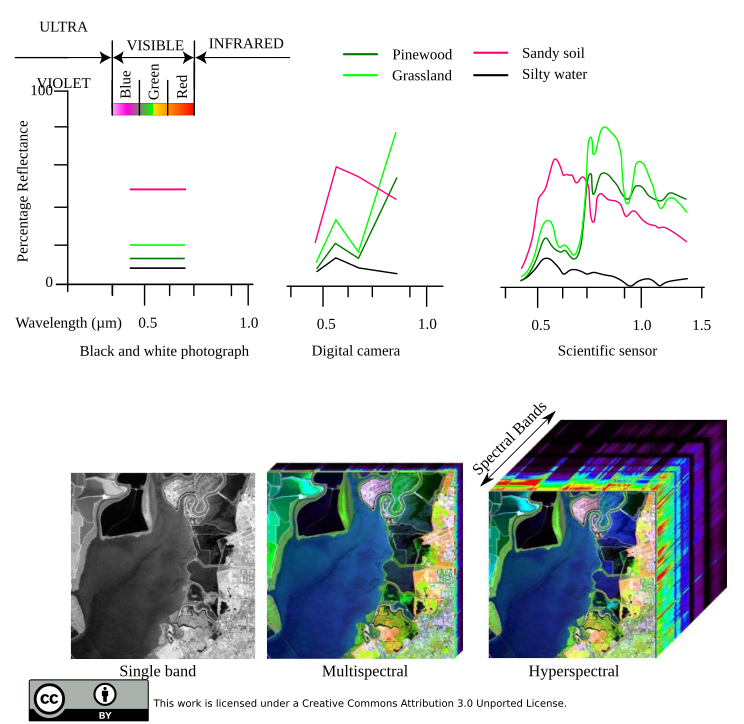
\includegraphics[width=.8\textwidth]{./images/wiki.png}}
  \centering
  \caption{Imagen hiperespectral, multiespectral y espectral.}
  \label{fWiki}
\end{figure}

\subsection{Imagen Multiespectral}
Las imágenes Multiespectrales son un conjunto de entre 3 a 20 imágenes de las mismas dimensiones (véase Figura \ref{fWiki}), reproduciendo una figura con base en diferentes rangos de longitud de onda electromagnética (véase la Figura \ref{fJairo}). Donde no necesariamente tienen que ser contiguas en los rangos tomados. Esto produce un arreglo de imágenes correspondientes a un mismo objeto o toma pero en diferentes longitudes de onda.

\begin{figure}[h]
  \centering
  \framebox[14cm]{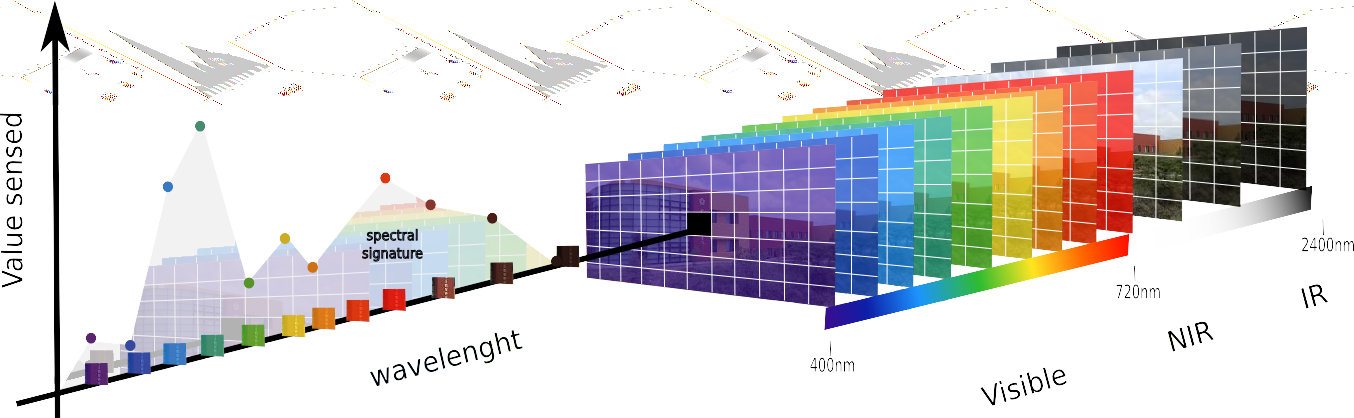
\includegraphics[width=.8\textwidth]{./images/jairo.png}}
  \centering
  \caption{Longitudes de onda \cite{FuzzyVD}.}
  \label{fJairo}
\end{figure}

\subsection{Imagen Hiperespectral}
El concepto de hiperespectral deriva de la toma de una gran cantidad de espectros de una superficie. Donde cada toma es obtenida para formar un cubo de la imagen.(véase la Figura \ref{fWiki})

Tomando en cuenta la información recolectada a lo largo del espectro electromagnético se forma un cubo de datos con el que se puede trabajar ya según la aplicación que se le quiera dar. Usando los principios de CTIS, la forma en que se captura una imagen hiperespectral es obteniendo el contenido espectral de cada pixel en una imagen 2D superposicionada. Esta tecnología divide los datos de la imagen pixel por pixel en bandas estrechas de longitud de onda, dando como resultado un cubo 3D de datos como se muestra en la Figura \ref{fPaper1}.\\

\begin{figure}[h]
  \centering
  \framebox[9cm]{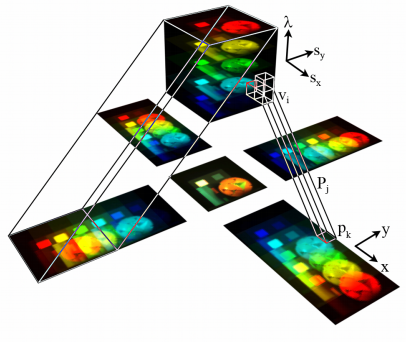
\includegraphics[width=.6\textwidth]{./images/paper1.png}}
  \centering
  \caption{Proyecciones paralelas de difracción \cite{PracCam}.}
  \label{fPaper1}
\end{figure}

\section{CTIS}
\label{CTIS}
El espectrómetro de imágenes por tomografía computarizada es utilizado para la captura de las imágenes hiperespectrales sin necesidad de escaneo puesto que es obtenido en un \textit{snapshot} que consiste en un único tiempo de integración gracias a un conjunto de detectores.
Funciona como si se tratara de dos cámaras en sí, donde una toma la imagen base en un cuadro de visión y la segunda capta la energía a distintas longitudes de onda electromagnética reflectada en el marco tomado.
Dando como resultado una imagen de referencia(zero mode) y los espectros captados a diferentes longitudes de onda basadas en dicha imagen.

Da como resultado una imagen 2D que es una superposición de los espectros, siendo el cubo hiperespectral proyectado de forma paralela en distintos ángulos (vea la Figura \ref{fPaper1}). El cubo formado es compuesto por voxeles ($V_i$), que son una unidad cúbica componente de la imagen hiperespectral definidos por la resolución de la imagen superposicionada.

La estructura del dispositivo CTIS son las presentadas en la Figura \ref{fCTIS}, donde la lente de imagen (\textit{imaging lens}) refleja la imagen a través de la apertura ya sea una imagen o conjunto de imágenes (\textit{slit/square aperture}). La luz divergente es hecha paralela al pasar por la \textit{lente de colimación} (\textit{collimation lens}), para después pasar por la rejilla de difracción (\textit{diffraction grating}). La luz difractada y no difractada se vuelven a hacer imágenes mediante el lente de reimagen (\textit{re-imaging lens}). Finalmente el resultante es captado por el sensor.

\begin{figure}[h]
  \centering
  \framebox[13cm]{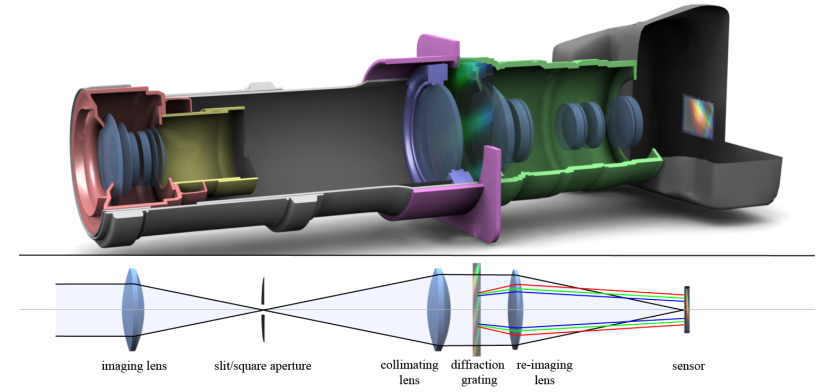
\includegraphics[width=.9\textwidth]{./images/CTIS.png}}
  \centering
  \caption{Estructura CTIS. \cite{PracCam}}
  \label{fCTIS}
\end{figure}

%Chapter 3 overview explain RGGB
\subsection{Calibración espacial}
%The spatial calibration localizes the positions of individual wavelenghts on the image grid (in slit mode), or determinesthe coefficients of the projection of the data cube.
%The calibration will allow a precise mapping from the projected image to wavelenghts in the spectrum.

La calibración espacial corrige distorsiones que tenga la imagen obtenida por el dispositivo CTIS. Lo que hace es buscar desalineamientos cuando pasa la luz entre la apertura y la rejilla de difracción.

\subsection{Calibración espectral}
%Calculates the spectral intensity response od the optical system and the sensor pixels. The pixels are arranged in a RGGB Bayer filter array, so each pixel responds more in the red, green or blue range of the spectrum. This means that similar to standard imaging, we need to apply demosaicing algorithms to recover the full spectra

El objetivo de la calibración espectral es ajustar la sensibilidad espectral de cada canal de color que se determinan identificando un espectro cuando es continuo y conocido con alta precisión.

\subsection{Medición de slit espectral e interpolación cromática}
Para la reconstrucción del verdadero espectro de la medición aplicando la calibración espectral $f(x,y)$ debemos tomar en cuenta las diferentes sensibilidades de los diferentes canales de color en el \textit{filtro Bayer} (\textit{Bayer filter} \cite{Bayer}).
Cualquier canal puede ser utilizado para reconstruir un espectro considerando que se tiene una respuesta por cada canal de color.
Puesto que la respuesta espectral de cada canal cubre sólo parte del espectro visible y las posiciones de los píxeles de Bayer están entrelazadas, se combinan las mediciones de píxeles de Bayer adyacentes con valores interpolados.
Para suprimir ruido los canales con peso (\textit{weight}) $W_{r,g,b}(\lambda)$ donde $r,g,b$ corresponden a los colores rojo(\textit{red}), verde(\textit{green}) y azul(\textit{blue}) basados en la amplitud de su respuesta espectral:
\begin{flalign}
  \label{FormulaMSS1}
  W_{r,g,b}(\lambda)=\frac{S_{r,g,b}(\lambda)}{\sum\limits_{c=r,g,b}S_{c}(\lambda)}.
\end{flalign}
después el espectro $M(\lambda)$ de una medida de respuesta $m_{r,g,b}(\lambda)$ es reconstruida con:
\begin{flalign}
  \label{FormulaMSS2}
  M(\lambda)=\sum\limits_{c=r,g,b}\frac{m_{c}(\lambda)}{S_{c}(\lambda)}w_{c}(\lambda)=\frac{\sum\limits_{c=r,g,b}m_{c}(\lambda)}{\sum\limits_{c=r,g,b}S_{c}(\lambda)}w_{c}(\lambda).
\end{flalign}
con valores interpolados donde fueron necesarios.


\subsection{Calibración hiperespectral}
La calibración hiperespectral consiste en usar la apertura cuadrada, puesto que tomando la apertura \textit{slit} solo se podrá tener una imagen a una cierta longitud de onda. En cambio utilizando la apertura cuadrada se podrá tomar un conjunto de imágenes a lo largo del espectro electromagnético, logrando así el cubo de datos.
\subsubsection{Teoría de reconstrucción CTIS} \cite{extra6} \cite{extra7}
Para la reconstrucción se toma en cuenta una matriz $H$ generada por la proyección paralela (vea capítulo \ref{CTIS}) que trabaja con el vector $\vec{f}$ que contiene voxeles del cubo de datos como se mostró en la Figura \ref{fPaper1}. $H$ es una matriz $M$ x $N$ donde $M$ es el número de píxeles en la imagen y $N$ el número de voxeles en el cubo de datos. Multiplicando la matriz por el vector $\vec{f}$ se obtiene un nuevo vector $\vec{g}$:
\begin{flalign}
  \label{FormulaCH1}
  \vec{g}=H\vec{f}.
\end{flalign}
Cada columna contiene cinco entradas en las posiciones difractadas que son la superior, inferior, a la izquierda, a la derecha y en el centro (zero mode). Como resultante de lo mencionado la matriz $H$ es muy grande por lo que se invierte la ecuación \ref{FormulaCH1}. Con la matriz $H$ se genera una primera suposición a través de $\vec{\hat{f}}0=H^T\vec g$ y se realiza la etapa iterativa de maximización de expectativas:
\begin{flalign}
  \label{FormulaCH2}
  \hat{f}_{n}^{k+1}=\frac
            {
              \hat{f}_{n}^{k}
            }
            {
              \sum\limits_{m=1}^{M}H_{mn}
            }
            \sum\limits_{m=1}^{M}
              H_{nm}^{T}
            \frac
            {
              g_{m}
            }
            {
              (H\hat{f}^{k})_{m}
            }.
\end{flalign}

\subsubsection{Calibración espacial hiperespectral}
Para calibrar la imagen hiperespectral se deberán tener identificadas las proyecciones correspondientes a cada espectro en las cinco entradas. Con base en la Figura \ref{fPaper1} se identifica la correspondencia de las proyecciones con base en las coordenadas $(x,y)$ de la imagen plana.
Si se deja a $P_{j}$ como proyecciones del cubo de datos $P_{j}(s_{x},s_{y},\lambda) = (x,y)$ construido por los voxeles $v_{i}=(s_{x_{i}},s_{y_{i}},\lambda_{i})$ que da cinco píxeles $p_k=(x_k,y_k)$ con índices $k \in 1...M$. Entonces $H$ puede ser construido mediante las cinco entradas $p_{k_1},...,p_{k_5}$ en la i-ésima columna de $H$ a uno.

Para que esto suceda se necesita determinar la posición de las cinco proyecciones para identificar alguna inclinación que tenga la imagen y poderlo revertir. Se toma una captura siendo $P_{0}$ el modo zero y $P_{1..4}(s_x,s_y,\lambda) = (x,y)$ (vea Figura \ref{fPaper1}), se alinean las $P_{1..4}$ en forma de cruz tomando como referencia central a $P_{0}$ mediante una interpolación lineal.

\subsubsection{Medición de imágenes hiperespectrales}
Al tener una imagen hiperespectral CTIS se necesita hacer una medición de las señales a distintas longitudes de onda para de esta forma identificar las caractarísticas superposicionadas de las diversas longitudes de ondas del espectro electromagnético.

Teniendo la matriz $H$ definida se puede proseguir para la solución de una imagen CTIS. Considerando que la utilización de la ecuación \ref{FormulaCH2} da una gran cantidad de ceros se tienen datos y procedimientos innecesarios. Para solucionar esto se propone separar por canal el arreglo de \textit{Mosaico de Bayer} tratando a los dos canales de verde (\textit{green} G) del \textit{arreglo Bayer RGGB}. Se realiza lo mismo con la matriz $H$ para extraer $H$ matrices para cada uno de los cuatro canales \textit{RGGB} solo para las longitudes de onda donde la correspondencia no sea cero.

\subsubsection{Interpolación cromática espacial y reconstrucción}
\label{Reconstruction}
La \textit{interpolación cromática} (\textit{demosaicing}) es el proceso que se realiza a un conjunto de muestras cromáticas tomadas de un sensor de imagen para producir una imagen a color.
Una vez realizada la interpolación cromática se podrá hacer la reconstrucción en la imagen CTIS.
Para lograr la reconstrucción se realiza una interpolación cromática, similar a la \textit{interpolación cromática} con imágenes RGB.
Posterior a ello se hace una interpolación bilineal para obtener los píxeles Bayer.
Una interpolación cromática espectral es diferente a las convencionales, por su información en superposición contenida.
Con el cubo de datos interpolados cromáticamente se recuperan los píxeles espectrales utilizando la ecuación \ref{FormulaMSS1}.
Mediante la configuración \textit{slit} se recolectan los valores por espectro, provocando de esta forma una integral para calcular la información en $S_{r,g,b}^l(\lambda_i)$ en resoluciones bajas:
\begin{flalign}
  \label{FormulaSDR}
  S_{r,g,b}^l(\lambda_i)=\int _{\lambda_i-\frac{r}{2}}^{\lambda_i+\frac{r}{2}}S_{r,g,b}(\lambda)d\lambda.
\end{flalign}

\cite{extra2}


\section{Mosaico de Bayer\cite{Bayer}}
El mosaico de Bayer es la interpolación en la imagen de dos muestras verdes, una roja y otra azul. Se tomó en cuenta el patrón Bayer \textit{RGGB} dejando en porcentaje 50\% de filtros verdes, un 25\% de rojos y un 25\% de azules en la imagen. La razón por la que se utilizan más muestras verdes es porque el ojo humano es más sensible a ese color.

Siendo el verde que aparece en todas las filas, los colores azul y rojo aparecen por fila uno y después el otro, denominando la fila roja cuando tiene rojo y verde, y fila azul cuando tiene azul y verde. Los verdes pueden aparecen en la posición par o la impar, alterado por el color de fila que se encuentre.
La fila con rojo tendría el patrón rojo, verde,rojo,verde,..., y el la fila con azul el patrón verde, azul, verde, azul,...

El patrón está desplegado en la Figura \ref{fBayer}.

\begin{figure}[h]
  \centering
  \framebox[9cm]{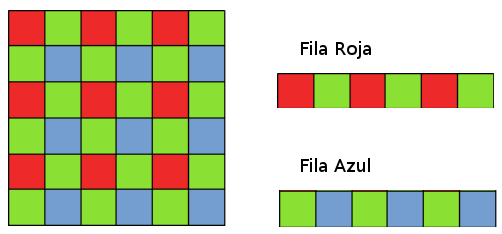
\includegraphics[width=.6\textwidth]{./images/Bayer.png}}
  \centering
  \caption{Patrón de Bayer.}
  \label{fBayer}
\end{figure}
%\subsection{Pseudocódigo}

%aplicado a imágenes wavelets0.
\section{Método de Malvar, He y Cutler}\label{capMalvar}
El método propuesto por Malvar, He y Culter deriva de una modificación de la interpolación bilineal e intenta atacar los problemas de la interpolación cromática. El algoritmo propuesto consta de un simple método lineal usando filtros 5x5. Para la interpolación cromática se utilizará la imagen pasada por una matriz de filtros de color (en inglés \textit{Color Filter Array} CFA) Bayer pattern\cite{Bayer}.

En localización del azul o rojo pixel, la interpolación bilineal del componente verde es el promedio de sus cuatro vecinos axiales,
\begin{flalign}
  \label{Malvar1}
  \hat{G}^{bl}(i,j)=
  \frac{1}{4}(
  G(i-1,j)+
  G(i+1,j)+
  G(i,j-1)+
  G(i,j+1)
  ).
\end{flalign}
La interpolación bilineal de los componentes azul y rojo son similares, la diferencia es que toman a sus cuatro vecinos diagonales.

La localización del componente verde en el pixel rojo está estimado como
\begin{flalign}
  \label{Malvar2}
  \hat{G}(i,j)=\hat{G}^{bl}(i,j)+\alpha \Delta _R(i,j),
\end{flalign}
donde $\Delta _R$ es el \textit{Laplaciano} discreto de cinco puntos del canal rojo,
\begin{flalign}
  \label{Malvar3}
  \Delta _R(i,j):=R(i,j)-\frac{1}{4}(R(i-2,j)+R(i+2,j)+R(i,j-2)+R(i,j+2)).
\end{flalign}
Para estimar el componente rojo en la localización del pixel verde,
\begin{flalign}
  \label{Malvar4}
  \hat{R}(i,j)=\hat{R}^{bl}(i,j)+\beta \Delta _G(i,j),
\end{flalign}
donde $\Delta _G$ es el Laplaciano discreto de nueve puntos del canal verde.
Para estimar un componente rojo en una localización de un pixel azul,
\begin{flalign}
  \label{Malvar5}
  \hat{R}(i,j)=\hat{R}^{bl}(i,j)+\gamma \Delta _B(i,j),
\end{flalign}
donde $\Delta _B$ es el discreto Laplaciano de cinco puntos del canal azul.

Los parámetros de $\alpha$, $\beta$ y $\gamma$ controlan el peso de los términos de conección Laplacianos,
\begin{flalign}
  \label{Malvar6}
  \alpha =\frac{1}{2},\text{  }\beta =\frac{5}{8},\text{  }\gamma \frac{3}{4}.
\end{flalign}


\section{Gaussian blur\cite{Blur}}\label{CapBlur}
El desenfoque Gaussiano (Gaussian blur) es un método que utiliza algorítmos matemáticos. Se basa en la función Gaussiana,
\begin{flalign}
  \label{Gauss1}
  f(x)=ae-\frac{{(x-b)}^2}{2c^{2}}
\end{flalign}
que aplicado a las imágenes mezcla poco los colores de los vecinos de los píxeles entre sí. Lo cual ocasiona que se pierdan detalles y se vea incluso borroso.
Para la aplicación de esta función en las imágenes utilizadas en el proyecto se utilizó matlab.

\section{Sharpender\cite{Sharp}}\label{capSharpender}
La nitidez(sharpender) es el proceso inverso a desenfoque, puesto que intenta dar forma a bordes y a detalles de la imagen.
Pretende dar más calidad en la imagen resaltando pequeños contrastes en los píxeles con respecto a sus vecinos.
Para la aplicación de esta función en las imágenes utilizadas en el proyecto se utilizó matlab.
\section{GPA}
El algorítmo Análisis General Anterior(en inglés \textit{General Analysis Prior} GAP) para la reducción de ruido impulsivo para imágenes hiperespectrales está basado en la minimización de la variación total.\cite{MatlabDenoising}
\subsection{Transformada de Fourier}
Las transformadas de Fourier han jugado un papel importante al referirse a algoritmos de reconstrucción y filtrado de imágenes. A continuación se dará un repaso a las series de Fourier que después serán referenciadas en uno de los algoritmos de filtrado de imágenes utilizado en el presente proyecto.
\subsubsection{Series de Fourier \cite{FourierBook}}
Una función periódica $g(x)$ con un periodo $T$ tal que
\begin{flalign}
	\label{Fourier1}
	g(x)=g(x+T), -\infty  < x < \infty
\end{flalign}
podrá ser representada como una serie de Fourier:
\begin{flalign}
	\label{Fourier2}
	g(x)=\sum \limits_{n=-\infty}^{\infty}G_{n}e^{\frac{i2\pi nx}{T}}.
\end{flalign}
La función $g(x)$ deberá ser integrable en un periodo y ser continua. La función $g(x)$ deberá tener extremos en un periodo.
El coeficiente $G_{n}$ puede ser determinado por la siguiente relación ortogonal:
\begin{flalign}
	\label{Fourier3}
	\int_{-\frac{T}{2}}^
	{\frac{T}{2}}
	dx\text{ }
	e^{\frac{i2\pi (m-n)x)}{T}}
	=
	\left [
	\frac
	{e^{\frac{i2\pi (m-n)x)}{T}}}
	{\frac{i2\pi (m-n))}{T}}
	\right ]_
	{-\frac{T}{2}}^
	{\frac{T}{2}}=
	T \frac{\sin \pi (m-n))}{\pi (m-n))}=
	T\delta _{m,n}
\end{flalign}
Los coeficientes $G_n$ pueden ser obtenidos como:
\begin{flalign}
	\label{Fourier4}
	G_n=\frac{1}{T}\int _{-\frac{T}{2}}^{\frac{T}{2}}dx\text{ }g(x)e^{\frac{-i2\pi nx}{T}}.
\end{flalign}
Si $g(x)$ tiene una discontinuidad en $x=x_0$, la expanción de la serie converge a:
\begin{flalign}
	\label{Fourier5}
	g(x_0)=\frac{g(x_{0-})+g(x_{0+})}{2}.
\end{flalign}
Todos los términos impares son utilizados, por lo que la expansión de la serie de Fourier queda así:
\begin{flalign}
	\label{Fourier6}
	g(x)=\frac{1}{2}+\frac{2}{\pi}sin(\frac{2\pi x}{T})+\frac{2}{3\pi}sin(\frac{6\pi x}{T})+...
\end{flalign}
Las tramas producidas por la serie converge a una onda cuadrada. En la Figura \ref{fFourier} se puede ver como al agregar más términos de la serie se produce la convergencia.

\begin{figure}[h]
  \centering
  \framebox[9cm]{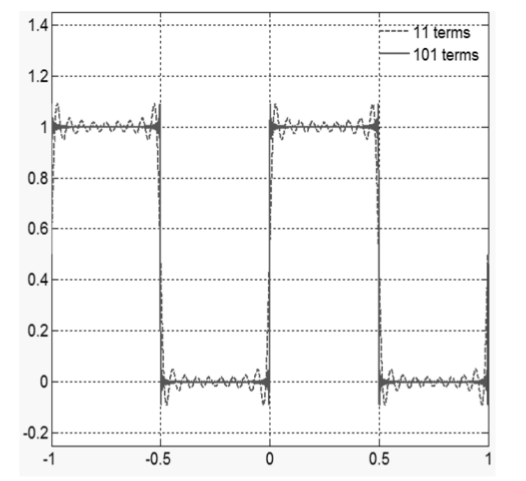
\includegraphics[width=.6\textwidth]{./images/fourier.png}}
  \centering
  \caption{Onda cuadrada representación de serie de Fourier con 11 y 101 terminos como en la ecuación \ref{Fourier6} \cite{FourierBook}.}
  \label{fFourier}
\end{figure}

%\subsubsection{Fenómeno de Gibbs}

\subsection{Transformadas de Wavalet} \cite{extra10}\cite{extra11}
Las wavelets son prácticamente mini ondas a diferencia de las infinitas como seno y coseno. La finalidad de que sean cortas es que puedan desvanecer rápidamente, limitadas en tiempo y frecuencia. A diferencia de la transformada de Fourier siendo infinita, la transformada de Wavalet es desarmada usando el mismo wavalet a diferentes escalas en vez de usar la misma frecuencia de seno vea Figura \ref{fWvsF}.

\begin{figure}[h]
  \centering
  \framebox[9cm]{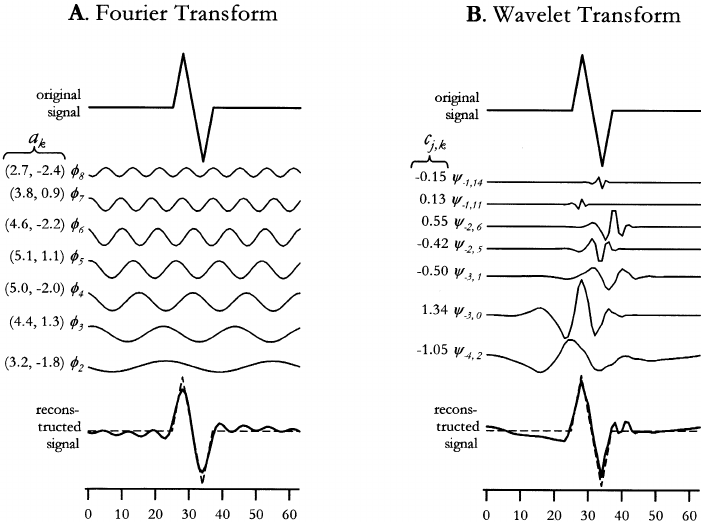
\includegraphics[width=.6\textwidth]{./images/waveletvsfft.png}}
  \centering
  \caption{Comparación entre transformada de Fourier y Wavelet \cite{WaveVsFourier}.}
  \label{fWvsF}
\end{figure}

Llamese $\varphi$ una base ortogonal del subespacio por escalación y transición se presenta la ecuación

\begin{flalign}
	\label{Dau1}
	\varphi _{i,j}(t)=\frac{1}{\sqrt{2}}\sum_{k\in \mathbf{Z}}h_k\varphi_{j+1,k}(t),
\end{flalign}

 siendo las funciones wavelets $\psi_{i,k}(t)$,  donde

 \begin{flalign}
	\label{Dau2}
	\psi_{i,k}(t)=\frac{1}{\sqrt{2}}\sum_{k\in \mathbf{Z}}g_k \varphi_{i+1,k}(t).
\end{flalign}

Se puede definir una transformada Wavelet como $f(t)$, donde

 \begin{flalign}
	\label{Dau3}
	f(t)=\sum_{j=0}^{J-1}\sum_{k=0}^{2^j-1}\omega _{j,k}\psi_{J,k}(t)+\sum_{k=0}^{L-1}s_{J,k}\varphi_{J,k}(t).
\end{flalign}

\subsubsection{Daubechies}\cite{Yakovlev} \label{rDau}%http://wwwmayr.in.tum.de/konferenzen/Jass05/courses/2/Yakovlev/Yakovlev_paper.pdf
Para obtener las transformadas Daubechies es necesario aplicar condiciones de momentos nulos(zero moments) a la función Wavelet que se le llamará función padre. Para hacer esto se deberán tener presentes las siguientes condiciones:

\begin{flalign}
  \label{Dau3}
  \left\{\begin{matrix}
  h_0+h_1+h_2+h_3=\sqrt{2}
  \\ h_1+2h_2+3h_3=0
  \\ h_0^2+h_1^2+h_2^2+h_3^2=1
  \\ h_0h_2+h_1h_3=0
\end{matrix}\right.
\end{flalign}
donde las soluciones serían:
\begin{flalign}
	\label{Dau3}
	h_0=\frac {1+\sqrt{3}}{4\sqrt{2}},\text{  }
	h_1=\frac{3+\sqrt{3}}{4\sqrt{2}},\text{  }
	h_2=\frac{3-\sqrt{3}}{4\sqrt{2}},\text{  }
	h_3=\frac{1-\sqrt{3}}{4\sqrt{2}}.
\end{flalign}

En la Figura \ref{fDau} se puede observar un ejemplo de \textit{wavelength} aplicando las condiciones de momentos nulos en contraste con una función general Wavelet.

\begin{figure}[h]
  \centering
  \framebox[9cm]{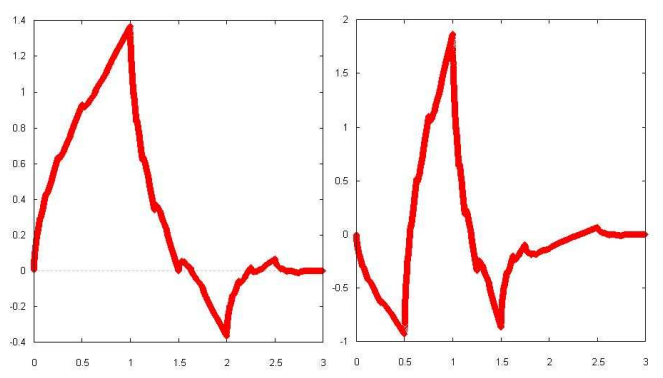
\includegraphics[width=.6\textwidth]{./images/dau.png}}
  \centering
  \caption{Daubachies y función wavelet \cite{Yakovlev}.}
  \label{fDau}
\end{figure}
%http://wwwmayr.in.tum.de/konferenzen/Jass05/courses/2/Yakovlev/Yakovlev_paper.pdf
%Theoretical framework
%\chapter{Propuesta} % Main chapter title
\label{Capitulo3} % Change X to a consecutive number; for referencing this chapter elsewhere, use \ref{ChapterX}
\lhead{\emph{Propuesta}}

%----------------------------------------------------------------------------------------
%	SECTION 1
%----------------------------------------------------------------------------------------
%algorithm uses Daubechies wavelet for spatial dimension and Fourier transform for vertical dimension. 
\section{Proceso}
Como se pudo capitalizar en el marco teórico del documento, los diversos pasos para llegar al resultado esperado constan de mejoras que se realizarían después de la etapa de obtención de los las imagenes hiperespectrales realizadas por la camara con estructura CTIS. Los métodos (o por decir de otra forma, filtros) son independientes entre sí, por lo que uno de ellos no necesita de la ejecución de otro previo para poderse aplicar. 
La propuesta se basa en utilizar uno, o combinación de los siguientes métodos encontrando así el mejor camino hacia el resultado esperado:

\begin{itemize}
\item Daubichies.
\item Slices.
\item Mosaic-Malvar.
\item Blur-Shparpender.
\end{itemize}

Donde cada uno de dichas combinaciones será probada por la calidad percibida mediante el ojo humano. 
Para poder analizar las imágenes se establecieron rutas de resultados que se muestran en la Figura \ref{pics:squeme}, donde se utilizaron diversas combinaciones de la teoría mostrada en los capítulos anteriores.
\clearpage
\begin{figure}[h]
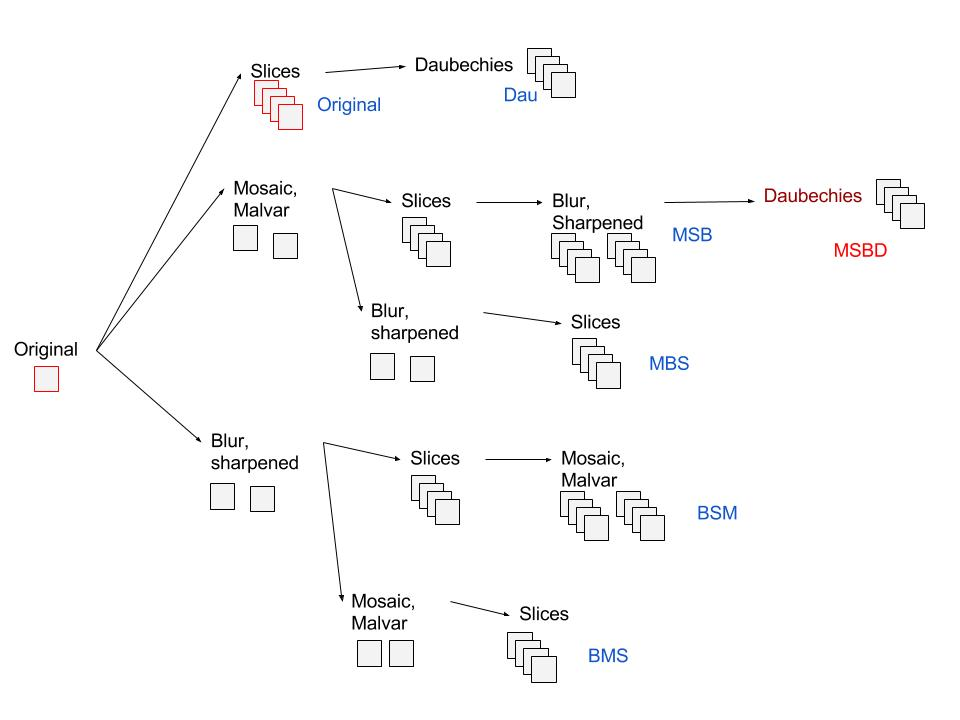
\includegraphics[scale=.4]{./images/RESULTS/squeme.jpg}
\caption{Esquema de resultados.}
\label{pics:squeme}
\end{figure}
Cada cuadro corresponde a una imagen superposicionadas y el conjunto de imágenes a las obtenidas por el procedimiento de abstracción por longitud de onda electromagnética de la imagen suporposicionada. %State of the art
%
\chapter{Resultados} % Main chapter title
\label{Capitulo4}
\lhead{\emph{Resultados}}

\section{Imágenes obtenidas}
La Figura \ref{pics:originalHDR} muestra la imagen HDR captada por la cámara hiperespectral de donde fueron sacadas las diversas imágenes por longitud de onda espectral mostradas en la Figura \ref{pics:slices}. La toma fue adquirida mediante la utilización de la cámara hiperespectral que fue utilizada mediante el uso de un software especializado, controlando dicho aparato. La toma fue una sola, que captó un marco de visión a diversas longitudes de onda.
\begin{figure}[h]
\begin{center}
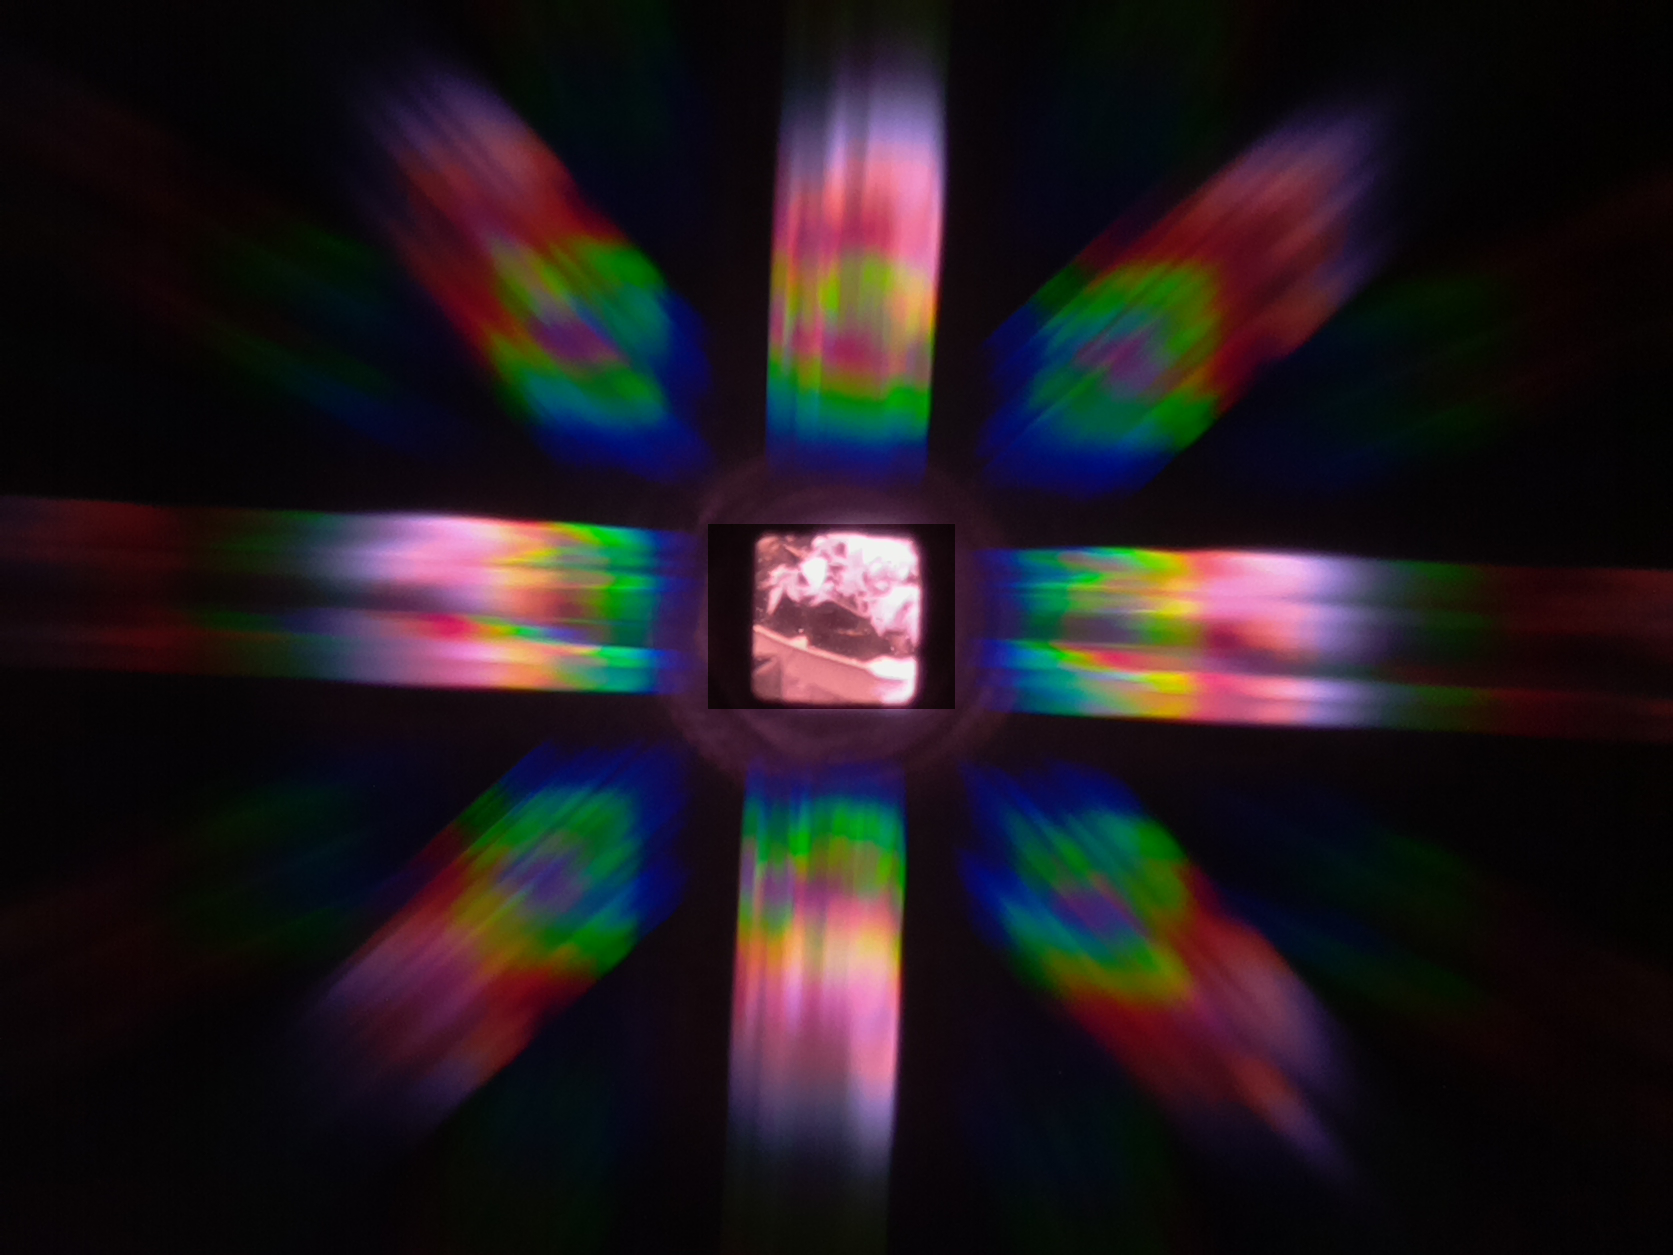
\includegraphics[scale=.3]{./images/RESULTS/original.png}
\end{center}
\caption{Imagen obtenida con camara hiperespectral.}
\label{pics:originalHDR}
\end{figure}

\begin{figure}[h]
\begin{center}$
\begin{array}{lll}
\subfloat[Imagen 466-637]{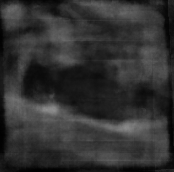
\includegraphics[scale=.99]{./images/RESULTS/slices/466.png}}&
\subfloat[Imagen 508-867]{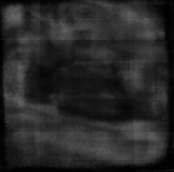
\includegraphics[scale=.99]{./images/RESULTS/slices/508.png}}&	
\subfloat[Imagen 549-087]{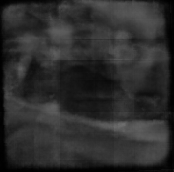
\includegraphics[scale=.99]{./images/RESULTS/slices/549.png}}
\end{array}$
\end{center}

\begin{center}$
\begin{array}{lll}
\subfloat[Imagen 589-307]{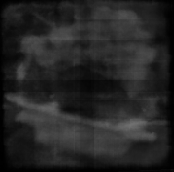
\includegraphics[scale=.99]{./images/RESULTS/slices/589.png}}&
\subfloat[Imagen 627-516]{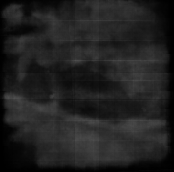
\includegraphics[scale=.99]{./images/RESULTS/slices/627.png}}&
\subfloat[Imagen 669-746]{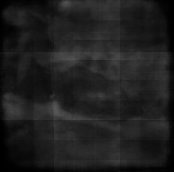
\includegraphics[scale=.99]{./images/RESULTS/slices/669.png}}
\end{array}$
\end{center}

\begin{center}$
\begin{array}{lll}
\subfloat[Imagen 709-966]{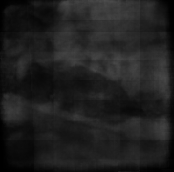
\includegraphics[scale=.99]{./images/RESULTS/slices/709.png}}&
\subfloat[Imagen 750-186]{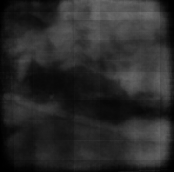
\includegraphics[scale=.99]{./images/RESULTS/slices/750.png}}&
\subfloat[Imagen 790-406]{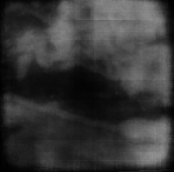
\includegraphics[scale=.99]{./images/RESULTS/slices/790.png}}
\end{array}$
\end{center}

\begin{center}$
\begin{array}{lll}
\subfloat[Imagen 830-625]{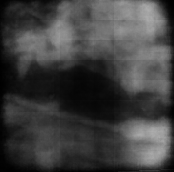
\includegraphics[scale=.99]{./images/RESULTS/slices/830.png}}&
\subfloat[Imagen 870-845]{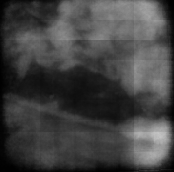
\includegraphics[scale=.99]{./images/RESULTS/slices/870.png}}&
\subfloat[Imagen 911-065]{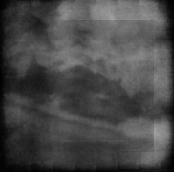
\includegraphics[scale=.99]{./images/RESULTS/slices/911.png}}
\end{array}$
\end{center}
\caption{Slices originales.}
\label{pics:slices}
\end{figure}

\clearpage
Con base en la Figura \ref{pics:squeme} los resultados tomados en consideración fueron el "Dau" que consta en aplicarle a los slices (conjunto de imágenes obtenidas mediante el método de obtención de imágenes por espectro CTIS) de la imagen hiperespectral el filtro utilizando la teoría de Daubichies (cápitulo \ref{rDau}), el MSB que consiste en la aplicación a la imagen original el Mosaic-Malvar y a ese resultado convertir la imagen HDR en slices para posterior aplicarle el Blur-Sharpened, además el MBS que de igual manera comienza aplicando el método de Moisac-Malvar seguido por el Blur-Sharpened y a ello después sacar los slices de la imagen hiperespectral, también el BSM que constaba en aplicarle a la imagen original el Blur-Sharpened seguido de sacar los slices y a ellos aplicarle el Mosaic-Malvar y por final se tomó el resultado BMS que era aplicarle a la imagen original el Bayer-Shapened y a ese resultado el Mosaic-Malvar para sacar los slices de la imagen superposicionada.

Para comparar los resultados se tomaron solo la imagen 870-845. Dichos resultados se muestran en la Figura \ref{pics:comparation}.

\begin{figure}[h]
\begin{center}$
\begin{array}{lll}
\subfloat[Original]{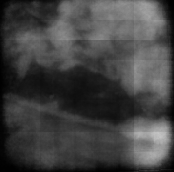
\includegraphics[scale=.99]{./images/RESULTS/compare870/original.png}}&
\subfloat[Dau]{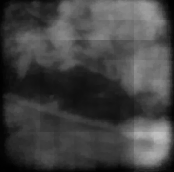
\includegraphics[scale=.7419]{./images/RESULTS/compare870/Dau.png}}&
\subfloat[MSB]{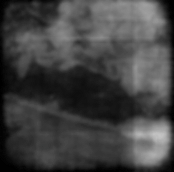
\includegraphics[scale=.7419]{./images/RESULTS/compare870/MSB.png}}
\end{array}$
\end{center}

\begin{center}$
\begin{array}{lll}
\subfloat[MBS]{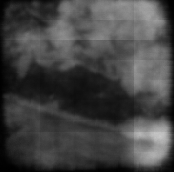
\includegraphics[scale=.99]{./images/RESULTS/compare870/MBS.png}}&
\subfloat[BSM]{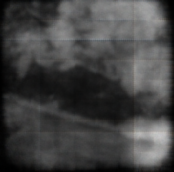
\includegraphics[scale=.7419]{./images/RESULTS/compare870/BSM.png}}&
\subfloat[BMS]{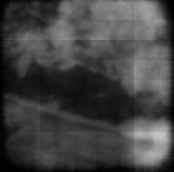
\includegraphics[scale=.99]{./images/RESULTS/compare870/BMS.png}}
\end{array}$
\end{center}

\caption{Comparación de resultados en imagen 870-845.}
\label{pics:comparation}
\end{figure}

Los resultados por los que se fueron obteniendo las imagenes se muestran en la Figura \ref{pics:process}, donde la imagen M es la imagen HDR original sometida a Malvar, MS es el resultado anterior sometido a el procedimiento de extracción de cubos. De ahí los slices se somente a Blur y sharpened resultando la imagen a comparar MSB. Y para finalizar el procedimiento se somete a la transformadas Daubichies para un último filtro dando como resultado la imagen MSBD.

\begin{figure}[h]
\begin{center}
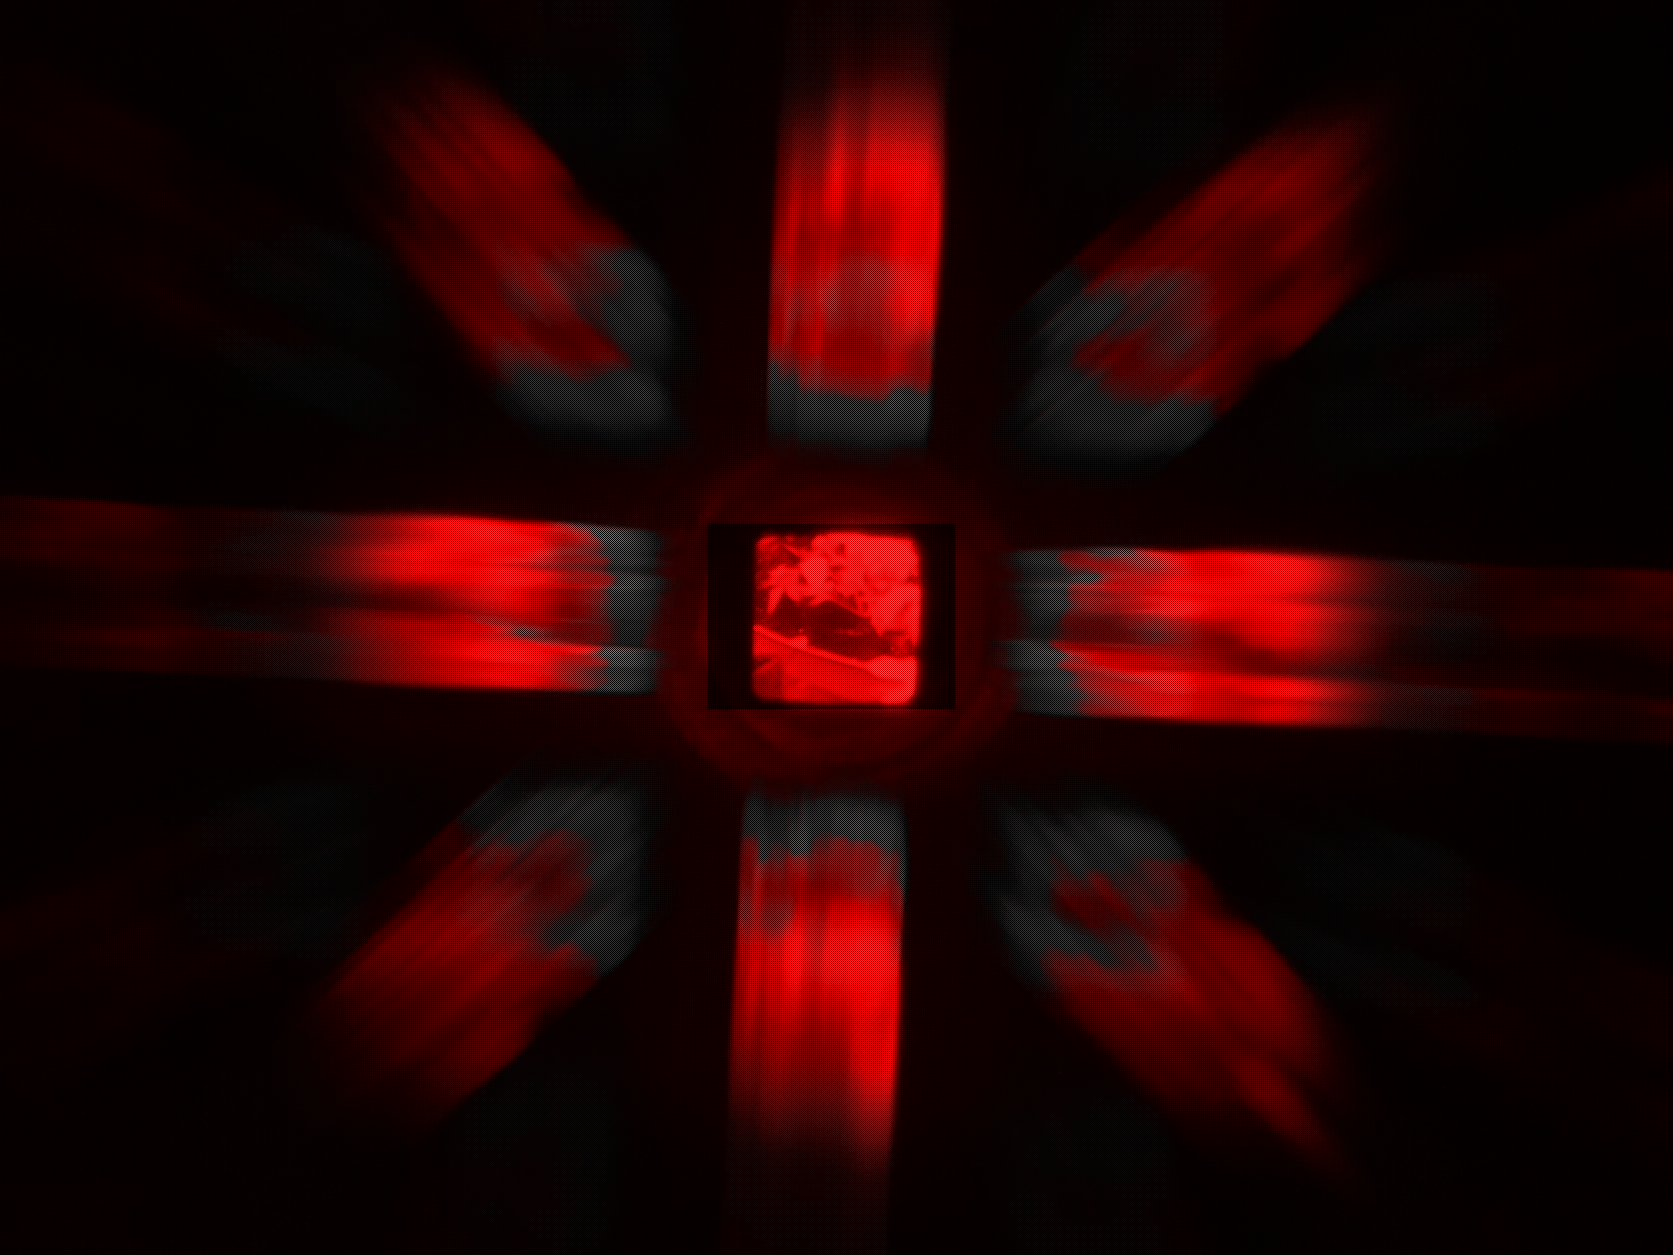
\includegraphics[scale=.2256]{./images/RESULTS/Malvar/mosaic.png}
\end{center}
\caption{Imagen obtenida con camara hiperespectral.}
\label{pics:originalHDR}
\end{figure}

\clearpage
\begin{figure}[h]
\begin{center}$
\begin{array}{lll}
\subfloat[MS]{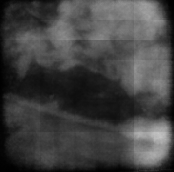
\includegraphics[scale=1.5]{./images/RESULTS/compare870/MS.png}}
\end{array}$
\end{center}

\begin{center}$
\begin{array}{lll}
\subfloat[MSB ]{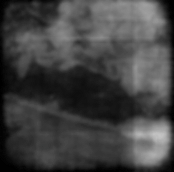
\includegraphics[scale=1.1]{./images/RESULTS/compare870/MSB.png}}&
\subfloat[MSBD]{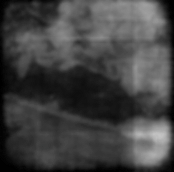
\includegraphics[scale=1.1]{./images/RESULTS/compare870/MSBD.png}}
\end{array}$
\end{center}

\caption{Proceso para MSBD en extracción 870-845.}
\label{pics:process}
\end{figure}
En las imágenes se muestran los resultados con base en los procedimientos explicados en el capítulo \ref{Capitulo2} y presentados en la Figura \ref{pics:squeme}.%Porpose (FuzzyVD and SMV_Perp)
%% Chapter Template
\chapter{Conclusiones} % Main chapter title
\label{Capitulo5} % Change X to a consecutive number; for referencing this chapter elsewhere, use \ref{ChapterX}
\lhead{\emph{Conclusiones}}

%----------------------------------------------------------------------------------------
%	SECTION 1
%----------------------------------------------------------------------------------------
Dentro de la descripción de la Hipotesis se menciona como objetivo lograr una mejora posterior al aplicar el procedimiento CTIS mediante filtrados diversos que puedieran eliminar ruido de las imágenes hiperespectrales resultantes. 

Mediante la utilización Mosaico Bayer y método de Malvar (vea \ref{capMalvar}) previo a la generación de imágenes de cubo hiperespectral, se pudo permitir que el resultado tuviera una mejora significante.
Después de obtener dicho resultado se aplica el método CTIS para obtener las imágenes y a estas imágenes se le aplica el desenfoque (vea capítulo \ref{CapBlur}) y la nitidez (véa \ref{capSharpender}) como último paso en el proceso.

Posterior a ello se aplicaron las series de Daubichies (vea la sección \ref{rDau}) que fueron descartados ya que no se presento algúna mejora notable al ser aplicado dejando el desenfoque y la nitidez como pasos definitivos.

La forma en que se comprobo la mejora fue visual, ya que por ser se tenían imagenes sin ruido con las cuales validar. Esto debido a que se trabajó directamente con imagenes abstraidas de la camara \ref{} con estructura CTIS.

Gracias a la aportación dada el presente proyecto se podrá dar una mejora con la cual será posible obtener un acercamiento a un producto con mayor madurez capaz de dar como resultado imagenes con mayor calidad(conservando detalles y eliminando ruido).


\begin{figure}[h]
\begin{center}$
\begin{array}{lll}
\subfloat[Original]{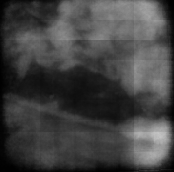
\includegraphics[scale=1.5]{./images/RESULTS/compare870/original.png}}&
\subfloat[MSB]{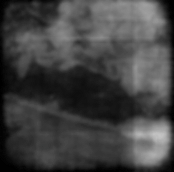
\includegraphics[scale=1.125]{./images/RESULTS/compare870/MSB.png}}
\end{array}$
\end{center}

\caption{Proceso para MSBD en extracción 870-845.}
\label{pics:process}
\end{figure}%Discusion( Experiments and results)
%\input{Chapters/Chapter6}%Conclusions

%----------------------------------------------------------------------------------------
%	CHAPTER: Introduction
%----------------------------------------------------------------------------------------

\chapter{Introduction} % Main chapter title

\label{ChapterIntroduction} % For referencing the chapter elsewhere, use \ref{Chapter1} 

\lhead{Chapter 1. \emph{Introduction}} % This is for the header on each page - perhaps a shortened title

This chapter provides an overview about the hyperspectral image analysis, their applications 
and previously works developed on this research field. Afterwards, it gives a description 
of the main problem studied in this thesis, and the motivation to propose new solutions for 
the problem.

%Furthermore, exposes the aims pursued and the original contributions reached. 

\section{Background}

A Hyperspectral Image (HI) is a set of two dimensional digital images acquired simultaneously 
from a physical surface where each image express the electromagnetic energy sensed at a specific 
wavelength. Typically, they are in the spectrum range of 0.4-2.5$\mu m$ with continuous and narrow 
separation of 0.004-0.01$\mu m$. Given that each image in the HI has the same area, each pixel 
represents exactly the same spatial area that the same pixel in the other images. \\

\begin{figure}[ht]
  \centering
  \framebox[14cm]{\includegraphics[width=13cm]{./ParaTesisDeMaestria/HypImg.png}}
  \centering
  \caption{A hyperspectral image. Redrawn from \cite{BioucasSurvey}.}
  \label{HIFigure}
\end{figure}


The application fields of hyperspectral image analysis has been increasing in the last 
years because the availability of new devices for hyperspectral image acquisition and 
public hyperspectral datasets (e.g. AVIRIS\cite{AVIRIS} or USGS\cite{USGS}). The high 
spectral resolution of these images, allows to develop different algorithms for target 
detection, material mapping, and material identification for applications in 
Agriculture \cite{Applications}, Security and Defense \cite{Applications}, Industry 
\cite{Applications}, etc.\\

In some applications, it is possible to perform target detection 
and material mapping, measuring in laboratory the light refraction, light emission, 
and light abortion at different wavelengths that each material of interest generates, 
identifying its specific pattern or \emph{spectral signature} (Definition 
\ref{DefSpectralSignature}). \\

However, for many other applications, there is not enough available prior 
information, or spectral signatures. For example, in many applications of remote sensing or 
precision agriculture, material distribution is required to obtain a correct 
classification of the pixels present in the HI. For this type of applications, it is necessary 
to decompose the scene in the respective \emph{abundances composition of the pure spectral 
signatures, or the constituent spectral, referred to as \textbf{endmembers}} \cite{Alina}. 
For this type of applications, it is possible to summarize the hyperspectral image analysis 
process as follows: estimate the total number of endmembers present in the HI, identify the 
endmember pixels, and unmix the original scene using the set of endmembers extracted in 
order to be able to target detection, target identification and material mapping. It is 
possible to estimate the number of endmembers present in the HI using the 
HFC \cite{HFC-NWHFC}, NWHFC \cite{HFC-NWHFC}, or TEP \cite{EIGENENERGY} algorithms. 
In order to identify the set of endmembers, 
the Endmember Extraction Algorithms (EEAs) use Statistical Methods (SM) \cite{Dimitris}, Orthogonal 
Subspace Projections (OSP) \cite{EIGENENERGY}, Linear Mixing Models (LMM) \cite{NFINDR}, etc., 
there are several EEAs (e.g. N-FINDR \cite{NFINDR}, SGA\cite{SGA}, PPI\cite{PPI}, OBA \cite{OBA}, 
ATGP \cite{ChangBig2013}, and others). One of the most used technique by the EEAs is the LMM 
because the convex nature of the hyperspectral dataset 
and the spatial resolution. This type of algorithms search the set of spectral pixels that inscribe 
the simplex \cite{PeterLax} of maximal volume, by assuming that all of them are endmembers and the 
remainder \emph{spectral pixels} (Definition \ref{DefHyperspectralPixel}) are linear combination of them \cite{NFINDR}. 
The (Figure \ref{FigureSinplexes}) 
provides fourth different simplexes. Finally, 
the unmixing processes can be performed using the methods proposed by \emph{Winter} \cite{NFINDR}, 
the procedure proposed by \emph{Tao et al.} \cite{OBA}, etc. \\

\begin{figure}[ht]
  \centering
  \framebox[14.5cm]{\includegraphics[width=12.5cm, height=4.25cm]{./ParaTesisDeMaestria/Simplexes.png}}
  \centering
  \caption{ (a-d) Simplex of maximal volume in $\mathbb{R}^0$, $\mathbb{R}^1$, $\mathbb{R}^2$, and $\mathbb{R}^3$ 
  respectively.}
  \label{FigureSinplexes}
\end{figure}

The present thesis explores the idea of building a deterministic method to estimate the simplex of 
maximal volume using a bottom-up approach by taking advantage of the LMM assumptions. As a result, 
the proposed algorithm SMV$\perp$ is based on the use of orthogonal complements \cite{PeterLax} 
and the Gram-Schmidt process \cite{Klaus}. In order to prove its efficiency, SVM$\perp$ has 
been compared against N-FINDR, ATGP and OBA because they are 
the algorithms that show the greatest similarity to SMV$\perp$ through the literature of endmember 
identification. The measurements used for comparison were the \emph{computational time complexity}, 
\emph{execution time}, and \emph{the final volume of the simplex in $\mathbb{R}^n$}. 
This is due to their accuracy to evaluate the performance of the algorithms for LMM. 
Furthermore, many EEAs including SMV$\perp$, require to estimate previously the number 
of endmembers to be extracted. In this thesis is proposed the FuzzyVD algorithm to estimate 
the number of endmembers present in a hyperspectral image. FuzzyVD facilitates the hyperspectral 
image analysis process because it does not require threshold setting, 
prior information, noise removal, dimensional reduction, low information band 
removal, water absorption band removal nor calculating the eigenvalues \cite{VD}. 
In order to do this, FuzzyVD 
exploits the properties of the SMV$\perp$ algorithm, 
fuzzy equivalence relations \cite{Klir}, fuzzy Minkowski distance\cite{Klir}, 
fuzzy logic \cite{Klir} and fuzzy systems \cite{Klir}, improving the reliability of 
the methods currently present in the literature, avoiding the threshold setting 
(estimate this, some times is as difficult as estimate the number of endmembers present in the HI), 
and expands the application field of fuzzy logic and fuzzy systems into the hyperspectral 
images analysis. 
FuzzyVD also provides a method to design fuzzy systems to define a total order in a set of 
possible partitions when desirable characteristics are well known. This algorithm has been 
applied to real AVIRIS \cite{AVIRIS} images (Cuprite, Nevada) and synthetic hyperspectral 
imagery proposed by 
Chang in \cite{ChangBig2013}. Finally, a comparative analysis about FuzzyVD, 
HFC, NWHFC, and TEP performance is given.

\section{Motivation}

The Hyperspectral Imaging Sensors (HSI) are a relatively new technology, nevertheless, their 
use have been increasing in the recent years because them enable the target detection and 
identification. Due to their high spectral resolution, 
the HIs can be considered Big data \cite{BigData} requiring the correct data structures and 
algorithms to obtain the optimal results in acceptable time. \\

Moreover, due to there are many HI applications (e.g. New planets exploration, 
Remote Sensing, Materials mapping, etc.) where no prior information exists and 
it is not possible execute a training phase for classification algorithms, 
the HI analysis is a new area of research for the non-supervised and 
semi-supervised \cite{SemiSupervised} machine learning algorithms. \\

Furthermore, by studying the state of the art, it has been found many 
opportunities in the hyperspectral data analysis for new and improved algorithms.
 
%Furthermore, studying the State of the Art have been found several 
%opportunity areas to improve the performance obtained by the existing algorithms. 
%Therefore, from the computer science's point of view, the HI analysis is fertile field of research 
%for improving and developing new algorithms. 

\section{Problem Description}

One of the most representative EEAs based on the LMM, is probably the N-FINDR because 
it is easy to understand and implement, a mayor drawback of N-FINDR is its high 
computational complexity because its combinatorial nature. In addition, the final 
results given by N-FINDR are highly dependent on a random initialization. 
Because of all these reasons, different versions of this 
algorithm have been developed (e.g. SGA \cite{SGA}, SM N-FINDR \cite{NFINDR-VERSIONS}, 
SQ N-FINDR \cite{NFINDR-VERSIONS}, SC N-FINDR \cite{NFINDR-VERSIONS}, 
IN-FINDR \cite{NFINDR-VERSIONS}, etc.) in order to try to overcome these disadvantages. 
Although these algorithms mitigate the N-FINDR's disadvantages, they still perform the calculation 
of a matrix determinant several times even when a single pixel is evaluated at each iteration. 
Furthermore, the possible solutions are restricted by the volume of the subspace spanned by 
the remainder non-valuated candidates. Therefore, it is necessary to improve the 
performance of these algorithms in order to reduce the computational complexity for the 
endmember extraction phase of the HI analysis.  \\

Moreover, due to the fact that many EEAs require to estimate the number of different endmembers present 
in a HI in advance, it is necessary to have a robust method to estimate such an important 
initialization parameter. There are different algorithms able to estimate this parameter and 
many of them are based on eigenvalues. Nevertheless, for many applications these algorithms 
are unable to provide dependable results. Then, it is necessary to explore different 
approaches in order to develop algorithms with greater performance than the existing ones.

\section{Goals}

\subsection{General Goal}

The main aim of this thesis is to develop robust algorithms for endmember extraction, and 
for the correct estimation of the number of endmembers present in a HI using the 
Gram-Schmidt orthogonalization process, fuzzy relations, and adequate data structures in 
order to exceed the results obtained by the classic algorithms present in the literature.

\subsection{Specific Goals}

\begin{enumerate}
	\item Reduce the complexity of the N-FINDR by implementing a bottom-up approach 
	      using orthogonal complements.
	\item Develop deterministic methods to avoid the undesired non-deterministic 
	      characteristic of the N-FINDR algorithm.
	\item Exploit the Fuzzy Logic's capability to formalize the intuitive reasoning and the 
	      non-supervised crisp partition specification, in order to develop an algorithm to 
	      estimate the number of endmembers present in a HI.
	\item Explore the idea of develop a total non-supervised algorithm for fast endmember 
	      extraction that does not require any parameter or prior information.
\end{enumerate}

\section{Original Contributions}

\begin{enumerate}
	\item Two novel non-supervised algorithms were developed:
		\begin{enumerate}
			\item The SMV$\perp$ which calculates the set of vectors that inscribe 
			      the simplex (Geometrical object: Definition \ref{DefSimplex}) of 
			      maximum volume in $\mathbb{R}^n$ for a dataset 
			      of $n$ dimensions. This algorithm has been applied for fast 
			      endmember extraction in synthetic and real hyperspectral images. 
			      A great advantage of the proposed algorithm is its low time 
			      complexity $O(n)$ with $n$ the number of pixels.
			\item FuzzyVD which estimates the number of different endmembers present 
			      in a HI based on fuzzy systems, Gram-Schmidt orthogonalization 
			      process, and statistical methods.
		\end{enumerate}
	\item The fuzzy systems application field was expanded into HI analysis because 
	      it was not possible to find any other previous research work where the fuzzy 
	      system was applied to estimate the number of endmembers present in a HI.
	\item A novel method was introduced to define a total order in a set of possible 
	      partitions when desirable characteristics are well known.
\end{enumerate}






\section{Document Organization}

The remainder of this document is organized as follows: 
\textbf{Chapter} \ref{ChapterTheoreticalFramework} gives a theoretical background 
to support the understanding of this thesis. \textbf{Chapter} 
\ref{ChapterLiteratureReview} introduces the approaches typically used for 
endmember extraction, and to estimate the number of endmembers present in a HI. 
\textbf{Chapter} \ref{ChapterAlgorithmsProposed} 
introduces a detailed description of the SMV$\perp$ algorithm proposed for endmember 
extraction, and the FuzzyVD algorithm proposed to estimate the number of endmembers 
present in a HI. \textbf{Chapter} \ref{ChapterExperimentsAndResults} provides the 
steps used to obtain the hyperspectral images used in the experiments, it describes 
the experiments performed, and it shows a comparative analysis of the results 
obtained by the proposed algorithms against related algorithms. \textbf{Chapter} 
\ref{ChapterConclusionsAndForthcomingResearch} gives a conclusion and it proposes 
forthcoming research. Finally, the \textbf{Bibliography} and the \textbf{Releases} 
published during the research are attached.


%----------------------------------------------------------------------------------------
%	CHAPTER: Theoretical framework
%----------------------------------------------------------------------------------------

\newpage

\vspace*{\fill}
  \begin{center}
    \emph{This page is intentionally left blank.}
  \end{center}
\vspace*{\fill}
\newpage


\chapter{Theoretical Framework} % Main chapter title

\label{ChapterTheoreticalFramework} % For referencing the chapter elsewhere, use \ref{Chapter1} 

\lhead{Chapter 2. \emph{Theoretical framework}} % This is for the header on each page - perhaps a shortened title

In this chapter a theoretical background is given in order to support the understanding of the 
algorithms proposed.

\section{Hyperspectral Images}

The definitions of \emph{hyperspectral image} and \emph{spectral pixel} are introduced in 
order to provide a convenient representation of these two important and widely used 
concepts during all phases of the algorithms proposed in this thesis. \\

\begin{defi}
  \label{DefHyperspectralImage}
  A \textbf{hyperspectral image} is a three dimensional matrix 
  $P \in \mathbb{K}^{R \times C \times L}$ where $\mathbb{K}$ is a field; 
  $R$, $C$ and $L$ are the total number of rows, columns and layers respectively.\\
\end{defi}

Thus, it is possible to define what is a spectral pixel.\\

\begin{defi}
  \label{DefHyperspectralPixel}
  Let P be a hyperspectral image then, a \textbf{spectral pixel} is a vector 
  $\vec{p}$ such that:
  \begin{flalign}
    \label{FormulaHyperspectralPixel}
    \vec{p} = \lbrace P_{r,c,1}, P_{r,c,2}, ..., P_{r,c,L} \rbrace
  \end{flalign}	  
  where $1 \leq r \leq R$ and $1 \leq c \leq C$, and $R,C \in \mathbb{N}$.\\
\end{defi}

For convenience at the computing time, any hyperspectral image $P$ 
(with $R$ rows, $C$ columns and $L$ layers) is represented using a two dimensions 
matrix $X \in \mathbb{K}^{L \times N}$, where $\mathbb{K}$ is a field, $L$ is 
the number of layers and $N$ is the total number of spectral pixels in 
$P$ respectively, such that 
  \begin{flalign}
    \label{FormulaNumberOfPixels}
    N = R \times C,
  \end{flalign}
and   
  \begin{flalign}
    \label{FormulaChangeRepresentation}
    [ X_{1,i}, X_{2,i}, ..., X_{L,i} ] = \vec{x}_i = \vec{p}_i = [P_{r,c,1}, P_{r,c,2}, ..., P_{r,c,L}],
  \end{flalign}
for all $\vec{x}_i \in X$ and each $\vec{p}_i \in P$: $1 \leq i \leq N$ and $i$ is calculated using 
(Equation \ref{FormulaHyperspectralPixel_iValue})
\begin{flalign}
  \label{FormulaHyperspectralPixel_iValue}
  i = ( (r-1) \times C ) + c.
\end{flalign}\\

Because the value sensed by a HSI at each wavelength for a given pixel in a HI depends on 
the type of material located in the area of the scene represented by that pixel, it is 
possible to say that every pixel has a characteristic signature related. That signature 
is known as \emph{spectral signature} and is defined as follows. \\

\begin{defi}
  \label{DefSpectralSignature}
  A \textbf{spectral signature} is a pattern related to a specific 
  \emph{spectral pixel}.\\
\end{defi}

Although the LMM is a well known and often used model for the HI analysis, in this thesis is 
presented a detailed description of this model in (Section \ref{subsectionLMM}). Assuming that 
the LMM is a good approximation, there are pure \emph{spectral pixels} located 
in a given HI. Pure in the sense that, the spectral signature corresponds to only one 
type of material. The pure spectral pixels are referred as endmember and 
it is defined as follows. \\

\begin{defi}
 An \textbf{endmember} is the assumption that there exists at less one pure spectral 
 pixel in a hyperspectral image where the spectral signature belongs to only one 
 type of material.\\
\end{defi}

Once defined the endmember, it is possible to establish that every one \emph{distinct signal}
\cite{VD} in a HI is an endmember for the LMM. This important remark is used in the following 
definition, in order to provides a practical notion of this important concept.\\

\begin{defi}
  \label{DefVirtualDimetionality}
  The Virtual Dimensionality (\textbf{VD}), is the total number of different signals present 
  in a hyperspectral image and every different signal is an endmember.
\end{defi}

\iffalse
\section{Linear Mixing Models (LMM)}

Let $X$ be a HI. Assuming that there exists a set 
\begin{flalign}
  \label{FormulaEndmembers}
  E=\lbrace \vec{e}_1, \vec{e}_2, ..., \vec{e}_k \rbrace
\end{flalign}
of endmembers present in $X$, the LMM is a good approximation because it enables to 
decompose the remainder ($X \setminus E$) pixels as a linear combination of $E$. 
If a pixel is not an endmember then, that pixel is composed for a fraction of 
endmembers and the sum of fractions sum the total area represented by that pixel 
as is described in (Section \ref{subsectionLMM}).
\fi


\section{Simplex}

The (Theorem \ref{TheoLinearMaxNumDim}) allows to infer that the maximum number of 
endmembers present in a given hyperspectral image $X$, are at most equal to the number 
of dimensions of $X$. \\

\begin{theo}[\cite{PeterLax}]%lax 3
	\label{TheoLinearMaxNumDim}
	Suppose that $ \vec{x}_1, \vec{x}_2, ..., \vec{x}_n $ 
	span a linear space $X$, and the vectors $ \vec{y}_1, \vec{y}_2, 
	..., \vec{y}_j  \in X$ are linear independent then, $j \leq n$.\\
\end{theo}
Proof.\cite{PeterLax} Since $\vec{x}_1, \vec{x}_2, ..., \vec{x}_n$ span $X$, every vector 
in $X$ can be written as a linear combination of $\vec{x}_1, \vec{x}_2, ..., \vec{x}_n$. 
In particular, $\vec{y}_1$:
\begin{flalign}
  \vec{y}_1 = k_1 \vec{x}_1 + k_2 \vec{x}_2 + ... + k_n \vec{x}_n
\end{flalign}
Since $\vec{y}_1 \neq 0$ not all $k$, are equal to 0, say $k_i \neq 0$. Then $\vec{x}_i$ can 
be expressed as a linear combination of $\vec{y}_1$ and the remainder $\vec{x}_s$. So the set 
consisting of the $\vec{x}'s$, with $\vec{x}_i$ replaced by $\vec{y}_1$ span $X$. If $j \geq n$, 
repeat this step $n-1$ more times and conclude that $\vec{y}_1, \vec{y}_2, ..., \vec{y}_n$ 
span $X$: if $j > n$, this contradicts the linear independence of the $\vec{y}'s$ for then 
$\vec{y}_{n+1}$ is a linear combination of $\vec{y}_1, \vec{y}_2, ..., \vec{y}_n$.
\hspace{0.5cm} $\square$ \\


The following definition is used to calculate the distance between any vertex $\vec{x} \in X$, 
and the subspace spanned by a base of endmembers. \\

%Lax 67
\begin{defi}[\cite{PeterLax}]
  \label{DefOrthogonalComplement}
  Let $X$ be a finite-dimensionality linear space with Euclidean structure, $Y$ a linear subspace 
  of $X$. The \textbf{orthogonal complement} of $Y$, denoted as $Y^\perp$, consists of all 
  vectors $\vec{z} \in X$ that are orthogonal to every $\vec{y} \in Y$:
  \begin{flalign}
	  \label{FormulaOrthogonalComplement}
	  \vec{z} \in Y^\perp \text{ \hspace{1mm} iff \hspace{1mm} } \langle \vec{y}, \vec{z} 
	  \rangle = 0 \text{\hspace{6mm} \text{ for all } $ \vec{y} \in Y$}
  \end{flalign}
\end{defi}



The Gram-Schmidt process \cite{Klaus} provides a easy and recursive way to 
create an orthogonal or orthonormal base for any linear independent set of 
vector in $\mathbb{R}^n$.
\begin{flushleft}

\noindent------------------------------------------------------------------------------------------------\\
\hspace{3.7cm}Gram-Schmidt Algorithm
\noindent------------------------------------------------------------------------------------------------\\
1: \hspace{0.3cm}\textbf{INPUT $\beta=\lbrace \vec{b}_1, \vec{b}_2, ..., \vec{b}_k \rbrace$} in $\mathbb{R}^{n}$\\
2: \hspace{0.3cm}$\vec{u}_{1} = \vec{b}_1$\\
3: \hspace{0.3cm}for $p=2$ to $k$\\
4: \hspace{0.6cm}$\vec{u}_p = \vec{b}_p - \sum_{i=1}^{p-1} \frac{ \langle \vec{b}_p, \vec{u}_i \rangle }{\langle \vec{u}_i, \vec{u}_i \rangle} \vec{u}_i  $\\
5: \hspace{0.3cm}endfor\\
6: \hspace{0.3cm}\textbf{OUTPUT $U=\lbrace \vec{u}_{1},\vec{u}_{2},...,\vec{u}_{k} \rbrace$ 
in $\mathbb{R}^{n}$} := is an orthogonal base.
\noindent------------------------------------------------------------------------------------------------\\
\end{flushleft}

Now, it is possible to create an \emph{orthonormal} base by applying 
(Equation \ref{FormulaOthogonalization}) to each $\vec{u} \in U$.
\begin{flalign}
  \label{FormulaOthogonalization}
  \vec{u}_i' = \frac{1}{ \parallel \vec{u}_{i} \parallel } \vec{u}_{i} \hspace{1cm} 1 \leq i \leq k \\ \nonumber
\end{flalign}


The following theorem enables to decompose every vector $\vec{x} \in X$ in two parts: the 
part $\vec{y}$ belonging to the subspace $Y$ of $X$, and the part $\vec{y}^\perp$ that is 
orthogonal to $Y$. \\ 

%Lax 67, v2. 83
\begin{theo}[\cite{PeterLax}]
  \label{TheoVectorDecomposition}
  For any linear subspace $Y$ of $X$,
  \begin{flalign}
    \label{FormulaXOROrthogonalComplement}
    X = Y \oplus Y^{\perp}.
  \end{flalign}
\end{theo}

Proof. \cite{PeterLax} We show first that a decomposition of form 
(Equation \ref{FormulaXOROrthogonalComplement})' is unique. 
Soppose we could write
\begin{flalign}
    \vec{x} = \vec{z} + \vec{z}^\perp \text{, \hspace{0.5cm} 
    $\vec{z}$ in $Y$, $z^\perp$ in $Y^\perp$}
\end{flalign}
Compared with (Equation \ref{FormulaXOROrthogonalComplement})' gives
\begin{flalign}
    \vec{y} - \vec{z} = \vec{z}^\perp - \vec{y}^\perp,
\end{flalign}
it follows from this that $\vec{y} - \vec{z}$ belongs both to $Y$ and to $Y^\perp$, 
and thus is orthogonal to itself:
\begin{flalign}
    0 = (\vec{y}-\vec{z},\vec{z}^\perp - \vec{y}^\perp) = (\vec{y}-\vec{z}, \vec{y} - \vec{z}) = \parallel \vec{y} - \vec{z} \parallel,
\end{flalign}
but by positivity of norm, $\vec{y} - \vec{z} = 0$ or $\vec{y} = \vec{z}$.

To prove that a decomposition of form (Equation \ref{FormulaXOROrthogonalComplement}) is always possible, 
we construct an orthogonal basis of $X$ whose first $k$ members lie in $Y$; the remainder must lie in 
$Y^\perp$. We can construct such a basis by starting with an orthogonal basis in $Y$, afterwards 
complete it to a basis in $X$, and then creating an orthogonal base with the remainder vectors of the 
basis computing the \emph{Gram-Schmidt process}. Afterwards, $\vec{x}$ can be decomposed as 
follows:
\begin{flalign}
    \vec{x} = \sum_{j=1}^n a_j \vec{x}^{(j)}.
\end{flalign}
We break this decomposition into two parts:
\begin{flalign}
    \vec{x} = \sum_{j=1}^n a_j \vec{x}^{(j)} 
	    = \sum_{j=1}^k a_j \vec{x}^{(j)} + \sum_{l=k+1}^n a_l \vec{x}^{(l)}
	    = \vec{y} + \vec{y}^{\perp};
\end{flalign}
clearly, $\vec{y}$ lies in $Y$ and $\vec{y}^\perp$ in $Y^\perp$. \hspace{0.5cm}
$\square$ \\

After this theorem is a good idea to define the concept of \emph{magnitude of 
a vector}.\\

\begin{defi}
  The \textbf{magnitude of a vector} $\vec{v}$ is denoted by $\parallel \vec{v} \parallel$ 
  and can be calculated using the following equation:
  \begin{flalign}
    \label{FormulaVectorMagnitude}
    \parallel \vec{v} \parallel = \sqrt{\langle \vec{v}, \vec{v} \rangle}
  \end{flalign}
\end{defi}

  
%where $\langle \vec{v}, \vec{v} \rangle$ is the dot product.\\

%The orthogonal projection of two vectors is used to calculate the volume 
%
%\begin{flalign}
%  		proj_{\vec{b}}\vec{p} = \frac{\langle \vec{p}, \vec{b} \rangle}{\langle \vec{b}, \vec{b} \rangle} \vec{b}
%\end{flalign}

%The (\emph{Theorem} \ref{TheoVectorDecomposition}) means that all ($\vec{x} \in X$) can be the intersection between the orthogonal complement and the orthogonal projection is empty. Therefore, if the orthogonal projection of $\vec{v}$ over a given base $\beta$ denoted by ($proj_{\beta}\vec{x}$) is known, it is possible to calculate the orthogonal complement $\vec{v}^\perp$ of $\vec{v}$ respect to the subspace spanned by a given base $\beta$ using the following equation:
%\begin{coro}
%	Let $\beta$ be an orthogonal or orthonormal base in $\mathbb{R}^{n}$. Let $\vec{v}$ be a vector in $\mathbb{R}^n$ and let $\vec{v}^\perp$ be the orthogonal complement of $\vec{v}$ respect to $\beta$. Then, the \textbf{orthogonal projection} of $\vec{v}$ over the subspace spanned by $\beta$, denoted as ($proj_{\beta}{\vec{v}}$) can be obtained as follows: 
%	\begin{flalign}
%		\label{FormulaProjVecOverSubspace}
%  		 \vec{v}^\perp = \vec{v} - proj_{\beta}{\vec{v}}
%  	\end{flalign}
%\end{coro}

Now, we are ready to describe one of the main tools for methods based on LMM, the 
\emph{simplex}. Mainly because many of them are looking at methods to obtain 
simplexes of maximal volume.\\

%Lax 32
\begin{defi}
  \label{DefSimplex}	
  A \textbf{simplex in $\mathbb{R}^{n}$} is a polytope in a $n$-dimensional space 
  with ($n+1$) vertices.\\
\end{defi}

The following definition remarks this important concept, and provides a objective 
to reach by giving a performance measure for the algorithms based on the LMM. \\

\begin{defi}
  \label{DefSimplexOfMaximalVolume}
  Let $X$ be a set of vectors in $\mathbb{R}^{n}$, let $\wp$ be the power set of $X$,  
  and let $\xi$ be the collection of every subset $E \in \wp$, of cardinality 
  $\#E=n+1$. The \textbf{Simplex of maximal volume in $\mathbb{R}^{n}$ (SMV$^{n}$)} 
  is any   $\hat{E} \in \xi$ such that 
  \[Vol(\hat{E}) \geq Vol(E_i) \hspace{5mm} 1 \leq i \leq \# \xi \].
\end{defi}

Due to the convex nature of the hyperspectral imagery and the LMM assumptions, each vertex 
in the $SMV^{k-1}$ (Definition \ref{DefSimplex}) is an endmember. Then, for a given HI $X$, there 
is a set $E = \lbrace \vec{e}_0, \vec{e}_1, ..., \vec{e}_{k-1} \rbrace \subset X$ of 
endmembers and the reminder $X \setminus E$ spectral pixels are linear combinations of 
elements of $E$. Furthermore, $\#E$ is very small respect to $N$. Therefore, the problem of 
endmember extraction is equivalent to the problem of finding a set of vertices within the 
$SMV^{k-1}$. \\

\emph{Winter} \cite{NFINDR} said that the volume of a simplex is proportional to (Equation 
\ref{FormulaNFINDRVolume}). Equivalently, \emph{Peter Lax} \cite{PeterLax} provides the 
elementary formula to calculate the volume of a simplex in $\mathbb{R}^n$:
\begin{flalign}	%Lax 32
	\label{FormulaSVLax}
	Vol(E) &= \frac{1}{n} Altitude \text{ x } Vol_{n-1} (Base),
\end{flalign}
where $n = \#E$, \textit{$Base$} is any of the $n-1$ dimensional faces of $E$, and 
$Altitude$ means the distance between the vertex opposite to the hyperplane spanned by the 
$Base$. In short $h_{n}=Altitud$, and $\beta_{n} = Base$. In a recursive way, this can be 
expressed as follows:

\begin{flalign}
  %Lax 32	
  \label{FormulaSVLaxRecursive}
  Vol(E)&= \frac{1}{n} Altitude \text{ x } Vol_{n-1} (Base) \nonumber \\
	&= \frac{1}{n} h_{n} \text{ x } Vol (\beta_{n})  \nonumber \\
	&= \left( \frac{h_{n}}{n} \right) Vol(\beta_{n-1}) \nonumber \\
	&= \left( \frac{h_{n}}{n} \right) \left( \frac{h_{n-1}}{n-1} \right) Vol(\beta_{n-2}) \nonumber \\
	&= \left( \frac{h_{n}}{n} \right) \left( \frac{h_{n-1}}{n-1} \right) ...  \left( \frac{h_{1}}{1} \right)  \nonumber \\
	&= \frac{ (h_{n})(h_{n-1}) ... (h_{1}) }{n!} \nonumber \\
	&= \prod_{i=1}^{n} \frac{h_i}{i}
\end{flalign}

Unlike to (Equation \ref{FormulaNFINDRVolume}), (Equation \ref{FormulaSVLaxRecursive}) does not require 
to guaranty the existence of the determinant of a non-singular matrix.





\section{Fuzzy Logic}

The \emph{fuzzy sets} are the basis for the fuzzy analysis. Before to introduce a 
definition for this important concept, it is necessary to define the classic sets. 
This thesis refers to the classic sets as \emph{crisp sets}. \\

Let $\mathbb{U}$ be the universal set. A set is defined by a function, usually called 
\emph{characteristic function}, that declares which elements of $\mathbb{U}$ are 
members of the set and which are not \cite{Klir}. \\ 

\begin{defi}[\cite{Klir}]%Page 6
  \label{DefCrispSet}
  The \textbf{crisp set} $A$ is defined by its characteristic function, 
  \[\mathbb{U}_A: \mathbb{U} \rightarrow \lbrace 0,1 \rbrace,\] as follows:
  \begin{flalign}
    \mathbb{U}_A(u) = \left\{
			      \begin{array}{ll}
				      1 & \text{ for } u \in A \\
				      0 & \text{ for } u \not \in A
			      \end{array}
		      \right.
  \end{flalign}
\end{defi}

For each $u \in \mathbb{U}$, when $\mathbb{U}_A(u) = 1$, $u$ is declared to be a 
member of $A$; when $\mathbb{U}_A(u) = 0$, $u$ is declared as a nonmember of $A$ 
\cite{Klir}. This function can be generalized such that the values assigned to 
the elements of the $\mathbb{U}$ fall within a specified range (typically [0,1]), 
and it indicates the membership grade of these elements in the set in question. Larger 
values denote higher degrees of set membership. Such a function is called a 
\emph{membership function}, and the set defined by it a \emph{fuzzy set}. In this 
case, each membership function maps elements of $\mathbb{U}$, which is always a 
crisp set, into real numbers in $[0,1]$ \cite{Klir}. \\

\begin{defi}[\cite{Klir}]%Page 6
 \label{DefFuzzyMembershipFunction}
 The \textbf{fuzzy membership function} of a fuzzy set $A$ is denoted by $\mu_A$; that is:
 \begin{flalign}
  \mu_A : \mathbb{U} \rightarrow [0,1]
 \end{flalign}
\end{defi}

The intersection, union, and product operations between two arbitrary fuzzy sets $A$ 
and $B$ are defined as follow:
\begin{flalign}
  \label{FormulaFLIntersection}
  A \cap B \hspace{0.15cm}  &:= min \left[ A(u), B(u) \right]
\end{flalign}
\begin{flalign}
  \label{FormulaFLUnion}
  A \cup B \hspace{0.15cm}  &:= max \left[ A(u), B(u) \right]
\end{flalign}
\begin{flalign}
  \label{FormulaFLProduct}
  A \times B \hspace{0.1cm} &:= prod \left[ A(u), B(u) \right]
\end{flalign}

The following definition is used to express similarity between two or 
more spectral pixels. \\

\begin{defi}[\cite{Klir}]
  \label{DefFuzzyRelation}
  A \textbf{fuzzy relation} is a fuzzy set defined on the Cartesian product 
  of crisp sets $X_i, X_2, ...,  X_n$, where tuples $x_1, x_2, ..., x_n$ may 
  have varying degrees of membership within the relation. The membership 
  grade indicates the strength of the relation present between the elements 
  of the tuple. \\
\end{defi}

Let $R(X,X)$ be a \emph{fuzzy relation}. For convenience, $R$ is represented 
by a fuzzy matrix $M_R$ \cite{Klir}:

\begin{flalign}
\label{FormulaFLRelShortRep}
M_R:= 
\left[ 
  \begin{tabular}{ c c c c }
    $R(x_1,y_1)$		& $R(x_1,y_2)$	& $...$ 		& $R(x_1,y_n)$	\\
    $R(x_2,y_1)$		& $R(x_2,y_2)$	& $...$ 		& $R(x_2,y_n)$	\\
    $...$			& $...$			& $...$ 		& $...$			\\
    $R(x_m,y_1)$		& $R(x_m,y_2)$	& $...$ 		& $R(x_m,y_n)$	\\
  \end{tabular}
\right].
\end{flalign}

A \emph{fuzzy relation} has the following properties:
\begin{enumerate}
  \item $R$ is \textbf{reflexive} iff $R(x,x)=1 \hspace{5mm} \forall x \in X$
  \item $R$ is \textbf{symmetric} iff $R(x,y)=R(y,x) \hspace{5mm} \forall x,y \in X$
  \item $R$ is \textbf{max min transitive} iff:
    \begin{flalign}	
      R(x,z) \geq \operatorname*{max}_{y \in A} \lbrace min \lbrace R(x,y), 
      R(y,z) \rbrace \rbrace  \hspace{5mm} \text{ for each pair } (x,z) \in X^2
    \end{flalign}
\end{enumerate}

These concepts are used to obtains a crisp partition from a fuzzy relation.\\

\begin{defi}[\cite{Klir}]
  \label{DefFuzzyFLAlphaCut}
  Let $A$ be a fuzzy set and let $\alpha$ be any real number such that 
  $\alpha \in \left[ 0, 1 \right]$. The \textbf{$\alpha$-cut}\hspace{0.1cm} 
  $^{\alpha}A$ and the \textbf{strong $\alpha$-cut}\hspace{0.1cm} $^{+\alpha}A$ 
  is defined as follows:
  \begin{enumerate}
    \item $^{\alpha}A  \hspace{0.45cm}:= \lbrace x \vert A(x) \geq \alpha \rbrace$
    \item $^{+\alpha}A \hspace{0.2cm}:= \lbrace x \vert A(x) > \alpha \rbrace$\\
  \end{enumerate}
\end{defi}

\textbf{For example:}
$X = \lbrace 1, 2, 3, 4 \rbrace$

$A = \lbrace (0.2/1), (0.8/2), (0.48/3), (0.6/4) \rbrace$

$\hspace{4.5mm} = \lbrace 0.2, 0.4, 0.16, 0.15 \rbrace$

\begin{table}[ht]
\begin{center}
\begin{tabular}{|c|c|}
\hline
$^\alpha A$ & $^{+\alpha} A$ \\
\hline \hline
$^{0.15} A = \lbrace 0.2, 0.4, 0.16, 0.15 \rbrace$ & 
$^{+0.15} A = \lbrace 0.2, 0.4, 0.16 \rbrace$ \\ \hline
$^{0.2} A = \lbrace 0.2, 0.4 \rbrace$ & 
$^{+0.2} A = \lbrace 0.4 \rbrace$ \\ \hline
$^{0.4} A = \lbrace 0.4 \rbrace$ & 
$^{+0.4} A = \lbrace \emptyset \rbrace$ \\ \hline
\end{tabular}
\end{center}
\end{table}


The following definition enables to group similar spectral pixels in classes 
using their similarity degree. \\

\begin{defi}[\cite{Klir}]
  \label{DefFuzzyFLEquivalenceRelation}
  Let $R$ be a Fuzzy Relation. $R$ is a \textbf{fuzzy equivalence relation} 
  iff $R$ is \textit{reflexive}, \textit{symmetric} and 
  \textit{max min transitive}.\\
\end{defi}

The \emph{transitive closure} method (Section \ref{subsectionFuzzyVDDescription}) 
requires the following definition in order to build a \emph{fuzzy equivalence relation}. \\

\begin{defi}[\cite{Klir}]
  \label{DefFLT-Norm}
  A \textbf{t-norm} is a binary operation on the unit interval that satisfies 
  at least the following axioms for all $a,b,c \in \left[0,1\right]$:
  \begin{enumerate}
    \item t-norm$(a,1) = a$
    \item $b \leq d$ implies t-norm$(a,b) \leq (a,d)$
    \item t-norm$(a,b) =$ t-norm$(b,a)$
    \item t-norm$(a,$t-norm$(b,d))$ = t-norm$($t-norm$(a,b),d)$ \\
  \end{enumerate}
\end{defi}
%\begin{defi}[\cite{Klir}]
%	\label{DefFLT-Norm}\\
%	A \textbf{s-norm} is a function s-norm: $\left[ 0, 1 \right] \times \left[ 0, 1 \right] \rightarrow \left[ 0, 1 \right]$ that satisfies:
%	\begin{enumerate}
%		\item s-norm$(x,0) = x$
%		\item Si $x \leq u$ and $y \leq v$ then,\\ s-norm($x,y$) $\leq$ s-norm($u,v$)\\
%	\end{enumerate}
%\end{defi}

It is necessary to introduce the following two operations before defining the operation 
\emph{composition} ($\circ$) between \emph{fuzzy relations}.
\begin{flalign}	
  \label{FormulaFLDomain}
  \operatorname{dom} R(x) = \operatorname*{max}_{y \in Y} R(x,y)
\end{flalign}
\begin{flalign}	
  \label{FormulaFLRange}
  \operatorname{ran} R(y) = \operatorname*{max}_{x \in X} R(x,y)
\end{flalign}

Thus, the following operation allows to obtain the \emph{max min transitive} relation 
for a given compatibility relation (\emph{reflexive and symmetric}). \\

\begin{defi}[\cite{Klir}]
  \label{DefFuzzyFLRelationComposition}
  Let $X, Y, Z$ be three crisp sets. Let 
  $R: X \times Y \rightarrow \left[ 0, 1 \right]$, 
  $S: Y \times Z \rightarrow \left[ 0, 1 \right]$ be two fuzzy relations. 
  The \textbf{fuzzy relations composition} of $R$ and $S$ denoted as 
  $R \circ S$ is a fuzzy relation 
  $R \circ S: X \times Z \rightarrow \left[ 0, 1 \right]$ 
  such that:
  \begin{flalign}	
    \label{FormulaFLRange}
    R \circ S(x,z) := \operatorname*{max}_{y \in Y} \hspace{0.2cm} 
    \text{t-norm}( R(x,y), S(y,z) )
  \end{flalign}
\end{defi} 

This definition is used to obtains the fewest number of different possible 
partitions of $X$, and enables the non-endmember discrimination.\\

\begin{defi}
  \label{DefTransitiveClosure}
  A \textbf{transitive closure} $R_T$ of a \emph{fuzzy realtion} $R$, 
  is the relation that is \emph{max-min transitive}, contains $R(X,X)$, 
  and have the fewest number of $\alpha$-cuts. \\
\end{defi}

The \emph{transitive closure $R_T$} can be obtained using the 
\emph{transitive closure method} (Section \ref{subsectionFuzzyVDDescription}), 
this method can be implemented efficiently because the following theorem.\\

\begin{theo}[\cite{Klir}]
  \label{TheoFLTransitiveClosure}
  Let $R$ be a fuzzy compatibility relation 
  \emph{(reflexive and symmetric)} on a finite universal set $S$ with 
  $\#S = n$. Then, the max min transitive closure of $R$ 
  is the relation $R^{n-1}$.\\
\end{theo}
Proof. By contradiction: Suppose that $R$ is a fuzzy compatibility relation 
\emph{(reflexive and symmetric)} on a finite universal set $S$ with 
$\#S = n$. Then, $R^{n-1}$ is NOT the max min transitive closure $R_T$ 
of $R$.

Thus, consider a cycle of length $n$.
\[s_1 R^1 s_2, s_2 R^2 s_3, ..., s_{n-1} R^{n-1} s_n. \]
Based on (Definition \ref{DefFuzzyFLRelationComposition}), we know that $R^2 = R^1 \circ R^1$ such that
\[s_1 R^2 s_3 = s_1 R^1 \circ R^1 s_3. \]
It is possible to infer the same for $R^3$
\[R^3 = R^2 \circ R^1 = R^1 \circ R^1 \circ R^1, \]
such that
\[s_1 R^3 s_4 = s_1 R^2 \circ R^1 s_4 = s_1 R^1 \circ R^1 \circ R^1 s_4. \]
It is possible to repeat this procedure for $R^{n-1}$
\[R^{n-1} = R^{n-2} \circ R^{n-3}, ..., \circ R^{1},\]
therefore,
\[x_1 R^{n-1} x_n.\]
Based on the hypothesis's antecedent, $R^{n-1} \neq R_T$ then, for a natural number $m > n-1$, 
there exists a relation $R^m$, such that $R^m = R_T$. By definition of the \emph{Transitive 
Closure} $R_T$, $R^m$ must to be the smallest relation $R^m$ that contains all other relations, 
then, $m$ is fixed to $n$, thus, the smallest cycle in $R^{m=n}$ is 
\[s_1 R^1 s_2, s_2 R^2 s_3, ..., s_{n-1} R^{n-1} s_n, s_{n} R^{m=n} s_{n+1}. \]
Clearly, \[\#S=n+1 \hspace{7mm} \bombcontradicts.\]
Due to $\#S=n$ (by hypothesis), this contradicts the antecedent of the hypothesis.\\

$\because$ $R^{n-1}$ is the max min \emph{transitive closure} $R_T$ of $R$. \hspace{0.5cm}$\square$

\iffalse
Therefore, ($R_T = R^m$) for some $m>(n-1)$; say ($m=n$). Then, for some 
($x, y \in R_T$) with ($x \neq y$), there exists a path that does not 
repeat any vertex as it follows:
\[
 x R^1 x_2, x_2 R^2 x_3, ,..., x_{n-1} R^{n-1} x_{n}, x_{n} R^{n} y,
\]
then, 
\[
\#S > n \text{\hspace{0.5cm} \bombcontradicts}
\]
$\because$ $R^{n-1}$ is the max min transitive closure of $R$. \hspace{0.5cm}$\square$ \\
\fi















%----------------------------------------------------------------------------------------
%	CHAPTER: State of the Art
%----------------------------------------------------------------------------------------

\chapter{Literature Review} % Main chapter title

\label{ChapterLiteratureReview} % For referencing the chapter elsewhere, use \ref{Chapter1} 

\lhead{Chapter 3. \emph{Literature Review}} % This is for the header on each page - perhaps a shortened title

This chapter introduces the approaches typically used for 
\emph{endmember extraction} and \emph{virtual dimensionality} 
estimation in the hyperspectral images analysis. Afterwards, it provides a 
detailed description of several algorithms based on similar principles as 
the proposed algorithms.


\section{Approaches}

\subsection{Linear Mixing Models (LMM)}

\label{subsectionLMM}

The spacial resolution refers to the area represented in a HI. Such area 
depends on the HSI's characteristics and the distance between the HSI 
and the scene. The total area represented in a HI can spans 
kilometers, thus, the spanned area of each pixel in the HI 
is equivalent to square meters. For example, for the AVIRIS project 
\cite{AVIRIS}, 
the covered area at each pixel is approximately 20 square meters. 
Making the resolution a main problem because each pixel represent 
the aggregation of the reflection of different materials. Therefore, 
the LMM are correlated with the spacial resolution because they 
assume that the spectral signatures of different materials are mixed by the 
instruments itself. The main aim of the endmember extraction algorithms based 
on the LMM is to identify pure pixels where only one type of material is 
present and use them to unmix the HI into the respective mixture map of the 
material's abundances \cite{NFINDR}. For many applications, this approach 
is useful because the convex nature of a HI provides an easy 
and valid way for its analysis. \\

The main LMM's drawback is that for many cases, the reflectance is 
not a linear function due to the fact that many materials present in the 
scene are hidden for the HSI and they contribute to the sensed spectral 
signatures. \\

Let $X$ be a HI. Assuming that the LMM is a well approximation, there is 
a small set $E \subset X$ of endmembers or pure pixels, and every element 
of the remainder set of spectral pixels \[\bar{E}=X \setminus E\] is 
composed by a fraction of each element $\vec{e} \in E$ such that the sum 
of fractions is the total area represented by that spectral pixel. Thus, 
for all $\vec{x} \in \bar{E}$:

\begin{flalign}
  \label{FormulaLMM}
  \vec{x}_{li} = \sum_{k=1}^{\#E} (\vec{e}_{lk} \times \vec{\alpha}_{ki}) + \omega, 
  \hspace{5mm} 1 \leq i \leq \# \bar{E}.
\end{flalign}
In (Equation \ref{FormulaLMM}), $\vec{x}_{li}$ is the $l$-th dimension of the 
$i$-th spectral pixel in $\bar{E}$, $\vec{e}_{lk}$ is the $l$-th dimension of 
the $k$-th endmember in $E$, $\vec{\alpha}_{ki}$ is the $k$-th endmember 
fraction of the $i$-th spectral pixel in $\bar{E}$, and $\omega$ is a small 
Gaussian random error. In addition, the endmember fraction $\alpha$ is 
restricted by:
\begin{flalign}	
  \label{FormulaLMM2}
  \text{Nonnegativity\hspace{0.5cm}} \alpha_{ki} \geq 0
\end{flalign}
\begin{flalign}	
  \label{FormulaLMM3}
  \text{Sum to one\hspace{0.5cm}} \sum_{k=1}^{\#E} \alpha_{ki} = 1
\end{flalign}

Therefore, the endmembers in the LMM inscribe the simplex in $\mathbb{R}^{k-1}$ of 
maximum volume \cite{NFINDR}.


\subsection{Nonlinear Mixing Models (NMM)}


Unlike LMM, NMM considers all physical interactions between photons and the 
materials in the scene. Thus, this model requires to know prior information 
about all materials preset in a scene and their molecular composition. The NMM are 
not as easy as the LMM despite the Radiative Transfer Theory (RTT) \cite{RTT} is a 
mature mathematical model that describes how the photons interact with the 
materials present in the scene. Therefore, RTT require to have knowledge 
about the physical composition of the materials sensed in the HI. Making 
quite difficult to obtain the necessary parameters for the model and one of 
its main drawbacks. Therefore, only a few algorithms address this problem as 
a total NMM \cite{BioucasSurvey}. Nevertheless, there are some attempts 
\cite{NeuralNetworksPlaza,NeuralNetworksLicciardi} to address this drawback by 
using machine learning methods as neural networks 
\cite{NonLinear,NeuralNetworksPlaza,NeuralNetworksLicciardi} to obtain the 
physical parameters for the RTT, by assuming the prior knowledge of the endmember 
spectral signature. Recently, Close et al. \cite{CloseGader} proposed to 
generalize the physic interaction by assuming that all pixels are a 
combination of LMM and NMM. This has allowed to obtain better performance than 
the traditional existing techniques based on physical mixing parameters.


\section{Endmember Extraction Algorithms (EEA)}

This type of algorithms assume that there is at least one pure pixel or 
endmember present in a HI. Making the main aim to identify at least this 
single pixel. This approach is probably the most often used in 
hyperspectral unmixing applications. The following algorithms are 
described in order to provide an overview about the existing literature 
of this type of algorithms.\\

\subsection{Pixel Purity Index (PPI) \cite{PPI}} 

The PPI algorithm applies dimensional reduction, by setting the purity index 
for each pixel to zero. Then, the algorithms projects each pixel onto 
\emph{skewers} defined using a random process. The purity index increases by 
one every time that the pixel is extreme in every \emph{skewer} direction. 
At the termination, the pixels with the maximum value of purity 
index are selected as endmembers.
       
\subsection{The Vertex Component Analysis (VCA) \cite{VCA}} 
The VCA algorithm obtains the subspace of maximum volume inscribed by only 
one vertex. Afterwards, it increases iteratively the number of endmembers in 
the projection data subspace and selecting the extreme pixel as the new endmember 
until all endmembers are extracted.
	
\subsection{The Sequential Maximum Angle Convex Cone (SMACC) \cite{SMACC}} 
The SMACC algorithm uses a bottom-up approach based on the convex cone. 
At the begging, SMACC selects any pixel as endmember (typically that with the 
maximal length), and it uses this to define a cone. Afterwards, it creates a 
new cone by adding the pixel with the maximal angle respect to the existing 
cone until all pixels are inside the cone in a tolerance threshold.

\subsection{The Simplex Growing Algorithm (SGA) \cite{SGA}} 
The SGA algorithm uses a bottom-up approach and requires the number of 
endmembers to extract as an initial input parameter. Iteratively adds to the list 
of endmembers the spectral pixel that generates the simplex of maximal 
volume in a superior dimension by applying the 
(Equation \ref{FormulaNFINDRVolume}).
  
\iffalse  
  \item N-FINDR: Described in section \ref{sectionDescNFindr}.
  
  \item Automated Target Generation Process (ATGP): Described in section 
	\ref{sectionDescATGP}.
  
  \item Orthogonal Bases Approach (OBA): Described in section \ref{sectionDescOBA}.
  
\section{Proposal's correlated algorithms}

\subsection{Endmembers Extraction Algorithms}

\label{SectionEndmemberExtractionAlgorithms}

\fi


\subsection{N-FINDR Algorithm}

\label{sectionDescNFindr}

In 1999 Michael E. Winter published the N-FINDR \cite{NFINDR} algorithm, it 
has been subject of extensive studies and different implementations through the 
literature. The main idea of the N-FINDR is to find the vertices that maximize 
the volume of a simplex covering all the pixels in the HI. It receives two 
parameters: a HI $X$, and the number $k \in \mathbb{N}$ of endmembers to 
extract. In addition, N-FINDR requires a HI with dimensionality equal to $k-1$. 
If the $X$'s dimensionality is bigger than $k-1$, this algorithm applies a 
dimensionality reduction method as MNF \cite{MNF}, NAPC \cite{NAPC} or PCA 
\cite{PCA}. Afterwards, searches for the set $E$ of $k$ spectral 
pixels $\vec{x} \in X$ that inscribes the simplex in $\mathbb{R}^{(k-1)}$ of 
maximum volume in $X$ using (Equation \ref{FormulaNFINDRVolume}).
\begin{flalign}	
  \label{FormulaNFINDRVolume}
  Vol(E) &= \frac{1}{\left( k-1 \right)!} \vert det(E) \vert
\end{flalign}

Thus, N-FINDR initializes the set $E = \lbrace \vec{x}_1,\vec{x}_2,...,\vec{x}_k \rbrace$, 
taking $k$ different pixels from $X$, selects each of them randomly. Then, it 
calculates the volume of $E$ using (Equation \ref{FormulaNFINDRVolume}) in the following 
way: it swaps in and out each element in $E$ with all pixels in the remainder set 
$X \setminus E$, calculates the new volume using (Equation \ref{FormulaNFINDRVolume}) and 
replaces the element in $E$ with the pixel in $X \setminus E$ when the new volume is 
bigger. This procedure is repeated until no one substitution increases the volume. 
This algorithm is computationally complex because it performs the calculation of 
(Equation \ref{FormulaNFINDRVolume}) several times. Moreover, the algorithm can be 
considered non-deterministic as its results depend on a random initialization 
process.

\newpage

\noindent--------------------------------------------------------------------------------------------\\
.\hspace{3.5cm} FINDR Algorithm \\
\noindent--------------------------------------------------------------------------------------------\\
1: \hspace{0.2cm}\textbf{INPUT X} $\equiv \left[ \vec{x_{1}}, \vec{x_{2}}, ..., \vec{x_{N}} \right]$\\
2: \hspace{0.3cm}\textbf{INPUT $K$} $\equiv$ Number of endmembers to extract.\\
3: \hspace{0.2cm}R = MNF($X$, $L$ , $k$) $\equiv$ NAPC($X$, $L$ , $k$)  \\
4: \hspace{0.2cm}E = $\lbrace \emptyset \rbrace$ \\
5: \hspace{0.2cm}for 1 to k\\
6: \hspace{0.6cm}$r = rand(N)$; \hspace{1.6cm} $\vec{e_{r}} \not \in E$ \\
7: \hspace{0.6cm}$E = E \cup \Biggm\lbrace
\left[ \begin{tabular}{c}
  	1 \\
   	$\vec{e_{r}}$\\
\end{tabular}  \right] \Biggm\rbrace
$;  \hspace{0.4cm} $\vec{e_{r}} \in R$ \\
8: \hspace{0.2cm}endfor\\
9: \hspace{0.2cm}auxVol = 0\\
10:\hspace{0.2cm}while( Vol(E) $>$ auxVol ) \\
11:\hspace{0.6cm}auxVol = Vol(E)\\
12:\hspace{0.6cm}tmpVol = Vol(E)\\
13:\hspace{0.6cm}for i=1 to N\\
14:\hspace{1cm}for p=1 to k\\
15: \hspace{1.4cm}$\vec{e_{r}} = 
\left[ \begin{tabular}{c}
  	1 \\
   	$\vec{e_{i}}$\\
\end{tabular}  \right]
$  \hspace{0.9cm} $\vec{e_{r}} \not \in E$,\hspace{0.2cm} $\vec{e_{i}} \in R$ \\
16:\hspace{1.4cm}$\Delta = E \oplus \lbrace \vec{e_{p}} \cup \vec{e_{r}} \rbrace$ \hspace{0.1cm} $\vec{e_{p}} \in E$ \\
%15:\hspace{1.4cm}tmpVol = Vol( $\Delta$ ) \\
17:\hspace{1.4cm}if( Vol( $\Delta$ ) $>$ tmpVol ) \\
18:\hspace{1.9cm}tmpVol = Vol( $\Delta$ )\\
19:\hspace{1.9cm}$E = \Delta$\\
20:\hspace{1.4cm}endif\\
21:\hspace{1cm}endfor\\
23:\hspace{0.6cm}endfor\\
24:\hspace{0.2cm}endwhile\\
25:\hspace{0.2cm}\textbf{OUTPUT} $E = \lbrace \vec{e_{1}}, \vec{e_{1}}, ..., \vec{e_{K}} \rbrace$ $E\equiv$ List of endmebers extracted.\\
\noindent--------------------------------------------------------------------------------------------\\

\subsection{Automatic Target Generation Process (ATGP)}

\label{sectionDescATGP}

The ATGP is an algorithm proposed by Chein I. Chang \cite{ChangBig2013} 
to generates a matrix of $k$ pure spectral signatures of a HI $X$ based on the 
Orthogonal Subspace Projection (OSP) approach. In addition, this algorithm 
requires to know the number of endmembers present in a HI. It process is as 
follows: At the beginning, ATGP selects the pixel $\vec{x} \in X$ denoted as 
$\vec{e}_0$ of maximum length, and uses it to creates an orthogonal subspace 
structure:
\begin{flalign}
  \label{FormulaATGPSubspaceProjector}
  P_{E}^\perp = I-E(E^T E)^{-1} E^T,
\end{flalign}
where $E = \lbrace \vec{e}_0 \rbrace$ and $I$ is the identity matrix. Once $P_{E}^\perp$ is 
computed, ATGP obtains the pixel $\vec{x} \in X \setminus E$ with the maximum orthogonal 
subspace projection $\langle \vec{e}_0 \rangle^\perp$ denoted as $\vec{e}_1$, considering it 
as the distance of $\vec{e}_1$ respect to the subspace spanned by the structure $P_E^\perp$. 
Afterwards, $\vec{e}_1$ is added to $E$ such that $E = \lbrace \vec{e}_0, \vec{e}_1 \rbrace$. 
Then, for $1 \leq i < k$ iteration, ATGP considers that $\vec{e}_i$ is the pixel 
$\vec{x} \in X \setminus E$ with the maximum orthogonal subspace projection 
$\langle \vec{e}_0, \vec{e}_1, ..., \vec{e}_{i-1} \rangle^\perp$ using 
(Equation \ref{FormulaATGPSubspaceProjector}). Then, it adds $\vec{e}_i$ to $E$ such that 
$E = \lbrace \vec{e}_0, \vec{e}_1, ..., \vec{e}_i \rbrace$ until $\#E=k$, relying that each 
pixel $\vec{e} \in E$ is an endmember. 

\noindent--------------------------------------------------------------------------------------------------\\
.\hspace{1.8cm} Automated Target Generation Process (ATGP)\\
\noindent--------------------------------------------------------------------------------------------------\\
\noindent
1: \hspace{0.3cm}\textbf{INPUT X} $\equiv \left[ \vec{x_{1}}, \vec{x_{2}}, ..., 
\vec{x_{N}} \right]$\\
2: \hspace{0.3cm}\textbf{INPUT $K$} $\equiv$ Number of endmembers to extract.\\
3: \hspace{0.3cm}$E = \lbrace \text{ arg max}_{\vec{x_{i}}} \left( \Vert \vec{x_{i}} 
\Vert \right) \text{ } \rbrace$ \hspace{2.75cm}$1 \leq i \leq N, \hspace{2mm} i \in 
\mathbb{N}$\\
5: \hspace{0.3cm}for $k=1$ to $(K-1)$\\
6: \hspace{0.8cm}$P_{E^\perp} = I - E(E^{T}E)^{-1}E^{T} $\\
7: \hspace{0.8cm}$E\cup \lbrace \text{ arg max}_{\vec{x_{i}}} \left(  
\left[ P_{E^\perp}\vec{x_{i}}  \right] \left[ P_{E^\perp}\vec{x_{i}}  \right] \right) 
\rbrace \text{ }$ \hspace{5mm}$1 \leq i \leq N, \hspace{2mm} i \in \mathbb{N}$, 
$\vec{x_{i}} \not \in E$\\
8: \hspace{0.3cm}endfor\\
9: \hspace{0.3cm}\textbf{OUTPUT} $E = \lbrace \vec{e_{0}}, \vec{e_{1}}, ..., \vec{e_{K-1}} 
\rbrace \equiv$ List of endmembers extracted. \\
\noindent--------------------------------------------------------------------------------------------------\\

\subsection{Orthogonal Bases Approach (OBA)}

\label{sectionDescOBA}

OBA is an algorithm introduced by Xuetao Tao et al. \cite{OBA} at 2009. Its 
main aim is to find the orthogonal base of maximal norm using the Gram-Schmidt 
orthogonalization process by assuming that the Gram determinant is equivalent 
to the volume equation (Equation \ref{FormulaNFINDRVolume}) used by N-FINDR. The 
OBA's process is as follows: for a given HI $X$, it requires the number 
$k \in \mathbb{N}$ of endmembers to extract. If $k$ is unknown, it works in an 
automatic way by setting the threshold parameter $\omega$ (the author recommends 
to set $\omega = 3.3$). Thus, it extracts the spectral pixel $\vec{x} \in X$ of 
maximal length and defines this as the endmember $\vec{e}_0$. Subsequently, it 
selects the spectral pixel $x \in X$ which has the maximal magnitude after being 
subtracted from $\vec{e}_0$ as follows:
\[
 \vec{e}_{1} = arg \hspace{2mm} max_{\vec{x}_i} \left( \parallel \vec{x}_i - 
 \vec{e}_0 \parallel \right) 
 \hspace{10mm} 1 \leq i \leq \#X
\]

Then, it extracts the remainder $k-1$ endmembers or extracts the endmembers one 
by one, using the iterative Gram-Schmidt orthogonalization process until the norm 
of the orthogonal base decrease to a lower value than the specified threshold 
$\omega$. \\

It is very important to remark that, OBA does not creates an orthogonal base with 
the original vectors because it works with the set of vectors $\vec{l}_i$ for 
$1 \leq i \leq \#X$ (7-th line). $\vec{l}_i$ is obtained by subtracting to the vector 
chosen as origin $\vec{e}_0$, every spectral pixel $\vec{x} \in X$ as follows: 
\[\vec{l}_i = \vec{x}_i - \vec{e}_0 \hspace{10mm} 1 \leq i \leq \#X. \]

Due to the endmembers extraction algorithm proposed in this thesis uses the original 
spectral pixels in $X$, and it considers the orthogonal complement instead of the 
vector subtraction, it was possible to improve the performance obtained by OBA. 
A detailed description is introduced in (Section \ref{sectionSMVPerpDescription}).
 


\iffalse
OBA is an algorithm introduced by Xuetao Tao et al. \cite{OBA} based on the 
Gram-Schmidt process, and its main goal is to build a equivalent method to N-FINDR 
with lower computational complexity. This method is based on the fact \cite{OBA} that 
for a given set of vertices $E = \lbrace \alpha_0, \alpha_1, ..., \alpha_k \rbrace$ 
of a simplex, Vol(E) can be computed as follows:
\begin{flalign}
\label{FormulaOBAVolumeGramMatriz}
Vol(E) = 
\left| \begin{tabular}{ c c c c }
	$\alpha_1 .\alpha_1$ 	& $\alpha_1 . \alpha_2$ 	& $...$ & $\alpha_1 . \alpha_k$ \\
	$..$ 				  	& $...$ 					& $...$ & $...$ \\
	$\alpha_k .\alpha_1$ 	& $\alpha_k . \alpha_2$ 	& $...$ & $\alpha_k . \alpha_k$ 
\end{tabular}  \right|^{\frac{1}{2}},
\end{flalign}
that is equivalent to the (Equation \ref{FormulaNFINDRVolume}) \cite{OBA} used by N-FINDR 
to compute the volume of a simplex. Afterwards, OBA assumes that the origin is an 
endmember and deduce that:
\begin{flalign}
	\label{FormulaOBAVolumeEquivalent2NFINDR}
	\left| \begin{tabular}{ c c c c c }
	1 	& 1 			& 1 			& $...$ & 1 \nonumber \\	
	0 	& $\alpha_1$, 	& $\alpha_2$ 	& $...$ & $\alpha_k$ 
	\end{tabular}  \right| &= \left| \alpha_1, \alpha_2, ...\alpha_k \right|  \\
							&= \left| (\alpha_1,\alpha_2,...,\alpha_k)^T \times (\alpha_1,\alpha_2,...,\alpha_k) \right|^{\frac{1}{2}} \nonumber \\
							&= \left| \begin{tabular}{ c c c c }
	$\alpha_1 .\alpha_1$ 	& $\alpha_1 . \alpha_2$ 	& $...$ & $\alpha_1 . \alpha_k$ \\
	$..$ 				  	& $...$ 					& $...$ & $...$ \\
	$\alpha_k .\alpha_1$ 	& $\alpha_k . \alpha_2$ 	& $...$ & $\alpha_k . \alpha_k$ 
\end{tabular}  \right|^{\frac{1}{2}},
\end{flalign}
where unlike N-FINDR, OBA does not requires \emph{dimensional reduction}.
\fi


\newpage
\noindent------------------------------------------------------------------------------------------------\\
.\hspace{2.5cm} Orthogonal Bases Approach (OBA)\\
\noindent------------------------------------------------------------------------------------------------\\
\noindent
1: \hspace{0.3cm}\textbf{INPUT X} $\equiv \left[ \vec{x_{1}}, \vec{x_{2}}, ..., \vec{x_{N}} \right]$\\
2: \hspace{0.3cm}\textbf{INPUT $K$} $\equiv$ Number of endmembers to extract.\\
3: \hspace{0.3cm}//Initialization\\
4: \hspace{0.3cm}$e_{0} = arg$ $max_{x_{i}} \left( \parallel x_{i} \parallel \right)$ \\
5: \hspace{0.3cm}$e_{1} = arg$ $max_{x_{i}} \left( \parallel x_{i} - e_{0} \parallel \right)$ \\
6: \hspace{0.3cm}$\alpha_{1} = e_{1} - e_{0}$, $\beta_{1} = \alpha_{1}$\\
7: \hspace{0.3cm}$l_{i}=x_{i}-e_{0}$, ($i$=1,...,N)\\
8: \hspace{0.3cm}$\gamma_{i}^{1} = l_{i}-\left( \frac{\langle l_{i}, \beta_{1} \rangle }{\langle \beta_{1}, \beta_{1} \rangle}  \right)\beta_{1}$, ($i$=1,...,N)\\
9: \hspace{0.3cm}$k=1$ \\
10: \hspace{0.15cm}//Main loop	  \\
11: \hspace{0.15cm}\textbf{while} stopping condition is not met \textbf{do}\\
12: \hspace{0.8cm}$e_{k+1} = arg$ $max_{x_{i}}\left( \parallel \gamma_{i}^{k}\left(x_{i}\right) \parallel \right)$\\
13: \hspace{0.8cm}$\beta_{k+1} = arg$ $max_{x_{i}}\left( \parallel \gamma_{i}^{k} \parallel \right)$\\
14: \hspace{0.8cm}$\gamma_{i}^{k+1} = \gamma_{i}^{k}-\left( \frac{\langle l_{i}, \beta_{k+1} \rangle}{\langle \beta_{k+1}, \beta_{k+1} \rangle}  \right)\beta_{k+1}$ \hspace{2cm}($i$=1,...,N)\\
15: \hspace{0.8cm}Increase $k$ by 1\\
16: \hspace{0.15cm}\textbf{end}\\
17: \hspace{0.15cm}\textbf{OUTPUT} $E = \lbrace \vec{e_{0}}, \vec{e_{1}}, ..., \vec{e_{K-1}} \rbrace \equiv$ List of endmebers stimated.\\
\noindent------------------------------------------------------------------------------------------------\\


\newpage

\section{Virtual Dimensionality Estimation Algorithms}

This section introduces a description of the algorithms often used in the 
literature to estimate the Virtual Dimensionality (VD) 
(Definition \ref{DefVirtualDimetionality}). This concept was introduced by Chang 
\cite{VD} at 2003 to estimate the number of distinct signals present in a 
hyperspectral data. Due to the fact that each signal in the VD is an 
endmember, it is used to set the number $k \in \mathbb{N}$ of 
endmembers present in a HI that is required by several EEAs as an input 
parameter.

\subsection{Harsanyi-Ferrand-Chang (HFC)}

The HFC \cite{HFC-NWHFC} algorithm calculates the eigenvalues for the sample correlation 
Matrix \textbf{R} and the sample covariance matrix \textbf{M}. Let 
$\lbrace \hat{\lambda}_1, \hat{\lambda}_2, ..., \hat{\lambda}_L \rbrace$ and 
$\lbrace \lambda_1, \lambda_2, ..., \lambda_L \rbrace$ be the set of eigenvalues 
of \textbf{R} and \textbf{M} respectively (L is the number of dimensions). 
The HFC algorithm assumes that the spectral signal sources are non-random unknown positive 
constants with zero mean noise and using hypothesis testing infers:
\begin{flalign}
	\label{FormulaHFCVD1}
	\hat{\lambda}_i > \lambda_i \hspace{2cm}\text{ for }i= 1,2,...,VD
\end{flalign}
and 
\begin{flalign}
	\label{FormulaHFCVD2}
	\hat{\lambda}_i = \lambda_i \hspace{2cm}\text{ for }i= (VD+1),(VD+2),...,L
\end{flalign}
relating (Equation \ref{FormulaHFCVD1}) and (Equation \ref{FormulaHFCVD2}) by
\begin{flalign}
	\label{FormulaHFCVD3}
	\hat{\lambda}_l > \lambda_l > \sigma_{n_l}^2 \hspace{1cm}\text{ for } l = 1, 2, ..., VD
\end{flalign}
and
\begin{flalign}
	\label{FormulaHFCVD4}
	\hat{\lambda}_l = \lambda_l = \sigma_{n_l}^2 
	\hspace{1cm}\text{ for } l = VD+1, VD+2, ..., L.
\end{flalign}
Thus, the HFC formulates the VD estimation as the binary hypothesis
\begin{flalign}
	\label{FormulaHFCVD5}
	H_0:z_l = \hat{\lambda}_l - \lambda_l = 0 \hspace{1cm} \text{ for } l=1,2,...,L
\end{flalign}
versus
\begin{flalign}
	\label{FormulaHFCVD6}
	H_1:z_l = \hat{\lambda}_l - \lambda_l > 0 \hspace{1cm} \text{ for } l=1,2,...,L.
\end{flalign}
Assuming that $N$ is sufficient large to model $H_0$ and $H_1$ as random variables 
by the conditional probability densities:
\begin{flalign}
	\label{FormulaHFCVD7}
	p_0(z_l) = p(z_l|H_0)\cong N(0,\sigma_{z_l}^2) \hspace{1cm} 
	\text{ for } l=1,2,...,L
\end{flalign}
and
\begin{flalign}
	\label{FormulaHFCVD8}
	p_1(z_l) = p(z_l|H_1)\cong N(\mu_l,\sigma_{z_l}^2) \hspace{1cm} 
	\text{ for } l=1,2,...,L.
\end{flalign}
$\sigma_{z_l}^2$ for each $l=1,2,...,L$ using (Equation \ref{FormulaHFCVD9})
\begin{flalign}
	\label{FormulaHFCVD9}
	\sigma_{z_l}^2 &= var\left[\hat{\lambda}_l - \lambda_l \right] \nonumber \\
					&= var\left[\hat{\lambda}_l\right] + var\left[\lambda_l\right] - 2\text{cov}(\hat{\lambda}_l, \lambda_l)
\end{flalign}
where
\begin{flalign}
	\label{FormulaHFCVD10}
	var\left[\hat{\lambda}_l\right] \cong \frac{2\hat{\lambda}_l^2}{N}
\end{flalign}
and
\begin{flalign}
	\label{FormulaHFCVD11}
	var\left[\lambda_l\right] \cong \frac{2\lambda_l^2}{N}.
\end{flalign}
(Equation \ref{FormulaHFCVD5}) and (Equation \ref{FormulaHFCVD6}) formulate a Neyman-Pearson 
detector $\delta_{NP}(\hat{\lambda}_l-\lambda_l)$ used to maximize the probability 
detection power
\begin{flalign}
	\label{FormulaHFCVD12}
	P_D = \int_{\alpha}^{\infty} p_1(z) dz
\end{flalign}
and minimize the false alarm probability
\begin{flalign}
	\label{FormulaHFCVD13}
	P_F = \int_{\alpha}^{\infty} p_0(z) dz
\end{flalign}
at a specific threshold parameter $\alpha$. Therefore, if $\hat{\lambda}_l - 
\lambda_l > \alpha$, HFC assumes the existence of a signal energy contributing 
to the eigenvalue $\hat{\lambda}_l$, in the $l$-th data dimension. HFC 
interprets the total number of dimensions with energy present as the number of 
endmembers present in the HI.

\subsection{Noise-Whitened-Harsanyi-Ferrand-Chang (NWHFC)}

Due to the fact that HFC assumes that the dataset has white Gaussian noise with zero mean 
and the spectral signal variance $\sigma_{z_l}^2$ is typically small, its VD 
estimation can be biased by inter-bands covariance. In order to mitigate that 
effect, NWHFC performs a preprocessing phase where the variance matrix and 
covariance matrix are noise whitened. The preprocessing phase can be done by 
applying  the method proposed by Roger et al. in \cite{Roger}. Afterwards, 
the HFC method is performed to the new covariance and correlation matrix.

\subsection{Eigenvalue Distribution-Based Criteria (EDBC)} % Chang Big 2013 (127)

It is a set of methods to estimate the number of different signals present 
in a dataset based on the sum of correlation and covariance eigenvalues. 
In order to do this, this type of methods require to set a parameter 
$\alpha$, \emph{stop condition}. Furthermore, the correlation eigenvalues 
$\hat{\lambda}_1, \hat{\lambda}_2, ..., \hat{\lambda}_L$ and the covariance 
eigenvalues $\lambda_1, \lambda_2, ..., \lambda_L$ must to be normalized 
using (Equation \ref{FormulaTEP1}) and (Equation \ref{FormulaTEP2}).
\begin{flalign}
	\label{FormulaTEP1}
	\hat{\lambda}_l = \frac{\hat{\lambda}_l}{\sum_{l=1}^{L}\hat{\lambda}_l}
\end{flalign}
\begin{flalign}
	\label{FormulaTEP2}
	\lambda_l = \frac{\lambda_l}{\sum_{l=1}^{L}\lambda_l}
\end{flalign}
where $\hat{\lambda}_1 \geq \hat{\lambda}_2 \geq, ..., \geq \hat{\lambda}_L$ 
and $\lambda_1 \geq, \lambda_2 \geq, ..., \geq \lambda_L$. Once the eigenvalues 
are normalized, it is possible to apply the following methods.

\paragraph{Test Modified Paragraph}The Threshold Energy Percentage (TEP) method 
\cite{ChangBig2013} considers that the normalized eigenvalue represents how much 
percentage energy is contributed by the signal source. Therefore, TEP counts for 
the number of eigenvalues while the cumulative energy is lower than $\alpha\%$, 
by using:
\begin{flalign}
	\label{FormulaTEP3}
	VD_{\hat{\lambda}_l}^{eigen}(\alpha\%) = arg \Bigg \lbrace min_{1 \leq l \leq L} \left[ \sum_{l=1}^{L} \hat{\lambda}_l \geq \frac{\alpha}{100} \right] \Bigg \rbrace \hspace{1cm} \alpha \in (0,100]
\end{flalign}

\paragraph{Thresholding Difference Between Normalized Correlation Eigenvalues 
and Normalized Covariance Eigenvalues} %128

Analogous to HFC, it is based on the assumption that $\hat{\lambda_l} - 
\lambda_l > 0$ when a signal energy is contributing in the dimension $l$. 
Therefore, it is possible to estimate VD as follows:
\begin{flalign}
	\label{FormulaTEP4}
	VD_{\hat{\lambda}_l - \lambda_l}^{eigen}(\alpha) = arg \lbrace max_{1 \leq l \leq L} \left[ \hat{\lambda}_l - \lambda_l \geq \alpha \right] \rbrace \hspace{1cm} \alpha \in \left[0,1\right]
\end{flalign}

\paragraph{Finding First Sudden Drop in the Normalized Eigenvalue Distribution} %128
This method calculates the distance between each adjacent pair of correlation or 
covariance eigenvalues $\delta_1, \delta_2, ..., \delta_{L-1}$ such that 
$\delta_l = \hat{\lambda}_l - \hat{\lambda}_{l+1}$ or $\delta_l = \lambda_l - 
\lambda_{l+1}$, and $1 \leq l < L$. Afterwards, it counts the number of 
values $\delta_l$ that are bigger or equal than $\alpha$ as follows:
\begin{flalign}
	\label{FormulaTEP5}
	VD_{\hat{\lambda}}^{eigen}(\alpha) = arg \lbrace max_{1 \leq l <L} 
	\left[ \hat{\lambda}_l - \hat{\lambda}_{l+1} \geq \alpha \right] 
	\rbrace \hspace{1cm} \alpha \in \left[0,1\right],
\end{flalign}
or
\begin{flalign}
	\label{FormulaTEP6}
	VD_{\lambda}^{eigen}(\alpha) = arg \lbrace max_{1 \leq l <L} \left[ \lambda_l - \lambda_{l+1} \geq \alpha \right] \rbrace \hspace{1cm} \alpha \in \left[0,1\right].
\end{flalign}



\newpage

\vspace*{\fill}
  \begin{center}
    \emph{This page is intentionally left blank.}
  \end{center}
\vspace*{\fill}
\newpage















%----------------------------------------------------------------------------------------
%	CHAPTER 4: Propose
%----------------------------------------------------------------------------------------

\chapter{Proposed algorithms} % Main chapter title

\label{ChapterAlgorithmsProposed} % For referencing the chapter elsewhere, use \ref{Chapter1} 

\lhead{Chapter 4. \emph{Proposed algorithms}} % This is for the header on each page - perhaps a shortened title

This chapter introduces a detailed description of the algorithms proposed for endmembers 
extraction in a HI, it describes their differences and advantages respect to the 
algorithms presented in the literature review.

\section{Simplex of Maximal Volume using Perpendicular Altitude (SMV$\perp$)}

\label{sectionSMVPerpDescription}

The SMV$\perp$ algorithm is an EEA developed for fast endmembers extraction. This algorithm 
improves some of the main drawbacks of the often used algorithms of the literature 
review of the EEAs for hyperspectral image analysis. Then, the description of the 
SMV$\perp$'s procedure is introduced. \\

Let $X$ be a HI (Definition \ref{DefHyperspectralImage}) with $N$ \emph{spectral pixels} 
(Definition \ref{DefHyperspectralPixel}) and $L$ dimensions. Suppose that it is required to 
extract $k \in \mathbb{N}$ endmembers from $X$. Let $\xi = \lbrace E_1,E_2,...,
E_n\rbrace$ be the set of all subsets $E_i \subset X$ of cardinality equal to $k$, 
where $1 \leq i \leq n$.\\

Based on the LMM, there exists a set $\hat{E} \in \xi$ that is the $SMV^{k-1}$ such 
that \[vol(\hat{E}) \geq vol(E_i),\] for all $E_i \in \xi$. Due to $\hat{E}$ is the 
$SMV^{k-1}$ (Definition \ref{DefSimplexOfMaximalVolume}), every $\vec{e} \in \hat{E}$ 
is an endmember of $X$. Therefore, the remainder pixels in $X \setminus \hat{E}$ are 
linear combination of $\hat{E}$. Thus, the extraction of endmembers is described as 
follow.\\

\textbf{1) Extracting $\vec{e}_1$:} At the beginning, SMV$\perp$ sets the set of 
endmembers $E=\lbrace \emptyset \rbrace$. The (Equation \ref{FormulaSVLaxRecursive}) shows 
that the volume of the set $\hat{E}^1$ (\#$E^1=1$), is the distance of the unique 
member $\vec{e}_1 \in \hat{E}^1$ respect to the subspace spanned by the set 
$\hat{E}^1 \setminus \vec{e}_1 = \lbrace \emptyset \rbrace = 
\text{\emph{null space}}$. Due to every vector is orthogonal to the \emph{null space} 
then, the orthogonal complement ${\vec{e}_1}^{\perp}$ (Definition \ref{DefOrthogonalComplement})
is $\vec{e}_1$ itself. Therefore, the altitude $\vec{h}_1$ of $\vec{e}_1$ respect to the 
\emph{null space} is the magnitude of $\vec{e}_1$ using (Equation \ref{FormulaVectorMagnitude}) 
such that:
\begin{flalign}
	\label{FormulaSMV0}
  	h_1 = vol(\hat{E}^1) = \parallel \vec{e}_1 \parallel = \sqrt{\langle \vec{e}_1, 
  	\vec{e}_1 \rangle}
\end{flalign}

Then, SMV$\perp$ considers that the \emph{spectral pixel} $\vec{x} \in X$ with the maximal 
magnitude using (Equation \ref{FormulaVectorMagnitude}) is the endmember $\vec{e}_1$ because 
it is the $SMV^0$ (Definition \ref{DefSimplexOfMaximalVolume}). The SMV$\perp$ extracts $\vec{e}_1$ 
at the fourth line, adds $\vec{e}_1$ to the set of extracted endmembers $E$, and define the 
orthogonal base $U = \lbrace \vec{e}_1 \rbrace$. \\

\textbf{2) Extracting $\vec{e}_j \hspace{2mm} (2 \leq j \leq K)$:} A very important observation 
derived from (Equation \ref{FormulaSVLaxRecursive}) is: the height $\vec{h}$ of any $\vec{e} 
\in \hat{E}$ respect to the subspaces spanned by the set of vectors $\hat{E} \setminus 
\vec{e}$ is bigger or equal than every height  $\vec{h}_x$ of all 
\emph{spectral pixels} $\vec{x} \in X$ respect to the subspace spanned by $\hat{E} 
\setminus \vec{e}$. Moreover, if any vertex of $\hat{E}$ is removed, the remainder set 
$\hat{E}' = \hat{E} \setminus \vec{e}$ maintains this property. The SMV$\perp$ considers 
for every \emph{spectral pixel} $\vec{x} \in X$ that its distance $h_x$ is equal 
to the  magnitude of the orthogonal complement $\vec{x}^\perp$ respect to the orthogonal 
base discovered $U$. In order to obtain $\vec{x}^\perp$, SMV$\perp$ exploits the 
capability of \emph{Gram-Schmith Algorithm} to calculate the orthogonal projection 
$\vec{x} \mapsto U$ of any $\vec{x}$ over the subspace spanned by the 
orthogonal base $U$ (\emph{Gram-Shmith Algorithm at line 4}) and defines 
the following equation:
	\begin{flalign}
		\label{FormulaProjOverSubViaGramSchmith}
  		\vec{x} \mapsto U &= \sum_{i=1}^{m} 
  		\frac{ \langle \vec{x}, \vec{u}_{i} \rangle }{\langle 
  		\vec{u}_{i}, \vec{u}_{i} \rangle} \vec{u}_{i} \text{\hspace{1cm}} 
  		m = \# U, \hspace{1.5mm} \vec{u}_{i} \in U
	\end{flalign}

Once calculated the orthogonal projection $\vec{x} \mapsto U$, 
SMV$\perp$ uses the (Theorem \ref{TheoVectorDecomposition}) to define the following 
equation in order to calculate the orthogonal complement $\vec{x}^{\perp}$:
	\begin{flalign}
		\label{FormulaOrthogonalComplementViaGramSchmith}
  		\vec{x}^\perp = \vec{x} - ( \vec{x} \mapsto U )
	\end{flalign}

At iteration $j$, SMV$\perp$ considers that the \emph{spectral pixel} $\vec{x} \in X$ 
with the $\vec{x}^\perp$ (Equation \ref{FormulaOrthogonalComplementViaGramSchmith}) of 
maximal magnitude using (Equation \ref{FormulaVectorMagnitude}) is the endmember $\vec{e}_j$. 
Then, it adds $\vec{e}_j$ to the set $E$ of extracted endmembers, and creates the new 
orthogonal base $U = U \cup \lbrace \vec{x}^\perp \rbrace$. This is repeated $K-1$ 
times. \\

Thus, due to the SMV$\perp$ obtains at each iteration $i$, the pixel $\vec{x} \in X$ with 
the maximal height $h_i$ respect to the subspace spanned by the base $U$ formed with the set 
$E$ of vectors extracted as endmembers at iteration $i-1$, by starting in the \emph{null space}, 
and the volume equation (Equation \ref{FormulaSVLaxRecursive}) multiplies the volume of the base $U$ 
by $h_i$ in order to calculates the volume of the simplex in $\mathbb{R}^{\#U}$, SMV$\perp$ 
guarantees that the simplex in $\mathbb{R}^{\#U}$, is which has the maximal volume then, it is 
the Simplex of Maximal Volume in $\mathbb{R}^{\#U}$ ($SMV^{\#U}$). This SMV$\perp$'s property 
is very important for the EEAs based on LMM because the $SMV^{n}$ has the property of convexity 
and it is used to unmix the HI in the respective abundance composition of the 
endmembers extracted. Furthermore, due to the $SMV^{n}$ has the maximal volume, the vertices in 
the set $E$ are the $\#E$ most distinct pixels in the HI. This SMV$\perp$'s property allows to 
rely that every pixel $\vec{e} \in E$ represents a different material in the scene. Thus, it 
enables to create material maps, material detection, and target identification.





\newpage

\subsection{Pseudo-Code}

\label{SubsectionGeneralAlgorithm}

The following pseudo-code aims to provide almost a SMV$\perp$'s implementation. 
This algorithm requires to estimate the number of endmembers present 
in $X$, it is possible to calculate the parameter $K$ using HFC-NWHFC 
\cite{HFC-NWHFC} or any other that the user wants.
\begin{flushleft}
\noindent---------------------------------------------------------------------------------------------------\\
\hspace{4.5cm}SMV$\perp$ Algorithm
\noindent---------------------------------------------------------------------------------------------------\\

1: \textbf{INPUT X} $\equiv \left[ \vec{x}_{1}, \vec{x}_{2}, ..., \vec{x}_{N} \right] \equiv $ A hyperspectral image.\\
2: \textbf{INPUT $K$} $\equiv$ Number of endmembers to extract.\\
3:  \hspace{0.3cm}j $\hspace{1.5mm} = \text{ arg max}_{i} \left( \Vert \vec{x_{i}} \Vert 
\right)$ \hspace{1.67cm}\small{$i = 1,...,N$}\\
4:  \hspace{0.3cm}$\mathbb{J} \hspace{1.5mm} = \lbrace \text{ j } \rbrace $ 
\hspace{3.6cm} //Close $j$\\
5:  \hspace{0.3cm}$\vec{u}_1 = \vec{x}_{j}$\\
6:  \hspace{0.3cm}$U \hspace{0.7mm} = \lbrace \vec{u}_1 \rbrace$\\
7:  \hspace{0.3cm}$E \hspace{1.2mm} = \lbrace \vec{x}_j \rbrace$\\
8:  \hspace{0.25cm}$\vec{\beta}_{i} \hspace{1.2mm} = \vec{0}$\hspace{4.2cm} 
\small{$i = 1,...,N$}\\
9:  \hspace{0.21cm}for $k=2$ to $K$\\
10:  \hspace{0.8cm}$h_{max} = 0$\\
11: \hspace{0.8cm}for $i=1$ to $N$\\
12: \hspace{1.2cm}if ($i \not \in \mathbb{J}$)\\
13: \hspace{1.7cm}$\vec{\beta}_{i} = \vec{\beta}_{i} + \left( \frac{\langle \vec{x}_{i}, 
\hspace{0.1cm} \vec{u}_{k-1} \rangle}{\langle \vec{u}_{k-1},\hspace{0.1cm} \vec{u}_{k-1} 
\rangle} \vec{u}_{k-1} \right)$\\
14: \hspace{1.7cm}$h_{aux} = \Vert \vec{x_{i}} - \vec{\beta_{i}} \Vert $\\
15: \hspace{1.7cm}if ( $h_{aux} > h_{max}$ )\\
16: \hspace{2.2cm}$h_{max} = h_{aux}$\\
17: \hspace{2.2cm}j $=i$\\
18: \hspace{1.7cm}\small{endif}\\
19: \hspace{1.2cm}\small{endif}\\
20: \hspace{0.8cm}\small{endfor}\\
21: \hspace{0.8cm}$\mathbb{J} \hspace{1.5mm} = \mathbb{J} \cup \lbrace \text{ j } \rbrace $\\
22: \hspace{0.8cm}$\vec{u}_k = \vec{x}_{j} - \vec{\beta_{j}} $\\
23: \hspace{0.8cm}$U \hspace{0.7mm} = U \cup \lbrace \vec{u}_k \rbrace $\\
24: \hspace{0.8cm}$E \hspace{1.1mm} = E \cup \lbrace \vec{x}_{j} \rbrace $\\
25: \hspace{0.19cm}endfor\\
26: \hspace{0.19cm}\textbf{OUTPUT} $E = \lbrace \vec{e}_{1}, \vec{e}_{2}, ..., 
\vec{e}_{K} \rbrace \hspace{1mm}  = \lbrace$Set of extracted endmembers$\rbrace$. \\
27: \hspace{0.19cm}\textbf{OUTPUT} $U \hspace{0.2mm}  = \lbrace \vec{u}^{1}, \vec{u}^{2}, ..., 
\vec{u}^{K} \rbrace = $ An orthogonal base for $E$.\\
\noindent---------------------------------------------------------------------------------------------------\\
\end{flushleft}



\section{Fuzzy Virtual Dimensionality (FuzzyVD)}

\label{subsectionFuzzyVDDescription}

Let $X$ be a hyperspectral image (Definition \ref{DefHyperspectralImage}) then, 
from the (Equation \ref{FormulaLMM}) it is possible to know that 
any base $\beta \subset X$ can be used to describe each $\vec{x} \in X$ in terms of 
$\beta$. Now, using (Theorem \ref{TheoLinearMaxNumDim}), it is possible to 
infer that $\# \beta$ is at most $L$. Therefore, it is possible say that 
$\beta$ can be any subset of $X$. Then, this can be used to decompose each $\vec{x} \in X$ 
in the abundances of each $\vec{b} \in \beta$. Although this is true, FuzzyVD needs the 
base $\beta$ with the maximal volume due to the fact that the vertices on the base $\beta$ 
that inscribing the simplex in $\mathbb{R}^{n}$ of maximal volume, are considered pure 
pixels (\emph{endmembers}) \cite{NFINDR}.\\

Thus, the proposed algorithm FuzzyVD, uses the SMV$\perp$ algorithm to obtains the possible endmembers for 
a given set of vectors $X$ in $\mathbb{R}^{n}$, and a number $k \in \mathbb{N}$ $ < \#X$, 
SMV$\perp$ finds a subset $\beta^{\text{SMV}\perp} \subset X$ inscribing the simplex in 
$\mathbb{R}^{k}$ of maximal volume using a bottom-up strategy with small computational 
complexity. Taking advantage from this capability, it is possible to set $k = L$ and 
calculate the best base $\beta^{SMV\perp}$ composed with all candidates to be endmember 
using the SMV$\perp$ algorithm.\\

The next phase of FuzzyVD is to decide if it is feasible to join two or more members of 
$\beta^{SMV\perp}$, by creating \emph{equivalence classes}. However, to decide if two 
candidates are similar or not tend to be difficult task. Nevertheless, fuzzy logic 
provides a natural way to deal with this problem. \\

In the proposed algorithm, FuzzyVD makes use of \textit{Clustering Method Based Upon 
Equivalence Relations (CMER)} which was proposed by Klir in \cite{Klir}. Basically, 
FuzzyVD uses CMER to calculates the set of $\alpha$-cuts that induces the different 
possible partitions with similarity degree $\alpha$. The first phase of FuzzyVD is to 
build a square matrix $M_R$ equal to (Equation \ref{FormulaFLRelShortRep}) with 
$\# \beta^{\text{SMV}\perp} = L$ rows and columns. The intersection value in a certain 
row $i$ and column $j$ represents the 
relation between the vectors $\vec{b}_i, \vec{b}_j \in \beta^{\text{SMV}\perp}$ calculated 
the following way:
\begin{flalign}	
  \label{FormulaFLMinkowski}
  M_R\left[ r_{ij} \right] &:= R(\vec{b}_{i},\vec{b}_{j})\\
  &:= 1 - \delta \left( \sum_{l=1}^{L} \vert b_{il} - b_{jl} \vert^{q}  \right)^{\frac{1}{q}} \nonumber
\end{flalign}
where $q \in \mathbb{R}^{+}$ and represents the type of distance used e.g. 
$q=1$ and $q=2$ are \textit{Hamming distance} and \textit{Euclidean distance} 
respectively. $\delta$ is calculated by (Equation  
\ref{FormulaFLMinkowskiDelta}) in order to ensures that 
$M_R\left[ r_{ij} \right] \in \left[ 0, 1 \right]$.
\begin{flalign}	
  \label{FormulaFLMinkowskiDelta}
  %\nonumber
  \delta := \frac{1}{ max \left( \left(  \sum_{l=1}^{L} \vert \vec{x}_{il} - \vec{x}_{jl} 
  \vert^{q}  \right)^{\frac{1}{q}} \right) } \hspace{1cm} 1\leq i,j \leq L
\end{flalign}
  
  It is possible to see in (Equation \ref{FormulaFLRelShortRep}) that $M_R$ is a fuzzy relation 
  between each pair of vectors $\vec{b}_i, \vec{b}_j \in \beta^{\text{SMV}\perp}$ where 
  FuzzyVD use the Euclidean distance $q=2$. If $\vec{b}_i$ is close to $\vec{b}_j$ then, the 
  $M_R \left[ r_{ij} \right]$ tend to 1. If the vectors $\vec{b}_{i},\vec{b}_{j} \in 
  \beta^{\text{SMV}\perp}$ are such that the distance between them is bigger or equal than 
  all other pair of vectors in $\beta^{\text{SMV}\perp}$ then, $M_R \left[ r_{ij} \right] 
  = 0$. Now, if $i = j$, $M_R \left[ r_{ij} \right]=1$ (\textit{Reflexive property}). Due 
  to the distance from $\vec{b}_i$ to $\vec{b}_j$ is the same than the distance from 
  $\vec{b}_j$ to $\vec{b}_i$, $M_R \left[ r_{ij} \right] = M_R \left[ r_{ji} \right]$ 
  (\textit{Symmetry property}). The remaining pairs have a fuzzy value based in a fuzzy distance 
  calculated using the Minkowski formula defined in (Equation \ref{FormulaFLMinkowski}). 
  Afterwards, CMER creates the transitive closure $R_T$ (Algorithm $R_T$) using the algorithm 
  provided by Klir in \cite{Klir}  based upon (Definition \ref{DefFuzzyFLRelationComposition}), 
  (Equation \ref{FormulaFLIntersection}), (Equation \ref{FormulaFLUnion}), (Equation \ref{FormulaFLProduct}), 
  and (Theorem \ref{TheoFLTransitiveClosure}).
 
\newpage
\noindent\rule[0.1cm]{\linewidth}{0.3pt}
\begin{center}
\vspace{-1cm}
Algorithm $R_T$
\end{center}
\vspace{-1cm}
\noindent\rule[0.1cm]{\linewidth}{0.3pt}
1: \hspace{0.3cm}\textbf{INPUT:} $R \hspace{0.33cm} := M_R :=$ Fuzzy Relation\\
2: \hspace{0.3cm}\textbf{INPUT:} $n$ \hspace{0.22cm} $:=$ Universe of discourse cardinality\\
3: \hspace{1cm}$k \hspace{0.47cm} = 0$\\
4: \hspace{1cm}While $2^{k} < n$\\
5: \hspace{1.6cm}$R' = R \cup (R \circ R)$\\
6: \hspace{1.6cm}If $R' \neq R$\\
7: \hspace{2.2cm}$R = R'$\\
8: \hspace{2.2cm}$k = k + 1$\\
9: \hspace{1.6cm}Else $R' \neq R$\\
10:\hspace{2.2cm}go to Step 13\\
11:\hspace{1.6cm}End If\\
12:\hspace{1cm}End While\\
13:\hspace{1cm}$R_{T} \hspace{0.3cm} = R'$\\
14:\hspace{0.25cm}\textbf{OUTPUT:} $R_{T} :=$ Transitive closure\\
\noindent\rule[0.1cm]{\linewidth}{0.3pt}

Once applied, the \textit{transitive closure} $R_T$ induces the set 
$\Delta = \lbrace \alpha\text{-cut}_1, \alpha\text{-cut}_2, ..., \alpha\text{-cut}_m 
\rbrace$ such that each $\alpha\text{-cut}_i \in \Delta$ represents a crisp equivalence 
relation of $\beta^{SMV\perp}$ with similarity degree greater or equal than 
$\alpha$-cut$_i$ in $R_T$. The set $\Delta$ can be computed using the following procedure 
(Algorithm $\Delta$), setting $n = L = \# \beta^{SMV\perp}$.

\newpage
\noindent\rule[0.1cm]{\linewidth}{0.3pt}
\begin{center}
  \vspace{-1cm}
  Algorithm $\Delta$
  \vspace{-1cm}
\end{center}
\noindent\rule[0.1cm]{\linewidth}{0.3pt}
1: \hspace{0.3cm}\textbf{INPUT:} $R_T :=$ Fuzzy Transitive Closure\\
2: \hspace{0.3cm}\textbf{INPUT:} $n\hspace{0.24cm}:=$ Universe of discurse cardinality\\
3: \hspace{1cm}$\Delta = \lbrace \emptyset \rbrace$\\
4: \hspace{1cm}For i=1 to n\\
5: \hspace{1.6cm}For j=1 to n\\
6: \hspace{2.2cm}If $R_T\left[i,j\right] \not \in \Delta$\\
7: \hspace{2.8cm}$\Delta = \Delta \cup R_T\left[i,j\right]$\\
8: \hspace{2.2cm}End If\\
9: \hspace{1.6cm}End For\\
10:\hspace{1cm}End For\\
11:\hspace{0.25cm}\textbf{OUTPUT:} $\Delta := \lbrace \alpha\text{-cut}_1, \alpha\text{-cut}_2, ..., \alpha\text{-cut}_m \rbrace$\\
\noindent\rule[0.1cm]{\linewidth}{0.3pt}

Then, once $R_T$ has been calculated, the followings set is computed:
\begin{flalign}	
	\Gamma := \lbrace \text{All possible classes induces by $\Delta$ in $R_T$.} \rbrace
\end{flalign}
using the procedure (Algorithm $\Gamma$) setting $n=L=\# \beta^{SMV\perp}$.

\newpage
\noindent\rule[0.1cm]{\linewidth}{0.3pt}
\begin{center}
  \vspace{-1cm}
  Algorithm $\Gamma$
  \vspace{-1cm}
\end{center}
\noindent\rule[0.1cm]{\linewidth}{0.3pt}
1:  \hspace{0.3cm}\textbf{INPUT:} $R_T :=$ Fuzzy Transitive Closure\\
2:  \hspace{0.3cm}\textbf{INPUT:} $\Delta \hspace{0.2cm} := \lbrace \alpha\text{-cut}_1, \alpha\text{-cut}_2, ..., \alpha\text{-cut}_m \rbrace$\\
3:  \hspace{0.3cm}\textbf{INPUT:} $n\hspace{0.24cm}:=$ Universe of discurse cardinality\\
4:  \hspace{0.5cm}$\Gamma = \lbrace \emptyset \rbrace$\\
5:  \hspace{0.5cm}For r=1 to $(\#\Delta)$\\
6:  \hspace{1cm}$OPEN \hspace{0.1cm} = \lbrace 1,2,...,n \rbrace$\\
7:  \hspace{1cm}$\Gamma_r \hspace{0.86cm} = \lbrace \emptyset \rbrace$\\
8:  \hspace{1cm}$i \hspace{1.1cm} = 1$\\
9:  \hspace{1cm}While $OPEN \neq \lbrace \emptyset \rbrace$\\
10: \hspace{1.4cm}$\Gamma_{r,i} \hspace{0.55cm} = \lbrace \emptyset \rbrace$\\
11: \hspace{1.4cm}$Q \hspace{0.75cm} = \lbrace OPEN(1) \rbrace$\\
12: \hspace{1.4cm}$OPEN = OPEN \setminus OPEN(1)$\\
13: \hspace{1.4cm}While $Q \neq \lbrace \emptyset \rbrace$\\
14: \hspace{1.9cm}$k \hspace{0.4cm} = Q(1)$\\
15: \hspace{1.9cm}$\Gamma_{r,i} \hspace{0.1cm} = \Gamma_{r,i} \cup Q(1)$\\
16: \hspace{1.9cm}$Q \hspace{0.3cm} = Q \setminus Q(1)$\\
17: \hspace{1.9cm}For $l$=1 to $n$\\
18: \hspace{2.4cm}If $R_T\left[k,l\right] \geq \Delta(r)$ and $l \in OPEN$\\
19: \hspace{2.9cm}$Q \hspace{0.74cm} = Q \cup \lbrace l \rbrace $\\
20: \hspace{2.9cm}$OPEN =  OPEN \setminus \lbrace l \rbrace$\\
21: \hspace{2.4cm}End If\\
22: \hspace{1.9cm}End For\\
23: \hspace{1.4cm}End While\\
24: \hspace{1.4cm}$i = i + 1$\\
25: \hspace{1.4cm}$\Gamma_r = \Gamma_r \cup \Gamma_{r,i}$\\
26: \hspace{0.8cm}End While\\
27: \hspace{0.8cm}$\Gamma = \Gamma \cup \Gamma_r$\\
28: \hspace{0.3cm}End For\\
29: \hspace{0.25cm}\textbf{OUTPUT:} $\Gamma := \lbrace \Gamma_1, \Gamma_2, ..., \Gamma_m \rbrace = \lbrace
\text{All possible classes induces by $\Delta$ in $R_T$} \rbrace$. \\
\noindent\rule[0.1cm]{\linewidth}{0.3pt}

\newpage

There exists the correspondence one to one between $\Delta$ and $\Gamma$, such that 
for each $\alpha\text{-cut}_i \in \Delta$, there is a subset $\Gamma_i \subseteq \Gamma$. 
In addition, $\#\Gamma_i$ represents the number of disjoint sets in the \emph{fuzzy 
equivalence relation} induced by an $\alpha\text{-cut}_i$ over $R_T$. Now, $\Gamma$ 
generates the minimum finite number of ways on which $\beta^{SMV\perp}$ can be split. 
Thus, FuzzyVD converts a problem where non prior information exists into another where 
it is only necessary to find the best $\alpha$-cut. In order to solve this new 
problem, FuzzyVD uses a \emph{fuzzy system} to select the $\alpha$-cut$_i$ that 
generates the partition with more dense classes, bigger distance between classes' centers, 
and bigger accumulated energy. The density of each class in the partition $\Gamma_i \in 
\Gamma$ induced by the $\alpha$-cut$_i \in \Delta$ is calculated with the following fuzzy 
membership function:
\begin{flalign}	
  \label{FormulaClassVariance}
  %\nonumber
  \mu_1(\Gamma_i) := 1- \left( \frac{1}{\#\Gamma_i} 
  \times \sum_{j=1}^{\#\Gamma_i} \frac{\sigma^2(\Gamma_{i,j})}{ \phi_i } \right), \\
  \text{\small{$1 \leq i \leq \#\Gamma$}} \nonumber
\end{flalign}
where $\sigma^2$ is the standard deviation function and $\Phi_{i}$ is:
\begin{flalign}	
  \label{FormulaCalcMaxSigma}
  %\nonumber
  \phi_{i} := \text{max}( \sigma^2(\Gamma_{i,j}) ) \\
  \text{\small{$1 \leq i,j \leq \#\Gamma$}} \nonumber
\end{flalign}

The set $\psi = \lbrace \psi_1, \psi_2, ..., \psi_m \rbrace$ that contains the center 
in $\mathbb{R}^n$ for all classes in $\Gamma$ is calculated by using 
(Algorithm $\psi$).\\

\newpage
\noindent\rule[0.1cm]{\linewidth}{0.3pt}
\begin{center}
  \vspace{-1cm}
  Algorithm $\psi$
  \vspace{-1cm}
\end{center}
\noindent\rule[0.1cm]{\linewidth}{0.3pt}
1: \hspace{0.3cm}\textbf{INPUT:} $\Gamma :=$ Set of all possible classes.\\
2: \hspace{0.3cm}\textbf{INPUT:} $L:=$ Number of dimensions of all $\vec{x} \in X$.\\
3: \hspace{0.7cm}$\psi = \lbrace \emptyset \rbrace$\\
4: \hspace{0.7cm}For $i=1$ to $\#\Gamma$\\
5: \hspace{1.1cm}$\psi_i = \lbrace \emptyset \rbrace$\\
6: \hspace{1.1cm}For $j=1$ to $\#\Gamma_i$\\
7: \hspace{1.55cm}$\psi_{i,j} = \mathbb{R}^L$\\
8: \hspace{1.55cm}For $l=1$ to $L$\\
9: \hspace{1.9cm}$\psi_{i,j}(l) = \frac{1}{\#\Gamma_{i,j}} \sum_{k=1}^{\#\Gamma_{i,j}}
\Gamma_{i,j,k}(l)$\\
10: \hspace{1.4cm}End For\\
11: \hspace{1.4cm}$\psi_i = \psi_i \cup \psi_{i,j}$\\
12: \hspace{1.1cm}End For\\
13: \hspace{1.1cm}$\psi = \psi \cup \psi_i$\\
14: \hspace{0.7cm}End For\\
15: \hspace{0.25cm}\textbf{OUTPUT:} $\psi = \lbrace \psi_1, \psi_2, ..., \psi_m \rbrace = \lbrace$ 
All classes centers in $\mathbb{R}^n$ $\rbrace$.\\
\noindent\rule[0.1cm]{\linewidth}{0.3pt} \\

Once the set $\psi$ is computed, the distance between the centers of the classes for 
a given $\alpha\text{-cut}_i$ is evaluated using the following 
fuzzy membership function:

\begin{flalign}	
  \label{FormulaClassBigVariance}
  %\nonumber
  \mu_2(\psi,i) := \frac{\sigma^2(\psi_i)}{ \Psi }, \\
  \text{\small{$1 \leq i \leq \#\Gamma$}} \nonumber
\end{flalign}
where $\sigma^2$ is the standard deviation function and $\Psi$ is defined in 
(Equation \ref{FormulaClassBigVariancePsi}).\\
\begin{flalign}	
  \label{FormulaClassBigVariancePsi}
  %\nonumber
  \Psi := \text{max}(\sigma^2(\psi_i)) \\ 
  \text{\small{$1 \leq i \leq \#\psi$}} \nonumber 
\end{flalign}

%The energy 
%provided for each $\vec{b} \in \beta^{\text{SMV}\perp}$ is monotonically 
%decreasing such that \[energy(\vec{b}_0) \geq energy(\vec{b}_1) \geq ... 
%\geq energy(\vec{b}_L).\]
%Therefore, the information added for 
The energy of an arbitrary 
\[\vec{b} \in \beta^{\text{SMV}\perp}\] is at most the ratio between 
$\frac{\parallel \vec{b}_i \parallel}{\parallel \vec{b}_0 \parallel}$. 
This ratio is interpreted by FuzzyVD as 
the maximum amount of energy represented by each $\alpha\text{-cut}_i$. 
This fuzzy membership function is defined as follows:\\
\begin{flalign}	
  \label{FormulaClassBigVariance}
  %\nonumber
  \mu_3(\beta^{\text{SMV}\perp},i) := \frac{\parallel \vec{b}_i \parallel}
  {\parallel \vec{b}_0 \parallel}. \\ \nonumber
  \text{\small{$1 \leq i \leq L$} }
\end{flalign}
Then, FuzzyVD uses for the defuzzyfication process the following equations: \\
\begin{flalign}	
  \label{FormulaDefuzzyfication}
  %\nonumber
  v(\alpha \text{-cut}_i ) = \text{min}(\mu_1, \mu_2) \times \mu_3. \\ \nonumber
\end{flalign}

Therefore, FuzzyVD considers the $\alpha\text{-cut}_i$ with the maximum valuation using 
(Equation \ref{FormulaDefuzzyfication}) as the best way to induce a crisp partition, where 
the VD is the number of different classes in $\Gamma_i$.
\begin{flalign}	
  \label{FormulaVDStimation}
  %\nonumber
  \text{VD}^{\text{estimated}} = \#\Gamma_i, 
\end{flalign}
where the $\Gamma_i$ is induced by the $\alpha\text{-cut}_i$ with the maximum 
valuation using (Equation \ref{FormulaDefuzzyfication}) and $1 \leq i \leq \# 
\Delta$. \\


\newpage
\subsection{Pseudo-Code}

\noindent\rule[0.1cm]{\linewidth}{0.3pt}
\begin{center}
  \vspace{-1cm}
  FuzzyVD algorithm
  \vspace{-1cm}
\end{center}
\noindent\rule[0.1cm]{\linewidth}{0.3pt}
1: \hspace{0.3cm}\textbf{INPUT:} X := Hyperspectral image. \\ 
2: \hspace{0.3cm}\textbf{INPUT:} L := Dimensions number of X. \\
3: \hspace{0.8cm}$\beta^{\text{SMV}\perp} = $ SMV$\perp(X,L)$ \\
4: \hspace{0.8cm}$R_T \hspace{0.62cm} = CMER(X)$ \\
5: \hspace{0.8cm}$\Delta \hspace{0.83cm} = \text{Algorithm } \Delta (R_T,L)$\\
6: \hspace{0.85cm}$\Gamma \hspace{0.83cm} = \text{Algorithm } \Gamma (R_T,\Delta,L)$\\
7: \hspace{0.83cm}$\psi \hspace{0.83cm} = \text{Algorithm } \psi (\Gamma,L)$\\
8: \hspace{0.8cm}$VD \hspace{0.55cm} = 0$\\
9: \hspace{0.8cm}$max \hspace{0.46cm} = 0$\\
10:\hspace{0.8cm}For $i=1$ to $\#\Gamma$\\
11:\hspace{1.2cm}If $v(\Gamma,i) > max$\\
12:\hspace{1.6cm}$max = v(\Gamma,i)$\\
13:\hspace{1.6cm}$VD \hspace{0.09cm} = \#\Gamma_i$\\
14:\hspace{1.2cm}End If\\
15:\hspace{0.8cm}End For\\
16:\hspace{0.25cm}\textbf{OUTPUT:} VD := Number estimated of endmembers in X.\\
\noindent\rule[0.1cm]{\linewidth}{0.3pt}



\newpage

\vspace*{\fill}
  \begin{center}
    \emph{This page is intentionally left blank.}
  \end{center}
\vspace*{\fill}
\newpage









%----------------------------------------------------------------------------------------
%	CHAPTER 5: Experiments and Results
%----------------------------------------------------------------------------------------

\chapter{Experiments and Results} % Main chapter title

\label{ChapterExperimentsAndResults} % For referencing the chapter elsewhere, use \ref{Chapter1} 

\lhead{Chapter 6. \emph{Experiments and results}} % This is for the header on each page - perhaps a shortened title

This chapter provides the steps used in this thesis to obtains the hyperspectral images 
used in the experiments, it describes the experiments performed, and it shows a comparative 
analysis of the results obtained by the proposed algorithms against related algorithms.


\section{Hyperspectral Imagery Used in the Experiments}

\label{SeccionHyperspectralImageUsed}

\subsection{Synthetic Imagery}

By recreating six synthetic hyperspectral images TI1, TI2, TI3, TE1, TE2 and TE3 as 
proposed Chein I. Chang in \cite{ChangBig2013} as a base to test and compare 
algorithms for endmember extraction and VD estimation. Each image has 200$\times$200 
pixels, 224 bands from 0.4$\mu$m to 2.5$\mu$m, 25 panels created with five 
reflectance hyperspectral signatures: alunite (A: alunite\_al706.966.asc \cite{USGS}), 
buddingtonite (B: buddingtonite\_gds85.3924.asc \cite{USGS}), calcite 
(C: calcite\_co2004.4113.asc \cite{USGS}), kaolinite (K: kaolinite\_cm3.11788.asc 
\cite{USGS}), and muscovite (M: muscovite\_gds107.14887.asc \cite{USGS}) obtained from 
USGS \cite{USGS}. The background is the mean of all spectral signatures. TI1, TI2, and 
TI3 are implanted panels where TI1 is noise free; TI2 has a background with Additive 
White Gaussian Noise (\emph{AWGN}) SRN 20:1; TI3 has all pixels with \emph{AWGN} SRN 
20:1. TE1, TE2, and TE3 are similar to TI1, TI2, and TI3 respectively but the panel 
pixels are embedded (signature + background). For detailed instructions, please refer 
to \cite{ChangBig2013}. \\
  \begin{figure}[ht]
    \centering
    \includegraphics[width=13cm]{./ParaTesisDeMaestria/FiveSignaturesUSGS.png}
    \centering
    \caption{Five spectral signatures used in synthetic imagery.}
    \label{FigureFiveSpectralSignatures}
  \end{figure}	

The (Figure \ref{FigureFiveSpectralSignatures}) shows the plot of each spectral 
signatures A, B, C, K, and M while the (Figure \ref{FigureSixImagePanels}) shows 
the six synthetic hyperspectral images.

\begin{figure}[ht]
  \centering
  \includegraphics[width=10cm]{./ParaTesisDeMaestria/SixImagePanels.png}
  \centering
  \caption{Band 1 in gray scale of each synthetic hyperspectral image created to 
  be used in experiments.}
  \label{FigureSixImagePanels}
\end{figure}

\subsection{Real AVIRIS Hyperspectral Images}
One of the most used real HI for endmember extraction in the literature is 
the AVIRIS Cuprite, Nevada image available in \cite{AVIRIS}.

\begin{figure}[ht]
  \centering
  \includegraphics[width=370px]{./AVIRISFULL.png}
  \centering
  \caption{Original hyperspectral image from Cuprite, Nevada \cite{AVIRIS}, 
  remarking the area where was cut the sample used in experiments.}
  \label{AVIRISCUPRITENEVADAFULL}
\end{figure}

The (Figure \ref{AVIRISCUPRITENEVADAFULL}) shows a representation of the full hyperspectral 
image provided by the AVIRIS project \cite{AVIRIS}, it shows the area cut as a sample that 
was used in the experiments. This hyperspectral image was obtained in five parts, each of 
them has 615$\times$512 pixels and 224 bands from 0.4$\mu m$ to 2.5$\mu m$. In the fourth 
part, there has been a cut sample of 350$\times$350 pixels and 224 bands begging at row 1, 
column 263. The (Figure \ref{AVIRISCUPRITENEVADA}) shows the resultant HI. Due to the fact 
that SMV$\perp$ does not requires dimensional reduction, band removal, or noise removal, 
all bands are present from the original image.
\begin{figure}[ht]
  \centering
  \includegraphics[width=9cm]{./ParaTesisDeMaestria/AVIRISCUPRITENEVADA.png}
  \centering
  \caption{Real hyperspectral image from Cuprite, Nevada \cite{AVIRIS}.}
  \label{AVIRISCUPRITENEVADA}
\end{figure}


\section{Experiment Descriptions}

The SMV$\perp$ and FuzzyVD algorithms were compared against the more related algorithms 
present in the revised literature in order to measure their performance under the 
assumptions of the LMM.


\subsection{SMV$\perp$}

In this thesis, were used the N-FINDR and ATGP implementation provided by Chein I. 
Chang in \cite{ChangBig2013}, and all the algorithms were implemented in Matlab2010. 
The performance of SMV$\perp$, N-FINDR, ATGP and OBA were compared in reference 
to three measures: \emph{number of arithmetic operations}, \emph{empirical execution 
time}, and \emph{volume of the simplex in $\mathbb{R}^n$}. The experiments were 
executed on a computer with the characteristics described in (Section 
\ref{sibsectionEmpiricalExecutionTime}).



\subsection{FuzzyVD}

In order to compare the results obtained with FuzzyVD, three other methods are 
used: HFC, NWHFC, and TEP. The implemented versions of HFC and NWHFC are from 
\cite{ChangBig2013}, the input parameters are the following: \[P_F = \lbrace 
10^{-1}, 10^{-2}, 10^{-3}, 10^{-4}, 10^{-5} \rbrace,\] and TEP was implemented 
based on the normalized covariance eigenvalues, setting the input parameter $a\%$ 
as follows: \[a\% = \lbrace 97\%, 98\%, 99\%, 99.5\%, 99.9\% \rbrace.\] 

All algorithms were applied to TI1, TI2, TI3, TE1, TE2, TE3, and Real AVIRIS.




\section{Results}

\subsection{SMV$\perp$}

\subsubsection{Number of Arithmetic Operations}

This measure is very important for algorithms performance evaluation because 
it provides a quantitative reference about the expected time consumed by the 
algorithms, and the computational complexity function behavior in reference to 
the input parameters variation. In the case of hyperspectral image analysis, 
the number of arithmetic operations is closely related with the number of 
spectral pixels, dimensions and the number of endmembers to be extracted. \\

The (Figure \ref{PhotoGrowingFunctions}) shows the number of arithmetic operations 
performed by the SMV$\perp$ (Scale 1:1), N-FINDR (Scale 10:1), ATGP (Scale 10:1) 
and OBA (Scale 1:1) for synthetic imagery. All synthetic images have same number 
of pixels and dimensions; therefore, the number of arithmetic operations depends 
only on the number of endmembers to extract. The range used in this thesis is 
1,2,...,250. For N-FINDR, the number of arithmetic operation were calculated 
using the computational time complexity estimated in \cite{NFINDRCOMPLEXITY}.\\

\begin{figure}[ht]
  \centering
  \includegraphics[width=11cm]{./ParaTesisDeMaestria/GrowingFunction.png}
  \centering
  \caption{Number of arithmetic operations performed by SMV$\perp$, N-FINDR, ATGP, and 
  OBA in reference to the number of endmembers to extract.}
  \label{PhotoGrowingFunctions}
\end{figure}

The (Figure \ref{PhotoGrowingFunctions}) shows that SMV$\perp$ performs the fewest 
number of arithmetic operations. \\


\subsubsection{Empirical Execution Time}

\label{sibsectionEmpiricalExecutionTime}

The experiments were executed in a computer with the following characteristics:

\begin{enumerate}
  \item Microprocessor Intel i5 1.70 GHz $\times$ 4.
  \item 8GB RAM.
  \item HDD 7200rpm.
  \item Linux Ubuntu 14.04 LTS.
  \item Matlab R2010b.\\
\end{enumerate}

Due to the fact that N-FINDR depends on a random initialization process, the 
average time of 150 executions extracting 5 endmembers were registered during 
the experiments. For real AVIRIS images, the time is the fewer obtained after 
several executions. The (Table \ref{TableExecutionTime}) shows the best execution 
times of the SMV$\perp$, N-FINDR, ATGP, and OBA algorithms. \\

\begin{table}[ht]		
  \begin{center}
    %\textbf{Execution time}\\ \vspace{0.2cm}
    \begin{tabular}{  l  c  c  c  c  c  }
	    \hline    
    & \textbf{SMV$\perp$} & \textbf{OBA} & \textbf{ATGP} & \textbf{N-FINDR} \\ \hline
    \textbf{TI1}    & 0.57 s  & 0.92 s   & 1.13 s   & 23.72 s 	 \\ 
    \textbf{TI2}    & 0.54 s  & 0.93 s   & 1.15 s   & 38.05 s 	 \\ 
    \textbf{TI3}    & 0.54 s  & 0.93 s   & 1.17 s   & 35.61 s   	 \\ 
    \textbf{TE1}    & 0.54 s  & 0.87 s   & 1.16 s   & 41.14 s  	 \\ 
    \textbf{TE2}    & 0.54 s  & 0.83 s   & 1.17 s   & 20.22 s   	 \\ 
    \textbf{TE3}    & 0.55 s  & 0.91 s   & 1.15 s   & 32.62 s   	 \\ 
    \textbf{AVIRIS} & 10.13 s & 16.84 s  & 22.92 s  & 1,608.61 s  \\  \hline
    \end{tabular}   		  		
    \caption{Execution time extracting 5 endmembers in synthetic imagery and 29 endmembers in real 
    AVIRIS image using SMV$\perp$, N-FINDR, ATGP, and OBA.}
    \label{TableExecutionTime}
  \end{center}
\end{table}

It is possible to observe in the (Table \ref{TableExecutionTime}) that the faster algorithm in 
\emph{empirical execution time} is SMV$\perp$. This result is congruent with the expected 
behavior.\\	

\subsubsection{Volumen of the Simplex in $\mathbb{R}^n$}

The SMV$\perp$, N-FINDR, ATGP, and OBA algorithms search the set 
$E=\lbrace \vec{e}_0, \vec{e}_1, ..., \vec{e}_{k-1} \rbrace$ of 
vertices within the $SMV^{k-1}$. Therefore, the algorithm with 
the best performance is capable to obtain the set $E$ of maximum 
volume.\\
	
The (Figure \ref{PhotoVolumeFound}) shows the 
\emph{volume of the simplex in $\mathbb{R}^n$} obtained by the SMV$\perp$, 
N-FINDR, ATGP, and OBA algorithms for synthetic and real HIs. For all 
hyperspectral images, the SMV$\perp$ algorithm obtained the simplex of maximum volume. 
Therefore, the volume of the simplex obtained by SMV$\perp$, N-FINDR, ATGP 
and OBA are expressed by the ratio: \[\frac{\text{vol(SMV}\perp)}{\text{vol(SMV}\perp)},\] 
\[\frac{\text{vol(N-FINDR)}}{\text{vol(SMV}\perp)},\] 
\[\frac{\text{vol(ATGP)}}{\text{vol(SMV}\perp)},\] and 
\[\frac{\text{vol(OBA)}}{\text{vol(SMV}\perp)}\] respectively.\\

\begin{figure}[ht]
  \centering
  \includegraphics[width=11cm]{./ParaTesisDeMaestria/VolumeOfASimplex.png}
  \centering
  \caption{Volume obtained by the SMV$\perp$, N-FINDR, ATGP, and OBA algorithms applied 
  to synthetic and real hyperspectral imagery.}
  \label{PhotoVolumeFound}
\end{figure}

The (Figure \ref{PhotoVolumeFound}) allows to make the following remarks:
\begin{enumerate}
  \item The algorithm capable to find the bigger volume is SMV$\perp$. In 
  consequence, it is the algorithm with the best performance.
  \item ATGP found a simplex with the volume grater or equal than N-FINDR and OBA.
  \item The algorithm that found the smallest volume in all scenarios is OBA. 
  Therefore, OBA showed the worst performance.
\end{enumerate}







\subsection{FuzzyVD}


\textbf{\emph{It is known in advance that 5 endmembers are present in each 
synthetic hyperspectral image. In the case of real AVIRIS image, there are, 
27 possible}}. This number is due Chein I. Chang \cite{ChangBig2013} who 
considers this number as a good estimation after band removal, noise 
removal and a $P_F = 10^{-3}$.\\

In (Table \ref{TableVDEstimatedByFuzzyVD}), it is possible to see that FuzzyVD has 
obtained results similar to the desired output for synthetic 
hyperspectral images. However, only in the image TE2 estimation 
is completely correct. This may be due to the fact that the 
image is embedded and the total signal noise ratio is the 
lower of all synthetic hyperspectral images. The (Table \ref{TableVDEstimatedByFuzzyVD}) 
also shows that the VD estimated for real AVIRIS image is very 
similar in reference to the expected result. \\

\begin{table}[ht]
  \begin{center}
    \begin{tabular}{ c c  c  c  c  c  c  c  }
      \multicolumn{8}{ c }{\textbf{FuzzyVD}}\\
      \multicolumn{8}{ c }{\textbf{}}\\
      \hline
      \multicolumn{7}{ c |}{Synthetic Imagery} & Real image  \\ \hline
      & TI1 & TI2 & TI3 & TE1 & TE2 & TE3 & AVIRIS \\ \hline
      \emph{ideal}       & 5   & 5   & 5   & 5   & 5   & 5   & 27     \\ \hline
      \emph{estimation}  & 4   & 4   & 4   & 3   & 5   & 7   & 29     \\ \hline
    \end{tabular}
    \caption{VD estimated by FuzzyVD in synthetic real AVIRIS images.}
    \label{TableVDEstimatedByFuzzyVD}
  \end{center}  
\end{table}

\iffalse
\begin{table}[ht]  
  \begin{center}
    \begin{tabular}{  c  c  c  c  c  c  c  }
      \multicolumn{7}{ c }{\textbf{FuzzyVD}}\\
      \multicolumn{7}{ c }{\textbf{}}\\
      \hline
      \multicolumn{6}{ c |}{Synthetic Imagery} & Real image  \\ \hline
      TI1 & TI2 & TI3 & TE1 & TE2 & TE3 & AVIRIS \\ \hline
      4   & 4   & 4   & 3   & 5   & 7   & 29     \\ \hline      
    \end{tabular}  		  		
  \caption[VD estimated by FuzzyVD in synthetic real AVIRIS images.]
  {VD estimated by FuzzyVD in synthetic and real AVIRIS images.}   
  \end{center}  
\end{table}
\fi
	
The results of the HFC algorithm are shown in (Table \ref{TableVDEstimatedByHFC}). 
It is clear that the HFC performance is quite inferior to the proposed algorithm 
FuzzyVD. The hyperspectral images with better results are TI1 and TI2, but for the 
remainder hyperspectral imagery. The obtained results are unusable.\\

%\vspace{1cm}

\begin{table}[ht]
  \begin{center}
    \begin{tabular}{ l | c c  c  c  c  r  }
    \multicolumn{7}{ c }{\textbf{HFC}}\\ 
	    \multicolumn{7}{ c }{\textbf{}}\\     \hline
    $P_F$  & \emph{ideal} 	& $10^{-1}$ & $10^{-2}$ & $10^{-3}$ & $10^{-4}$ & $10^{-5}$ \\ \hline
    TI1    & 5 		& 102 & 70  & 57  & 47  & 41 \\ 
    TI2    & 5 		& 2   & 2   & 1   & 1   & 1 \\ 
    TI3    & 5 		& 2   & 2   & 1   & 1   & 1 \\ 
    TE1    & 5 		& 111 & 91  & 80  & 65  & 57 \\ 
    TE2    & 5 		& 116 & 116 & 116 & 116 & 116 \\ 
    TE3    & 5 		& 1   & 1   & 1   & 1   & 1 \\ 
    AVIRIS & 27		& 99  & 61  & 49  & 44  & 36 \\ \hline
    \end{tabular}
    \caption{VD estimated using HFC in synthetic and real AVIRIS images.}
    \label{TableVDEstimatedByHFC}
  \end{center}
\end{table}

The (Table \ref{TableVDEstimatedByNWHFC}) shows the results for the NWHFC algorithm, 
they are similar to the ones in the table for HFC. It may be due to the fact that 
hyperspectral imagery used in this thesis does not remove any band. In addition, in 
the case of TE2 and AVIRIS, the HFC algorithm does not estimate the VD.\\

%\vspace{1cm}
\begin{table}[ht]
	\begin{center}
   		\begin{tabular}{ l | c c  c  c  c  c  }
   	 	\multicolumn{7}{ c }{\textbf{NWHFC}}\\
	 	\multicolumn{7}{ c }{\textbf{}}\\ \hline
     	$P_F$  & \emph{ideal} 	& $10^{-1}$ & $10^{-2}$ & $10^{-3}$ & $10^{-4}$ & $10^{-5}$ \\ \hline
     	TI1    & 5 		& 142 & 122  & 105 & 93   & 82 \\ 
     	TI2    & 5 		& 2   & 2    & 2   & 1    & 1 \\ 
     	TI3    & 5 		& 2   & 2    & 1   & 1    & 1 \\ 
     	TE1    & 5 		& 114 & 113  & 112 & 112  & 112 \\ 
     	TE2    & 5 		& -   & -    & -   & -    & - \\ 
    	TE3    & 5 		& 1   & 1    & 1   & 1    & 1 \\ 
     	AVIRIS & 27 		& -   & -    & -   & -    & - \\ \hline
   		\end{tabular}
   	\end{center}
   	\caption{VD estimated using NWHFC in synthetic and real AVIRIS images.}
   	\label{TableVDEstimatedByNWHFC}
\end{table}

The (Table \ref{TableVDEstimatedByTEP}) shows the VD estimation based on eigenvalues. 
It is possible to see that this method provide a good performance when the endmembers 
do not have noise. This is the case for TI1, but for the rest, the results are 
unusable.\\

\begin{table}[ht]
	\begin{center}
		\begin{tabular}{ l | c c  c  c  c  c  }
	 		\multicolumn{7}{ c }{\textbf{Threshold Energy Percentage}}\\
	 		\multicolumn{7}{ c }{\textbf{}}\\ \hline
     		a\%    & \emph{ideal}	& 97\% & 98\% & 99\% & 99.5\% & 99.9\% \\ \hline
     		TI1    & 5 		& 3    & 3    & 4    & 4      & 4 \\ 
     		TI2    & 5 		& 217  & 219  & 222  & 223    & 224 \\ 
     		TI3    & 5 		& 217  & 219  & 222  & 223    & 224 \\ 
     		TE1    & 5 		& 1    & 1    & 1    & 2      & 4 \\ 
     		TE2    & 5 		& 1    & 1    & 1    & 1      & 1 \\ 
     		TE3    & 5 		& 215  & 218  & 221  & 223    & 224 \\ 
     		AVIRIS & 27		& 180  & 188  & 196  & 201    & 205 \\ \hline
     	\end{tabular}
    \end{center}
   	\caption{VD estimated using Threshold Energy Percentage in synthetic and real 
   	AVIRIS images.}
   	\label{TableVDEstimatedByTEP}
\end{table}















%----------------------------------------------------------------------------------------
%	CHAPTER 6: Conclusions and Forthcoming research
%----------------------------------------------------------------------------------------

\chapter{Final Conclusions and Future Research} % Main chapter title

\label{ChapterConclusionsAndForthcomingResearch} % For referencing the chapter elsewhere, use \ref{Chapter1} 

This chapter gives a conclusion and proposes the forthcoming research work.

\lhead{Chapter 7. \emph{Final Conclusions and Future Research}} % This is for the header on each page - perhaps a shortened title


\section{Final Conclusions}

This thesis proposes a novel idea to calculate the \emph{simplex of 
maximal volume} in $\mathbb{R}^n$ for \emph{linear mixing models} 
that can be used to reduce the complexity of the N-FINDR by 
implementing a bottom-up approach based in an observation from linear 
algebra and the exploitation of properties of the Gram-Schmidt 
algorithm. Therefore, the \emph{Simplex of Maximal Volume 
Perpendicular} (SMV$\perp$) algorithm is proposed for fast endmember 
extraction in hyperspectral imagery. This novel algorithm has 
complexity \iffalse$T\left(\left[kN-\frac{k^2-k}{2}\right]5L\right)$,\fi
$O(n)$ with respect to the number of pixels. SMV$\perp$ 
has been applied to hyperspectral image analysis and the evidence 
shows that SMV$\perp$ provides good performance because it obtains 
the simplex in $\mathbb{R}^n$ of maximal volume. In addition, it has 
lower computational time complexity than N-FINDR, ATGP, and OBA 
algorithms on synthetic and real AVIRIS images. \\

The estimation of the number of endmembers present in a hyperspectral 
image is a very important task because this number is an input parameter 
for many endmember extraction algorithms. This thesis proposes a novel 
algorithm to estimate the number of endmembers present in a hyperspectral 
image by using fuzzy logic: the Fuzzy Virtual Dimensionality (FuzzyVD). 
Based on its results, this algorithm provides better performance than 
several of the classic algorithms often used to estimate the number of 
endmembers present in a hyperspectral image. Additionally, the FuzzyVD 
does not requires initial parameters. Furthermore, a new fuzzy system is 
proposed to deal with the selecting of the $\alpha$-cut who generates the 
best partition. The evidence obtained allows to select the best 
$\alpha$-cut for a fuzzy set when desired properties for the 
resultant crisp equivalence class are defined.










\section{Future Research}



\begin{enumerate}
  \item Because there are publications \cite{PracCam} that describe successfully 
	cases developing practical HSIs, this thesis proposes to develop a practical 
	HIS in order to be able to acquire hyperspectral images to allow the 
	application of the algorithms proposed in this thesis to practical 
	applications of material detection, material identification, and material 
	mapping.
  \item Once developed the HSI, it is possible to use this to develop algorithms 
	for target identification and discrimination, by exploring the capability 
	to identify targets of interest in the hyperspectral dataset. Furthermore, 
	it is interesting to use this HSI to propose new solutions for some open 
	problems present in the literature of the computer vision, precision 
	agriculture, industry, etc.
  \item If it is possible to develop the target detection and identification by 
	using the HSI developed, this thesis proposes to use the hyperspectral 
	datasets acquired, to develop military application to identify cannabis 
	fields, and clandestine laboratories, by mounting the HSI in drones, UAVs 
	and airplanes. 
\end{enumerate}




































%----------------------------------------------------------------------------------------
%	THESIS CONTENT - APPENDICES
%----------------------------------------------------------------------------------------

\addtocontents{toc}{\vspace{2em}} % Add a gap in the Contents, for aesthetics

\appendix % Cue to tell LaTeX that the following 'chapters' are Appendices

% Include the appendices of the thesis as separate files from the Appendices folder
% Uncomment the lines as you write the Appendices

%\chapter{Glosario} % Main appendix title
\lhead{\emph{Glosario}}

\textbf{Interpolación Bilineal} 

La interpolación consiste en hallar un dato dentro de un intervalo en el que conocemos los valores en los extremos. La interpolación se dirá lineal cuando sólo se tomen dos puntos y cuadrática cuando se tomen tres.

\textbf{Interpolación Cromática} 

Un algoritmo de interpolación cromática (conocida en inglés como demosaicing o demosaicking) es un proceso digital de imagen utilizado para reconstruir una imagen en color mediante las muestras cromáticas incompletas adquiridas desde un sensor de imagen recubierto con un mosaico de filtro de color.

\textbf{Mosaico de Bayer} 

El filtro, máscara o mosaico de Bayer es un tipo de matriz de filtros, rojos verdes y azules, que se sitúa sobre un sensor digital de imagen para hacer llegar a cada fotodiodo la información de luminosidad correspondiente a una sección de los distintos colores primarios. 

\textbf{Laplaciano} 

 Es un operador diferencial elíptico de segundo orden, denotado como Δ, relacionado con ciertos problemas de minimización de ciertas magnitudes sobre un cierto dominio.

\textbf{Colimación} 

Es un sistema que a partir de un haz (de luz, de electrones, etc.) divergente obtiene un "haz" paralelo. Sirve para homogeneizar las trayectorias o rayos que, emitidos por una fuente, salen en todas direcciones y obtiene un chorro de partículas o conjunto de rayos con las mismas propiedades.

\textbf{patrón Bayer RGGB} 



\textbf{RGB} 

\textbf{RGGB} 

\textbf{slit} 

\textbf{snapshot} 

que consiste en un único tiempo de integración gracias a un conjunto de detectores. 

Aqui va la parte de anexos significativos para el proyecto. wdf aswdf sadf sadf safAqui va la parte de anexos significativos para el proyecto. wdf aswdf sadf sadf safAqui va la parte de anexos significativos para el proyecto. wdf aswdf sadf sadf safAqui va la parte de anexos significativos para el proyecto. wdf aswdf sadf sadf safAqui va la parte de anexos significativos para el proyecto. wdf aswdf sadf sadf safAqui va la parte de anexos significativos para el proyecto. wdf aswdf sadf sadf safAqui va la parte de anexos significativos para el proyecto. wdf aswdf sadf sadf safAqui va la parte de anexos significativos para el proyecto. wdf aswdf sadf sadf safAqui va la parte de anexos significativos para el proyecto. wdf aswdf sadf sadf safAqui va la parte de anexos significativos para el proyecto. wdf aswdf sadf sadf safAqui va la parte de anexos significativos para el proyecto. wdf aswdf sadf sadf safAqui va la parte de anexos significativos para el proyecto. wdf aswdf sadf sadf safAqui va la parte de anexos significativos para el proyecto. wdf aswdf sadf sadf safAqui va la parte de anexos significativos para el proyecto. wdf aswdf sadf sadf safAqui va la parte de anexos significativos para el proyecto. wdf aswdf sadf sadf safAqui va la parte de anexos significativos para el proyecto. wdf aswdf sadf sadf 
%\input{Appendices/AppendixB}
%\input{Appendices/AppendixC}

\addtocontents{toc}{\vspace{2em}} % Add a gap in the Contents, for aesthetics

\backmatter

%----------------------------------------------------------------------------------------
%	BIBLIOGRAPHY
%----------------------------------------------------------------------------------------

\lhead{\emph{Bibliography}} % Change the page header to say "Bibliography"

\label{Bibliography}

\input{references.bib}%References




\end{document}  

